\chapter{Autoregulon Networks (Network Motifs): COMING SOON}
\label{ch-autoregulons}


This chapter is mostly based on Ref.\cite{alon-book},
an excellent textbook by Uri Aron 
on {\bf Systems Biology}. That book divides its chapters into 3 \qt{Parts}: Network Motifs, Robustness and Optimality. In this chapter, we cover only the first part, {\bf Network Motifs} (NM), as it is the part that is most relevant to bnets. {\bf Autoregulon networks}
is an alternative name for NM. 

In this chapter, we discuss,
from a causal inference perspective, a  special 
class of 
S1ODE (system of first order ordinary differential equations) that occurs in biology/genomics.
 Like this chapter, 
Alon's book describes the mathematical aspects of
 S1ODEs. But it 
also describes  in detail where they occur in biology/genomics and what experimental data exists as evidence that they are 
realized in Nature. We discuss briefly the biological
underpinnings of the math, but 
to a much lesser extent than Alon's book.
If you are new to genomics (like me, a physicist), and would like start educating yourself about the subject
of genomics, you might find Appendix \ref{ch-genomics-vocab} helpful.


I will assume
the reader has read 
 Chapter \ref{ch-dynamical-sys}
on Dynamical Systems before reading this one.



\section{Hill functions}

We  will use 2  kinds of {
\bf Hill functions}.
\begin{itemize}
\item {\bf Activator Hill function} (highpass filter)
 \beq
 h_{\oplus}(x; \beta, K, n)
 =\beta\frac{\left(\frac{x}{K}\right)^n}{1 + \left(\frac{x}{K}\right)^n}
 \eeq
 
 Note that
 
 \beq
 \begin{array}{ll}
 h_\oplus(x)
 \rarrow \beta\indi(x>K) 
 &\text{as } n\rarrow\infty
 \\
 h_\oplus(x)
 \approx
 \frac{\beta}{2}
 \left[
 1 + \frac{n}{2}\left(
 \frac{x}{K}-1
 \right)
 \right]
 &\text{for $x\approx K$}
 \end{array}
 \eeq
 
 \item {\bf Repressor  Hill function} (lowpass filter)
 
 \beq
  h_{\ominus}(x; \beta, K, n)=\beta\frac{1}{1 + \left(\frac{x}{K}\right)^n}
  \eeq
  
  Note that
  
  \beq
  \begin{array}{ll}
  h_\ominus(x)
  \rarrow\beta\indi(x<K) 
  &\text{ as } n\rarrow\infty
 \\
  h_\ominus(x)\approx
  \frac{\beta}{2}
  \left[
  1 -\frac{n}{2}\left(
  \frac{x}{K}-1
  \right)
  \right]
  &\text{for $x\approx K$}
  \end{array}
  \eeq
\end{itemize}

Note that
\beq
h_\oplus(x)+h_\ominus(x)=\beta
\eeq

Figs.\ref{fig-hill-n-1}, 
\ref{fig-hill-n-2} and \ref{fig-hill-n-10}
are plots of $h_\oplus(x)$ and $h_\ominus(x)$
for $n=1$, $n=2$ and $n=10$, respectively, assuming $\beta=K=1$.

The Hill functions are not
just some abstract concept
unrelated to Nature. They are
observed in Nature,
and they
can be derived using Chemistry.

\begin{figure}[h!]
\centering
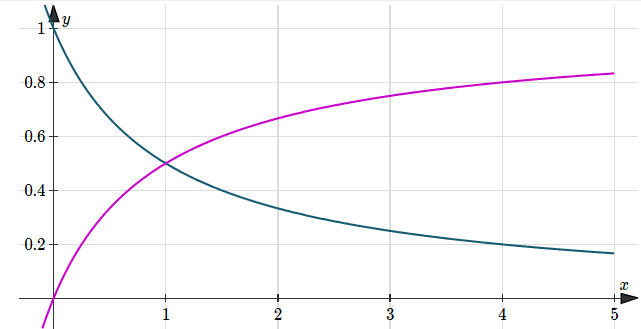
\includegraphics[width=4.3in]
{autoregulons/hill-1.png}
\caption{Plot of $y= 1/(1+x^n)$
and $y=x^n/(1+x^n)$ for $n=1$.}
\label{fig-hill-n-1}
\end{figure}

\begin{figure}[h!]
\centering
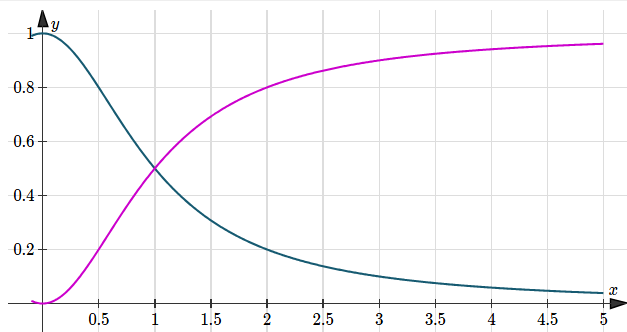
\includegraphics[width=4.3in]
{autoregulons/hill-2.png}
\caption{Plot of $y= 1/(1+x^n)$
and $y=x^n/(1+x^n)$ for $n=2$.}
\label{fig-hill-n-2}
\end{figure}

\begin{figure}[h!]
\centering
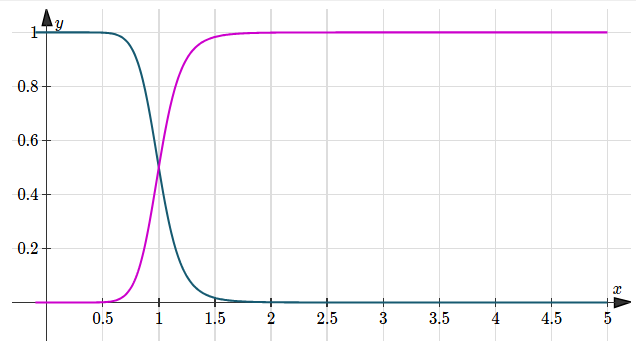
\includegraphics[width=4.3in]
{autoregulons/hill-10.png}
\caption{Plot of $y= 1/(1+x^n)$
and $y=x^n/(1+x^n)$ for $n=10$.}
\label{fig-hill-n-10}
\end{figure}

\section{One Autoregulon}

The ODEs of this chapter can be represented by bnets
in which variables like $x$ and 
their velocities (i.e., time derivatives)
like $\dot{x}$,
are nodes.
Subgraphs of such bnets, especially those
subgraphs that recur frequently as building blocks, are called
a {\bf network motifs}.  The most basic
of the network motifs is the {\bf autoregulon},
which we discuss next.  All bnets
in this chapter can be viewed as {\bf autoregulon
networks}.


This is the autoregulon net motif: 

\beq
\xymatrix{
&\rvx\ar[dd]|{-\alp}\ar[dl]
\\
h(\rvx)\ar[dr]|{1}
\\
&\dot{x}
}\quad
\xymatrix{\\=}
\quad
\xymatrix{
\\
\rvx\ar@{=>}[d]
\\
\dot{\rvx}
}
\xymatrix{\\=}
\quad
\xymatrix{\\\Rect{\rvx}}
\quad
\left\{
\dot{x}=\underbrace{-\alp x + h(x)}_{f(x)}
\right.
\label{eq-1-autoreg}
\eeq
The $-\alp x$ term is called the {\bf removal rate}
and the $h(t)$ term is called the {\bf production rate}.
Eq.(\ref{eq-1-autoreg}) also defines  the 2 symbols
\begin{itemize}
\item double arrow pointing from a random variable and 
to its time derivative,
\item boxed random variable
\end{itemize}
These 2 symbols  will be
used to represent a single autoregulon when we 
represent
networks of autoregulons.


In general, $h(x)$ is either the $\oplus$ or $\ominus$ Hill function.
However, we often use the following approximations
\beq
h(x)=\left\{
\begin{array}{ll}
\beta\indi(x>K)
&(\text{ideal highpass filter})
\\
\beta\indi(x<K)
&(\text{ideal lowpass filter})
\\
h_0+|h_1| x
&(\text{positive feedback})
\\
h_0 -|h_1| x
&(\text{negative feedback})
\end{array}
\right.
\eeq
where $\beta>0$.


\subsection{Autoregulon notation}
Henceforth, we will use

\begin{itemize}
\item
$\xymatrix{\Rect{\rvx}}$ to denote any 
autoregulon $\rvx$

\item
$\xymatrix{\Rect{\rvx^\redoplus}}$ to denote a highpass 
autoregulon $\rvx$

Ref.\cite{alon-book}
denotes this by 
$\xymatrix{\rvx\loopright{3}{}}$

\item
$\xymatrix{\Rect{\rvx^\redominus}}$ to denote a lowpass 
autoregulon $\rvx$

Ref.\cite{alon-book}
denotes this by 
$\xymatrix{\rvx\loopright{3}{@{-|}}}$


\item
$\xymatrix{\Rect{\rvx^\redplus}}$ to denote a positive feedback 
autoregulon $\rvx$


\item  $\xymatrix{\Rect{\rvx^\redminus}}$
to denote a negative feedback 
autoregulon $\rvx$. 



\item $\xymatrix{\rvx\ar[r]^\alp&\rvy}$ to denote $\rvy = \alp \rvx$.

 \item  $\xymatrix{\rvx\ar[r]|\redplus&\rvy}$
to denote
$\xymatrix{\rvx\ar[r]^\alp&\rvy}
$
with $\alp>0$.

\item  $\xymatrix{\rvx\ar[r]|\redminus&\rvy}$
to denote
$\xymatrix{\rvx\ar[r]^\alp&\rvy}$
with $\alp<0$

Ref.\cite{alon-book}
denotes this by $\xymatrix{\rvx\ar@{-|}[r]&\rvy}$


\item  $\xymatrix{\rvx\ar[r]|\redzero&\rvy}$
to denote
$\xymatrix{\rvx\ar[r]^\alp&\rvy}$
with $\alp=0$.

\item  $\xymatrix{\rvx\ar[r]|\redominus^K
&\rvy}$
to denote
$h_\ominus(x)$
for some $K>0$

\item  $\xymatrix{\rvx\ar[r]|\redoplus^K
&\rvy}$
to denote
$h_\oplus(x)$
for some $K>0$

\end{itemize}

Note that 
near $x=K$, $h_{\oplus}$ is
approximately linear
with positive slope.
Hence,  $h_{\oplus}$
is closely related to positive feedback, as their symbols
$\redoplus$ and $\redplus$ suggest. 

The last paragraph is still true if we replace the terms (positive, $\redoplus$, 
$\redplus$) by 
(negative, $\redominus$, 
$\redminus$).

If an arrow in a net has no sign, assume its sign 
might be either plus or minus.

Sometimes we want to write an expression
such as $\alp x -\beta y$ for some $\alp, \beta>0$ but we don't want to specify
the names of the coefficients $\alp, \beta$.
In such cases, we will write $\PP x -\PP y$
instead of $\alp x -\beta y$. In general,
\begin{itemize}
\item
$\PP x$ means $\alp x$ for some $\alp>0$.
\item
$-\PP x$ means $\alp x$ for some $\alp<0$.
\item
$\RR x$ means $\alp x$ for some $\alp\in \RR$.
\end{itemize}


We will be using truth functions
of $x$ 
as well as $t$. For example,
up x-step
$\indi(x>K)$ and 
up t-step $\indi(t>t_1)$.

For any two times $t_1, t_2$ such that $t_1<t_2$, we will 
denote
a {\bf unit t-pulse} by

\beq
\indi_{t_1}^{t_2}(t) = \indi(t_1 < t <t_2)
\eeq
Then we will call a function
$g(x)\indi_{t_1}^{t_2}(t)$,
the pulsed $g(x)$.
For example,
$h_\oplus(x)\indi_{t_1}^{t_2}(t)$
is the pulsed $h_\oplus(x)$.

Note that

\beqa
\indi_{t_1}^{t_2}(t)
&=&\indi(t>t_1)\indi(t<t_2)
\\
&=& \indi(t>t_1)[1-\indi(t>t_2)]
\\
&=&\indi(t>t_1) -\indi(t>t_2)
\eeqa

\subsection{Potential function}

In this section, we will discuss the 
potential function $V(x)$ for autoregulons.
Recall from Chapter \ref{ch-dynamical-sys}
that $f=-\partial_t V$  for a dynamical
system $\dot{x}=f(x)$.

Let

\beq
\dot{x} = \underbrace{-\alp x + h(x)}_{f(x)}
\eeq
and

\beq
h(x)= h_0 + h_1x
\eeq
Then

\beqa
f(x)
&=&h_0
-\underbrace{(\alp-h_1)}_{\alp'} x
\\
&=&
-\alp'(x-x_h)
\eeqa
where
$x_h = \frac{h_0}{\alp'}$.
Hence,



\beq
V-V_0= -\int^x dx\; f(x)=\frac{\alp'}{2}(x-x_h)^2
\label{eq-v-for-general-linear-h}
\eeq
$V_0$ is arbitrary, but note that $V(x)$ must be continuous
because, since $\dot{x}=-\partial_xV(x)$, a jump in $V(x)$
would produce an infinity in $\dot{x}$.

\begin{figure}[h!]
\centering
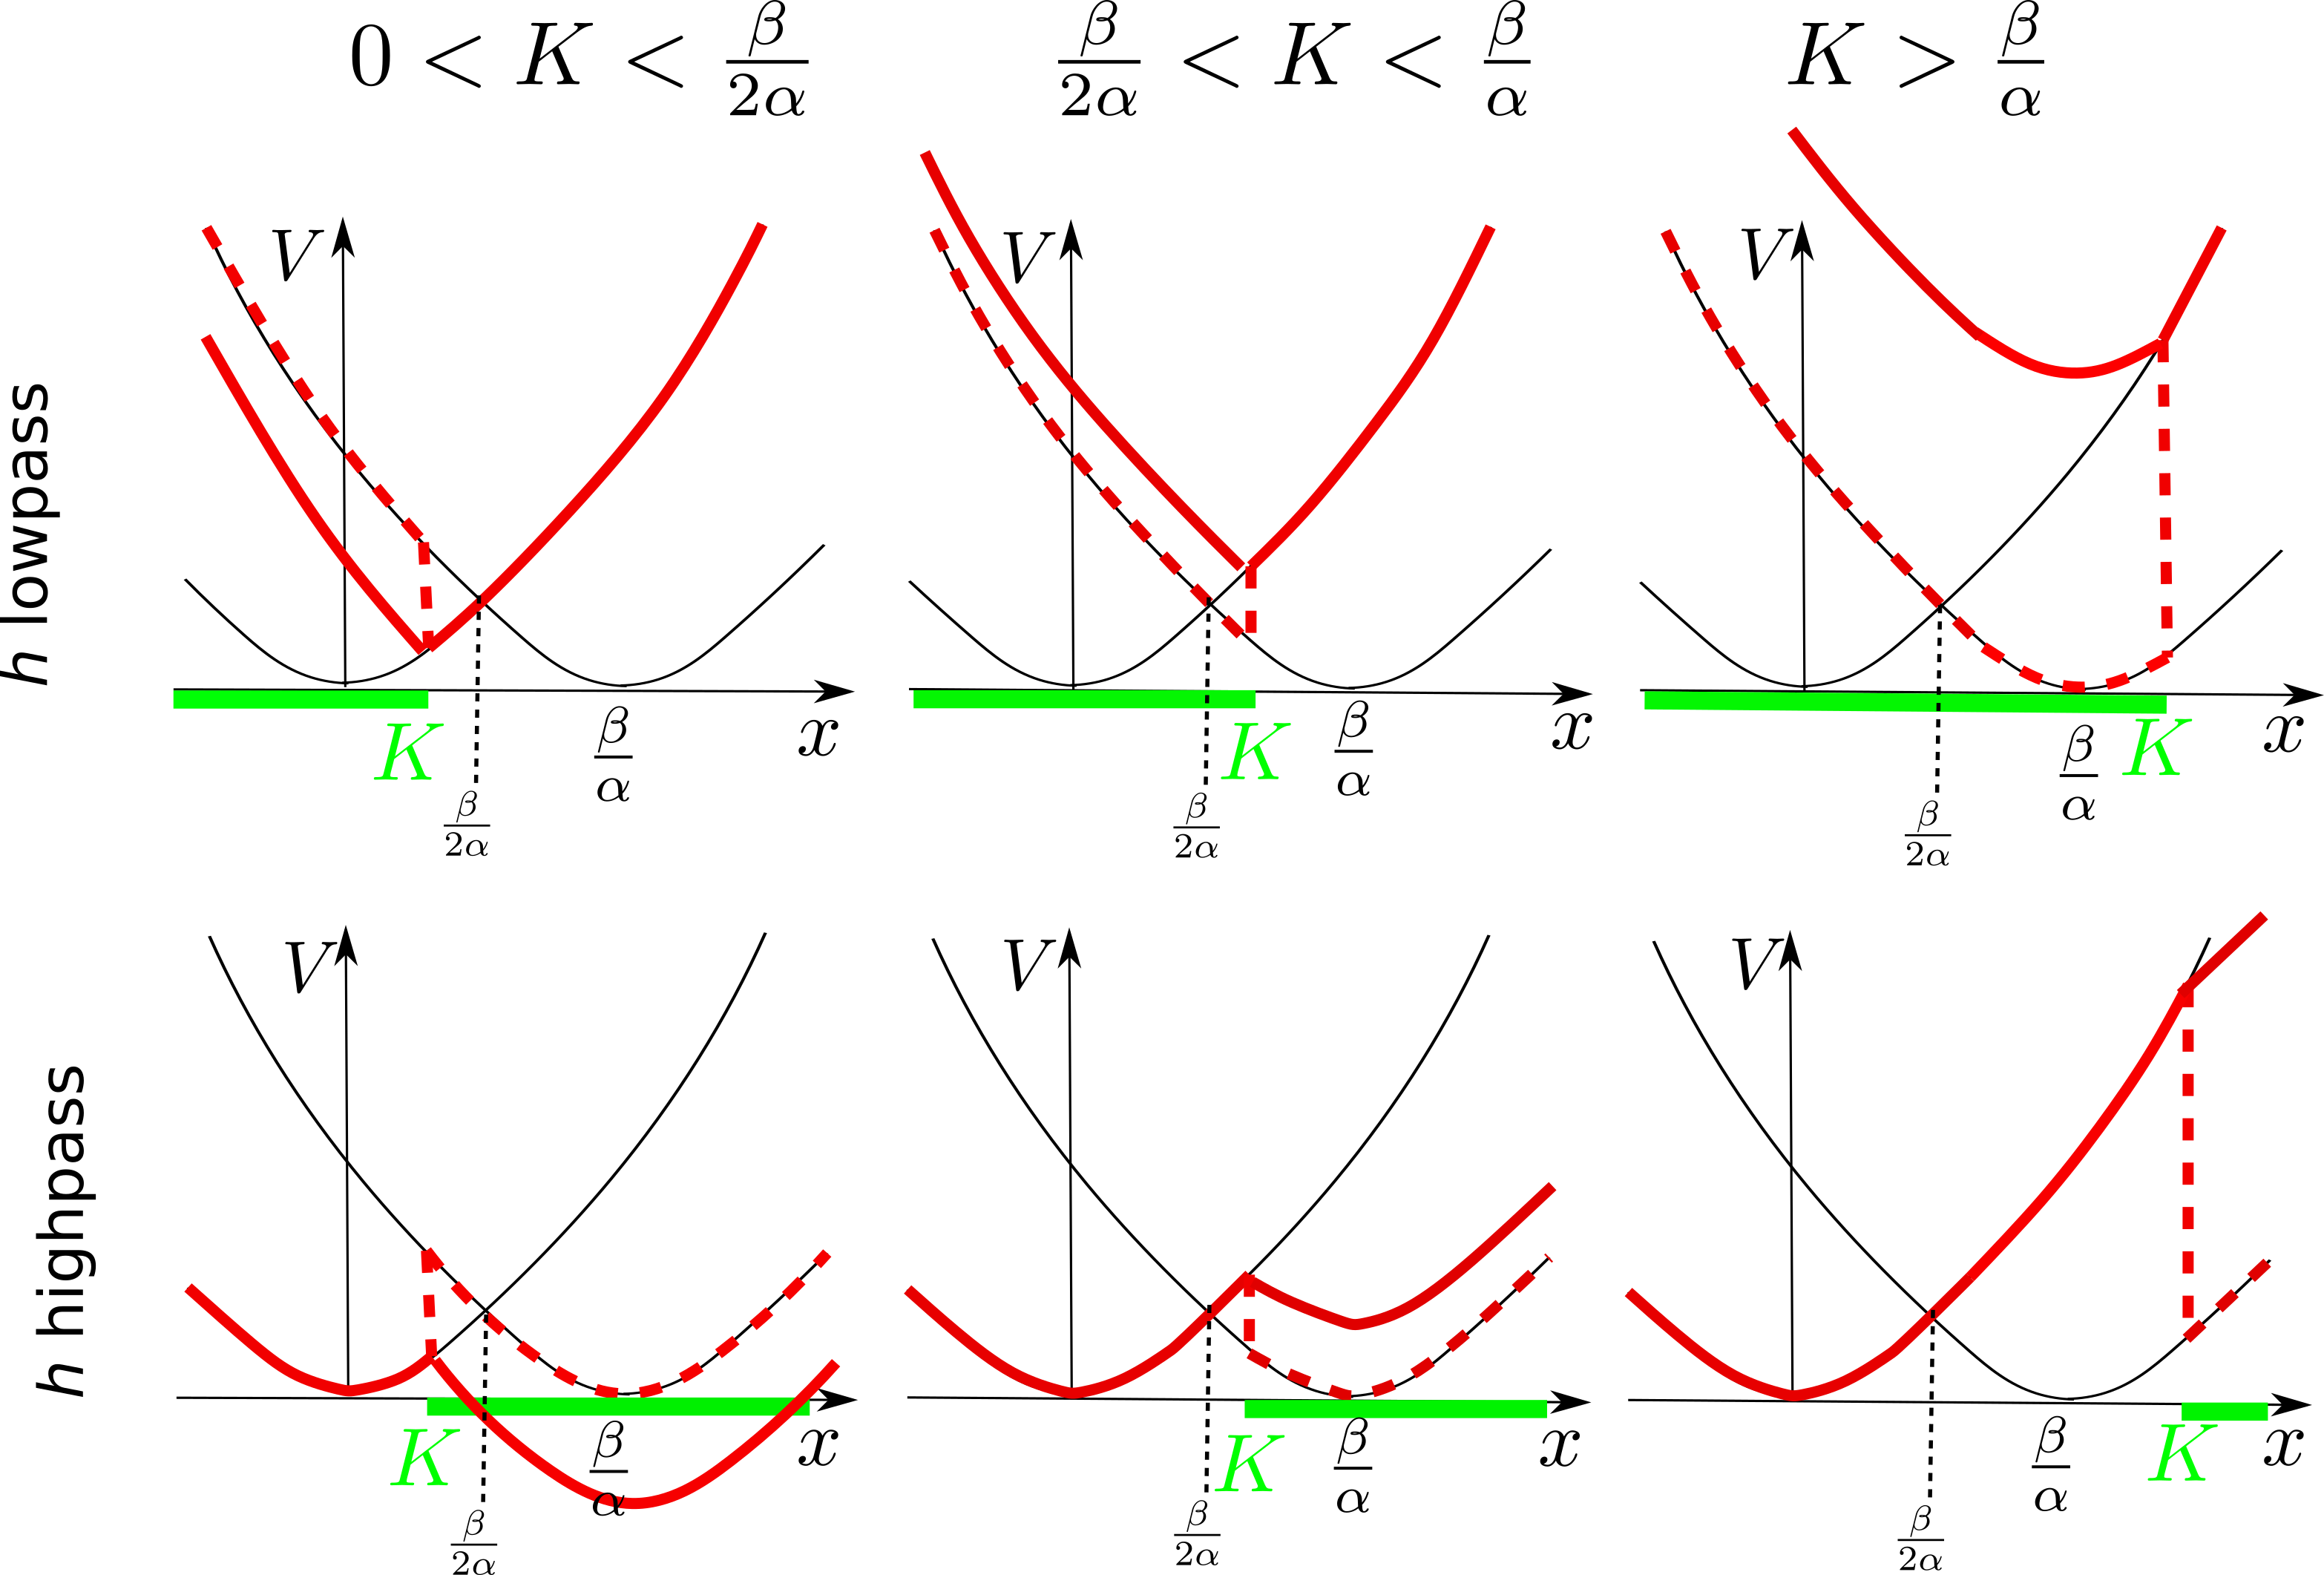
\includegraphics[width=4.7in]
{autoregulons/v-low-high-pass.png}
\caption{ $V(x)$ (in solid, not dashed, red lines),
for an autoregulon with highpass or lowpass $h$,
and for various 
ranges of $K$.
$h(x)$ is zero outside green regions of $x$ axis.
Note that when $V_0=0$, $V$ has two branches: two
parabolas with the same second derivative but different vertices at $x=0$ and $x=\frac{\beta}{\alp}$. 
By symmetry, their intersection is
at $x=\frac{\beta}{2\alp}$,
midway between the vertices.}
\label{fig-v-low-high-pass}
\end{figure}

Eq.(\ref{eq-v-for-general-linear-h})
for linear $h$
can be used to analyze the following
3 cases
in which $h$
is piece-wise linear:

\begin{enumerate}
\item {\bf ideal lowpass filter}

When 

\beq
h(x)=\beta\indi(x<K)
\eeq
we have

\beq
h_0 = \left\{
\begin{array}{ll}
\beta &\text{if $x<K$}
\\
0 & \text{if $x>K$}
\end{array}
\right\}
,\quad
h_1=0
\eeq
Hence,

\beq
V=
\left\{
\begin{array}{ll}
\frac{\alp}{2}(x-x_\beta)^2 + V_0
&\text{if $x<K$}
\\
\frac{\alp}{2}x^2
&\text{if $x>K$}
\end{array}
\right.
\eeq
where 
$x_\beta =\frac{\beta}{\alp}$,
and $V_0$ is defined so that $V(x)$ is the same for $x=K\pm\eps$
where $0<\eps<<0$.

See Fig.\ref{fig-v-low-high-pass} for a plot of this $V$.
From that figure,
we learn that if $h$ is lowpass, the potential has one minimum:

\begin{itemize}[$\checkmark$]
\item at $x=K$ if $K<\frac{\beta}{\alp}$,

\item at $x=\frac{\beta}{\alp}$ if $K>\frac{\beta}{\alp}$.

\end{itemize}

\item {\bf ideal highpass filter}

If 

\beq
h(x)=\beta\indi(x>K)
\eeq
then

\beq
h_0 = \left\{
\begin{array}{ll}
0 &\text{if $x<K$}
\\
\beta & \text{if $x>K$}
\end{array}
\right\},\quad
h_1=0
\eeq
Hence,

\beq
V=
\left\{
\begin{array}{ll}
\frac{\alp}{2}x^2
&\text{if $x<K$}
\\
\frac{\alp}{2}(x-x_\beta)^2 + V_0
&\text{if $x>K$}
\end{array}
\right.
\eeq
where 
$x_\beta =\frac{\beta}{\alp}$,
and $V_0$ is defined so that $V(x)$ is the same for $x=K\pm\eps$
for $0<\eps<<0$.

See Fig.\ref{fig-v-low-high-pass} for a plot of this $V$.
From that figure, we learn that if $h$ is highpass, it has one or two minima:

\begin{itemize}[$\checkmark$]
\item at $x=0$ and $x=\frac{\beta}{\alp}$ if $K<\frac{\beta}{\alp}$,

\item at $x=0$ if $K>\frac{\beta}{\alp}$

\end{itemize}


\item {\bf linear $h$} (positive feedback if $h_1>0$,
negative feedback otherwise)

When

\beq
h(x)\approx h_0 + h_1x
\eeq
we have

\beq
V= \frac{\alp'}{2}(x-x_h)^2
\eeq

See Fig.\ref{fig-v-low-high-pass}
for a plot of this $V$ for various 
choices of $\alp'=\alp-h_1$.

\begin{figure}[h!]
\centering
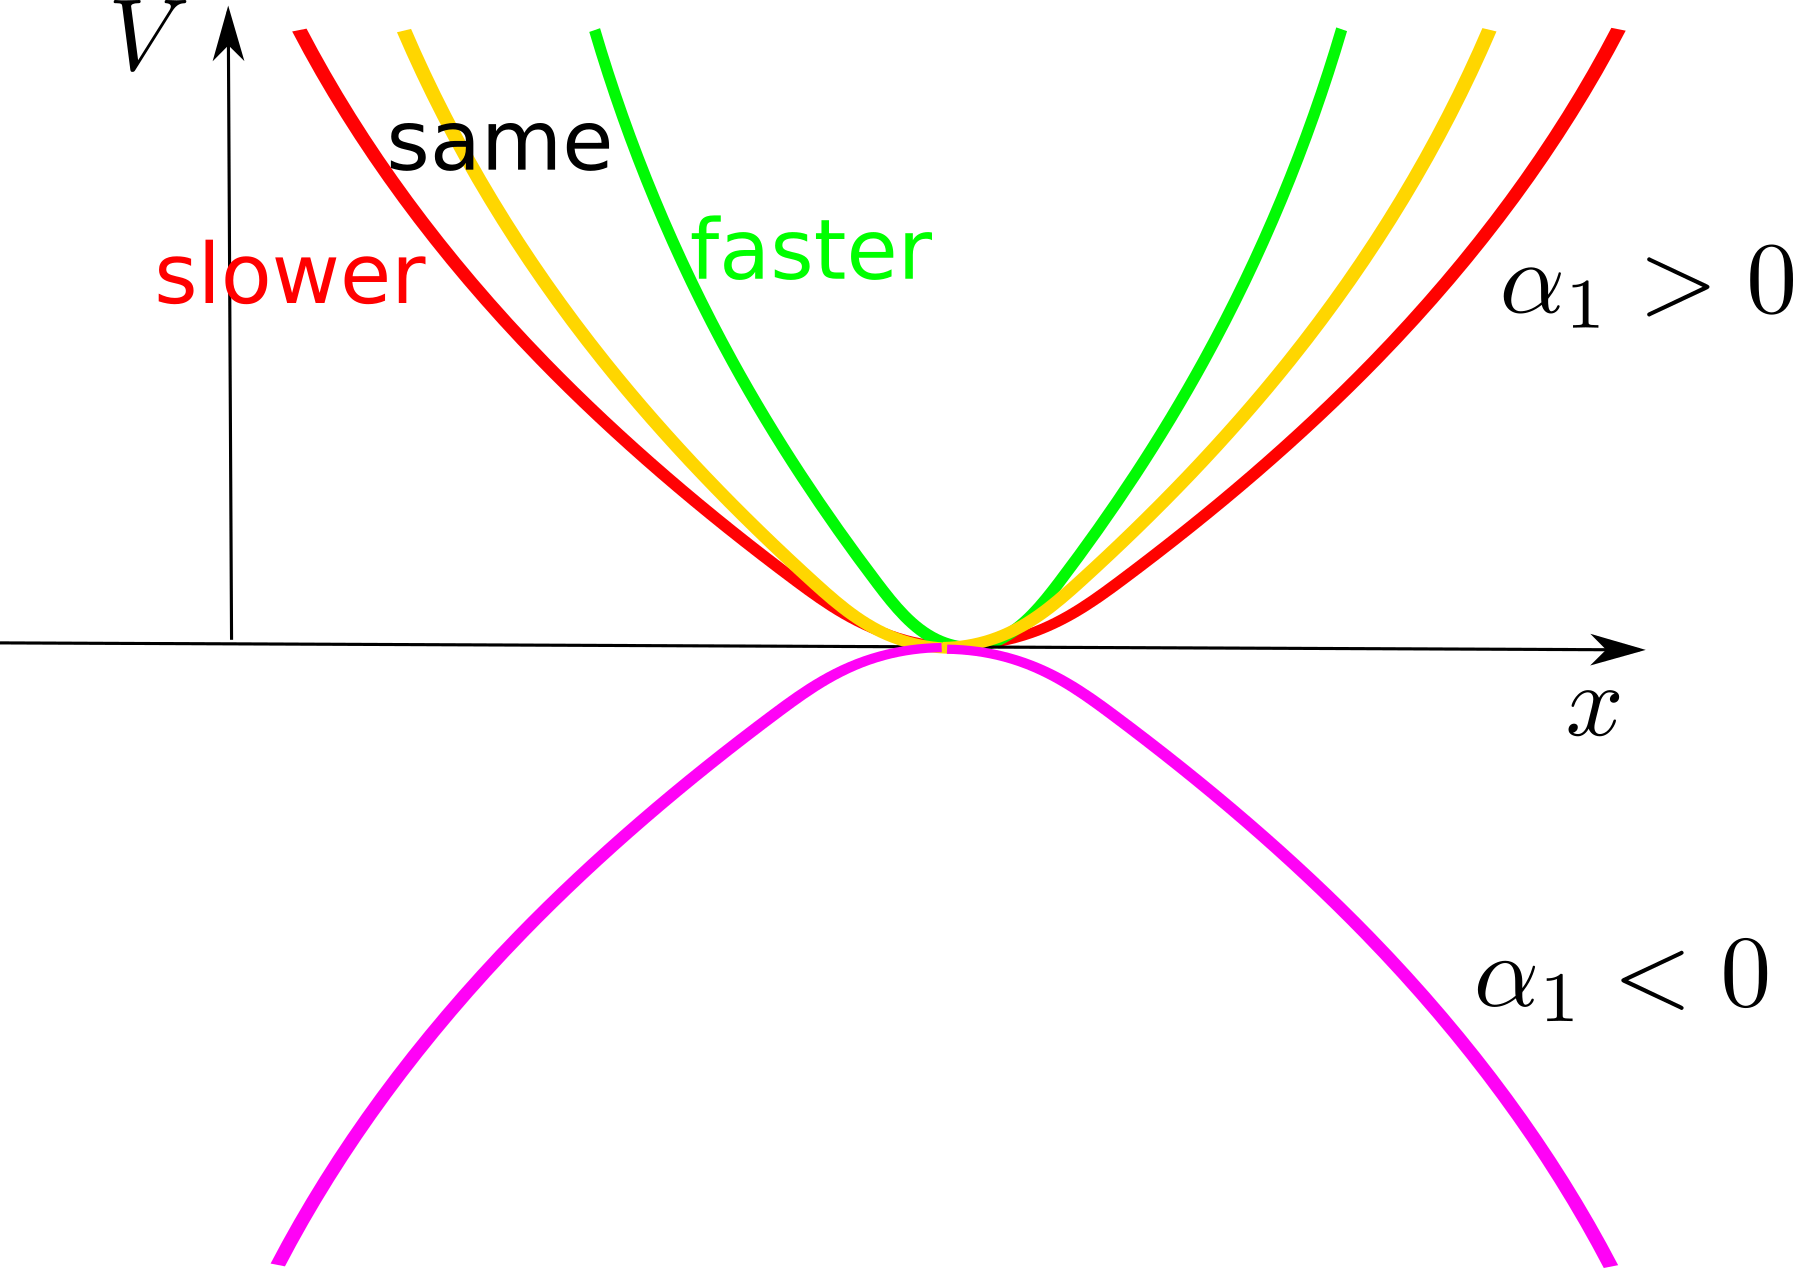
\includegraphics[width=2in]
{autoregulons/v-faster-same-slower.png}
\caption{Plot of $V(x)$ for 
$0<\alp'<\alp$ (slower),
$\alp'=\alp$ (same) and
$\alp'>\alp$ (faster).
Also, plot of $V(x)$ for $\alp'<0$.}
\label{v-faster-same-slower}
\end{figure}
 
\end{enumerate}

\subsection{Linear Expansion of $h$}

In this section, we will
discuss the solution of
the autoregulon ODE
when $h(x)$ is replaced by
its linear approximation.

Let 

\beqa
\dot{x} &=& -\alp x + h_0 + h_1x
\\
&=& -\alp'(x-x_h)
\eeqa
As can be easily checked, the
 most general solution of this ODE is

\beq
x(t)=\underbrace{\xi  e^{-\alp' t} }_{x_h}+
\underbrace{x_h\left[1-e^{-\alp' t}\right]}_{x_p}
\eeq
for some $\xi\in\RR$.
$x_h$ is called the {\bf homogeneous solution} (independent of $h$)\footnote{
$x_h$ satisfies the homogeneous ODE, i.e., the
ODE with $h(x)=0$.
}
and $x_p$ is called the {\bf particular solution} (dependent on $h$).
\footnote{
If we integrate both sides of
$\frac{dx}{-\alp' (x-x_h)}=dt$,
we get the particular solution.
To get the homogeneous 
solution,
we must integrate both sides
of $dx$ = $dt$.}
From this general solution, we conclude that

\begin{itemize}
\item
\ul{if $\alp'<0$, then:} $x(t)$ 
goes exponentially fast  from $\xi $ to $\pm \infty$,
growing as  $(\xi  -x_h)e^{|\alp'|t}$
as $t\rarrow \infty$. 

\item \ul{if $\alp'=0$, then:}
$x(t)$ is constant. 

\item 
\ul{if $\alp'>0$, then:} $x(t)$ goes exponentially fast from
$\xi $ to $x_h$ as $t\rarrow \infty$.
As illustrated in Fig.\ref{fig-fast-normal-slow}, in
this case,
we can have a convergence rate (CR)
 to $x_h$
 that is either faster, the same or slower than $\alp$:
\begin{itemize}[$\checkmark$]

\item \ul{if $0<h_1<\alp$, then:} $\alp'<\alp$, 
CR is slower than $\alp$, {\bf positive autoregulation (PAR)}, positive feedback

\item \ul{if $h_1=0$, then:} $\alp'=\alp$, CR is same as $\alp$,
{\bf zero autoregulation (ZAR)}

\item \ul{if $h_1<0$, then:} $\alp'>\alp$, CR is faster than $\alp$,
{\bf negative autoregulation (NAR)},
negative feedback
\end{itemize}
\end{itemize}


\begin{figure}[h!]
\centering
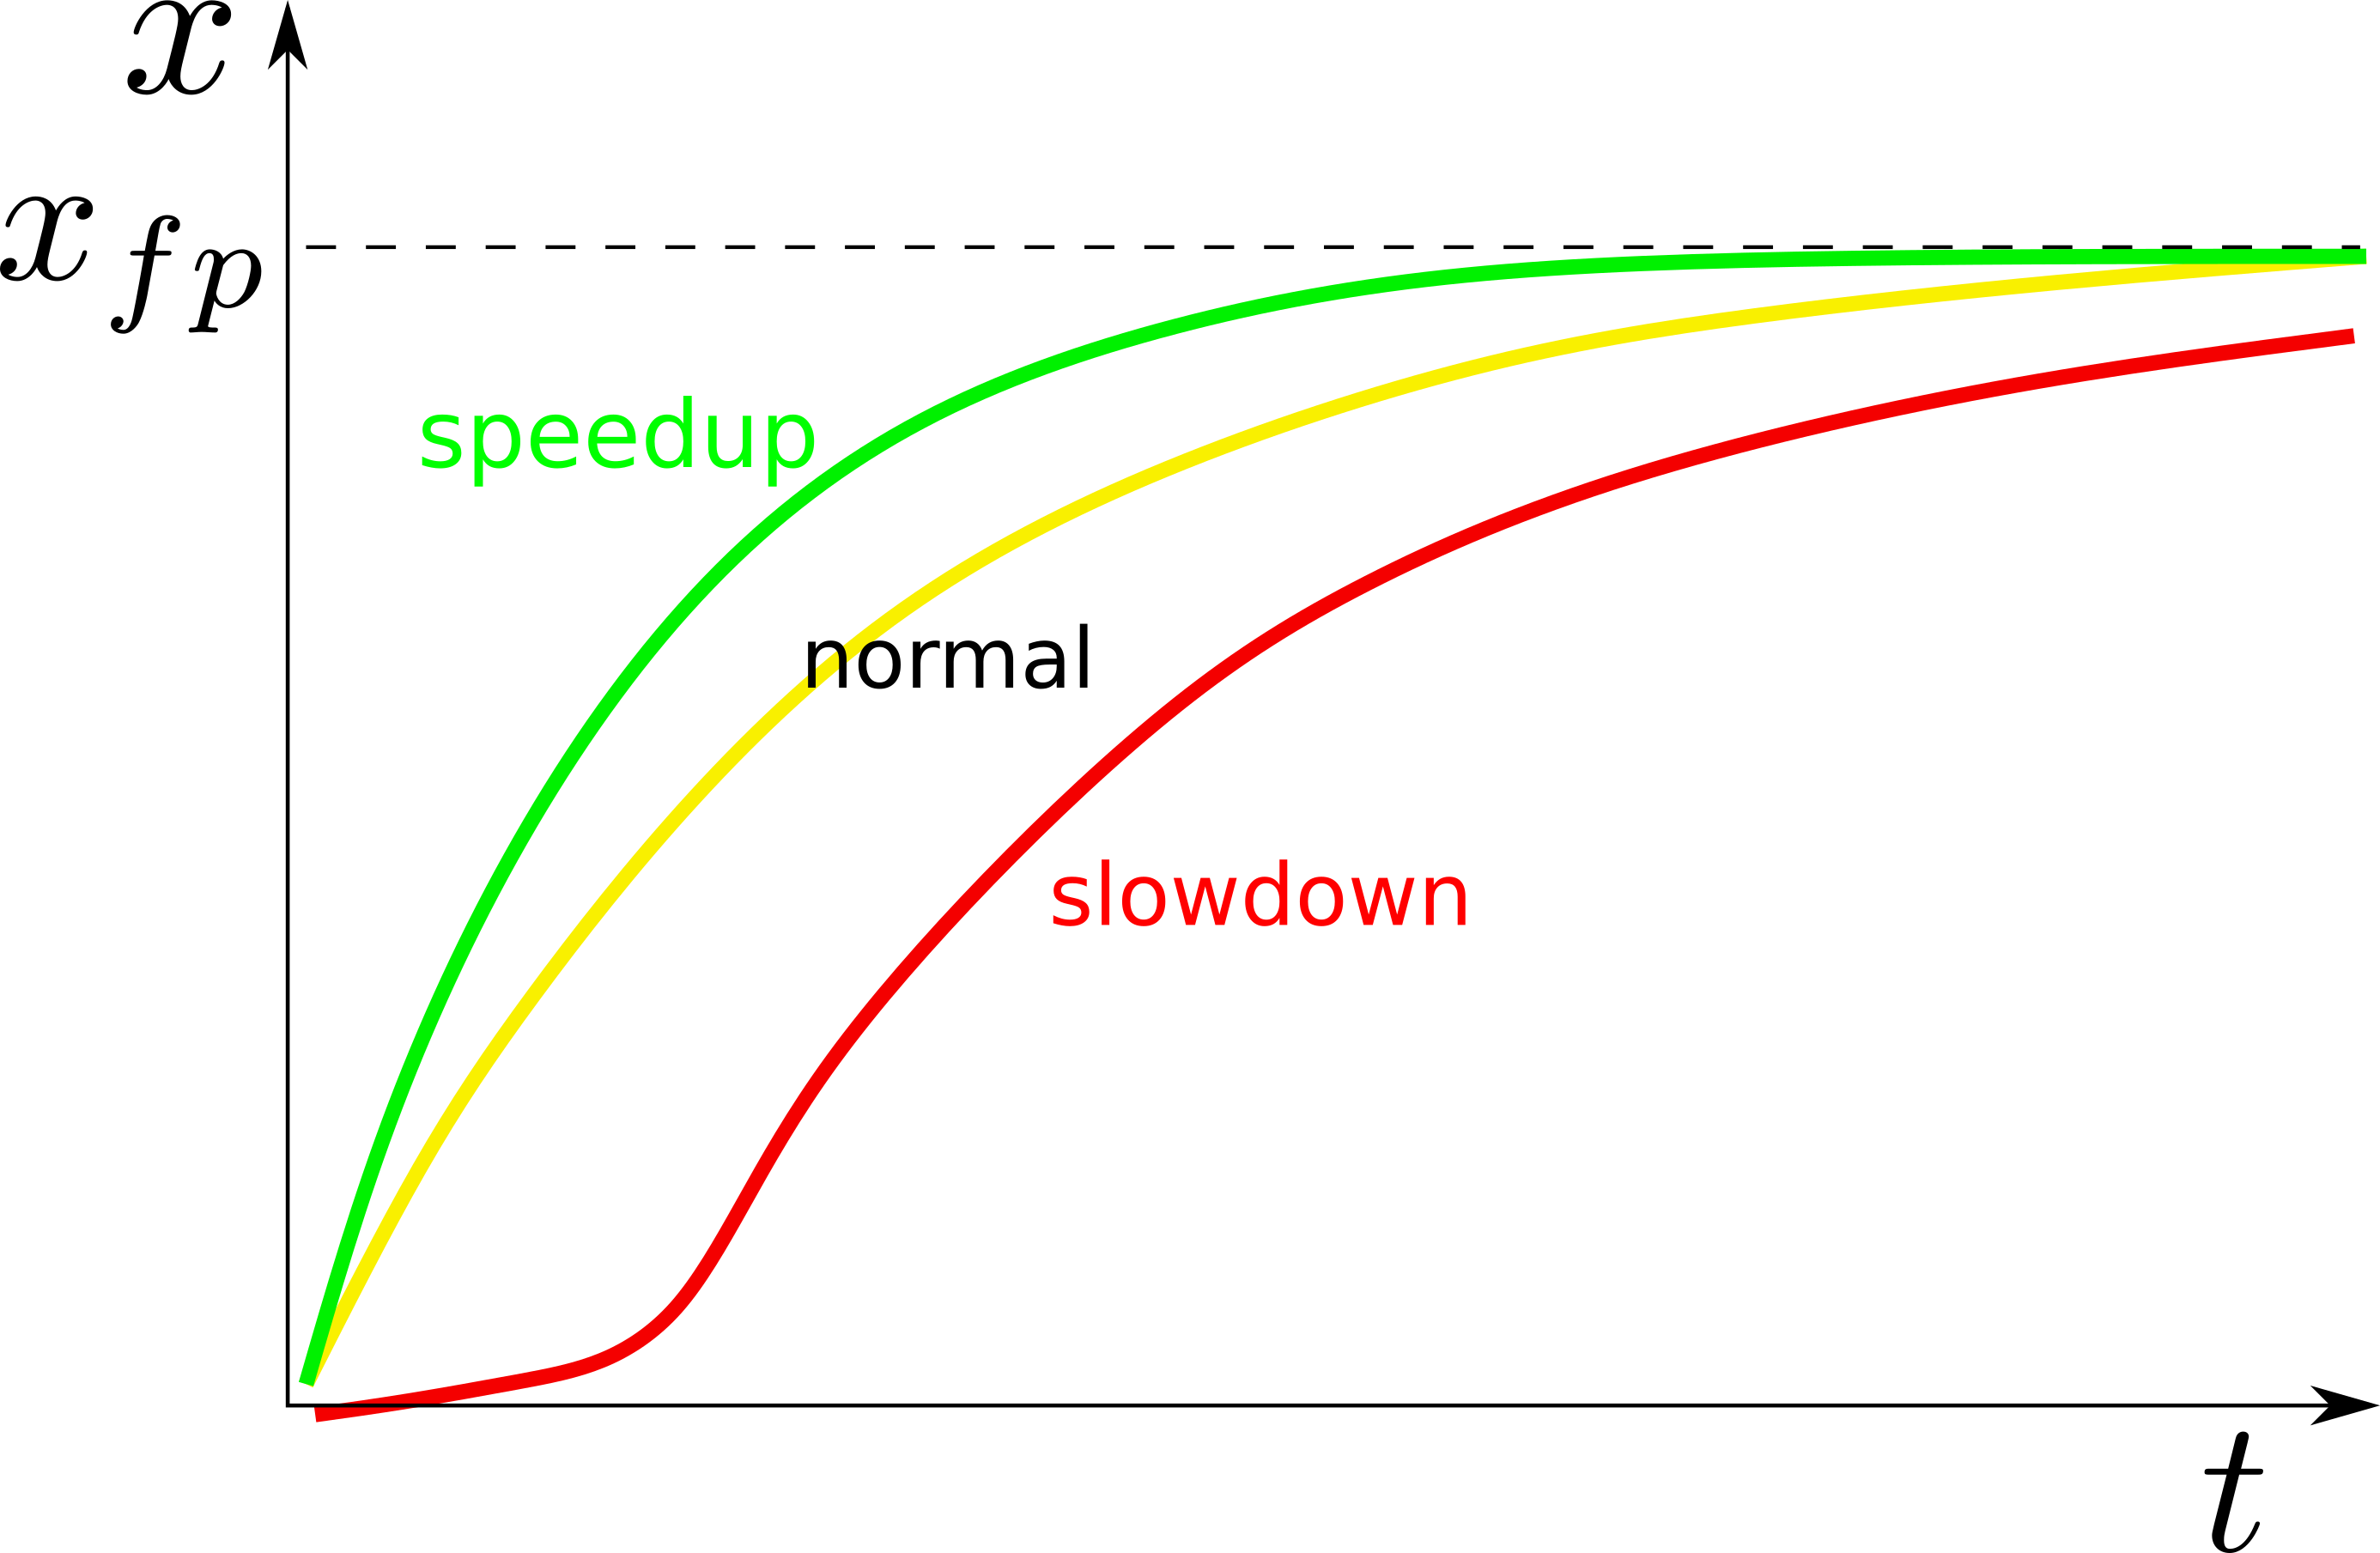
\includegraphics[width=2.5in]
{autoregulons/fast-normal-slow.png}
\caption{For a single autoregulon
with $\alp'>0$, the convergence rate to $x_h$ can 
be either faster, the same or slower than $\alp$.
 }
\label{fig-fast-normal-slow}
\end{figure}




\subsection{Lowpass $h$}
\label{sec-lowpass-h}

\begin{figure}[h!]
\centering
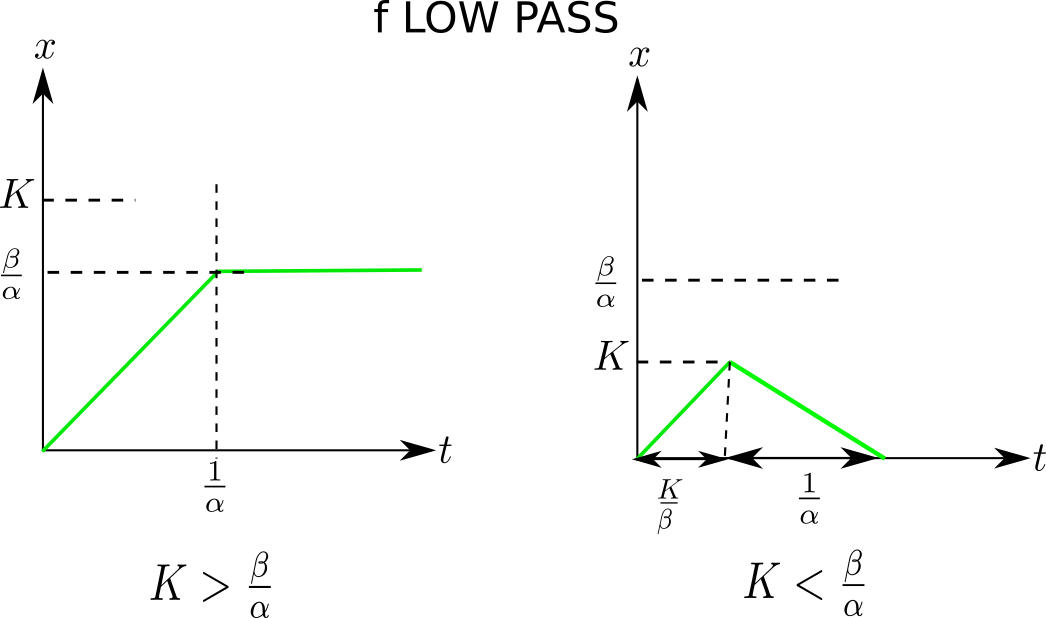
\includegraphics[width=4in]
{autoregulons/autoreg-lowpass.png}
\caption{Approximate $x(t)$
for an autoregulon with a lowpass $h$
and $x(0) =0$}
\label{fig-autoreg-lowpass}
\end{figure}

In this section, we will
discuss the solution of
the autoregulon ODE
when $h(x)$ is
an ideal lowpass filter.
See Fig.\ref{fig-autoreg-lowpass}
for a pictorial
representation of what we will prove.

Let 

\beq
\dot{x} = -\alp x + \beta\indi(x<K)
\eeq
where $\beta, \alp, K>0$. Then

\beq
x= 
\left\{
\begin{array}{ll}
\xi  e^{-\alp t} +
\frac{\beta}{\alp}\left[1-e^{-\alp t}\right]
&\text{ if } x<K
\\
K e^{-\alp (t-t_K)}
&\text{ if } x>K
\end{array}
\right.
\eeq
for some $\xi\in\RR$. To make $x(t)$ continuous at $t=t_K$ when $x=K$,
we must have

\beq
 \xi  e^{-\alp t_K} +
\frac{\beta}{\alp}
\left[1-e^{-\alp t_K}\right]
=
K
\eeq

Note that if $\alp t<<1$, then\footnote{Use $e^x\approx 1 + x$ for $|x|<<1$.}, 

\beqa
x &\approx&
\left\{
\begin{array}{ll}
\xi  + (\beta -\alp \xi )t
&
\text{if }x<K
\\(1-\alp t)
Ke^{\alp t_K}
&
\text{if }x>K
\end{array}
\right.
\eeqa

Assume $x(0)=\xi =0$ for simplicity.
In that case, $x$
increases monotonically towards $\frac{\beta}{\alp}$. 
If $K>\frac{\beta}{\alp}$,
then $x$ reaches $\frac{\beta}{\alp}$
without ever passing through $K$.
So $x(t)$ remains in the $x<K$ branch of the
the solution throughout. 
On the other hand, if $K<\frac{\beta} {\alp}$, 
then,
when $x$ reaches $K$ and tries to
switch branch, it can't do it because
$\partial_x^2V(x)>0$ for $x=K\pm \eps$
so $\dot{x}=0$ at $x=K$.






\subsection{Highpass $h$}
\begin{figure}[h!]
\centering
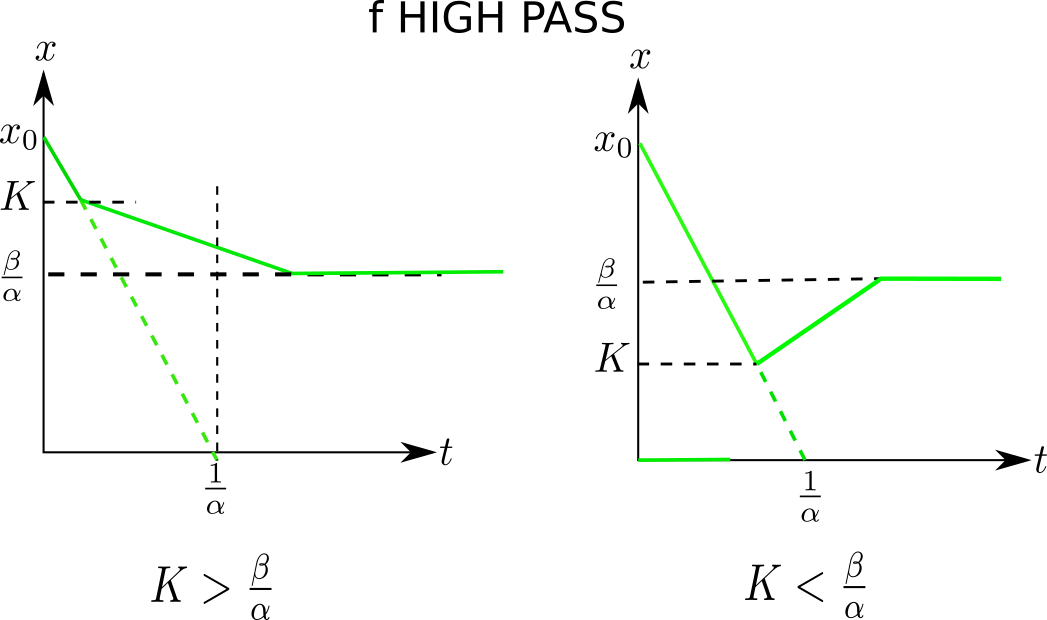
\includegraphics[width=4in]
{autoregulons/autoreg-highpass.png}
\caption{Approximate $x(t)$ for an autoregulon with a highpass $h$
and $x(0)>K$.}
\label{fig-autoreg-highpass}
\end{figure}

In this section, we will
discuss the solution of
the autoregulon ODE
when $h(x)$ is
an ideal highpass filter.
See Fig.\ref{fig-autoreg-highpass}
for a pictorial
representation of what we will prove.

Let 

\beq
\dot{x} = -\alp x + \beta\indi(x>K)
\eeq
where $\beta, \alp, K>0$. Then

\beq
x= 
\left\{
\begin{array}{ll}
K e^{-\alp (t-t_K)} &\text{ if } x<K 
\\
\xi  e^{-\alp t} +
\frac{\beta}{\alp}
\left[ 1-e^{-\alp t}\right]
&\text{ if } x>K
\end{array}
\right.
\eeq
for some $\xi\in\RR$. To make $x(t)$ continuous at $t=t_K$ when $x=K$,
we must have

\beq
K=\xi e^{-\alp t_K}+\frac{\beta}{\alp}
\left[ 1-e^{-\alp t_K}\right]
\label{eq-x0-K-prop}
\eeq

Note that if $\alp t<<1$, then\footnote{Use $e^x\approx 1 + x$ for $|x|<<1$.}, 

\beqa
x &\approx&
\left\{
\begin{array}{ll}
(1-\alp t)
Ke^{\alp t_K}
&
\text{if }x<K
\\
\xi  + (\beta -\alp \xi )t
&
\text{if }x>K
\end{array}
\right.
\eeqa

Unlike when $h$ is a lowpass
filter, 
in this case,
assuming $x(0)=0$ is boring, because $x(t)$
remains at $0$. 
Assume
$x(0) >K$ instead. 

If $K<\frac{\beta}{\alp}$,
$x(t)$ remains always in the $x>K$
branch and plateaus at $x=\frac{\beta}{\alp}$.

If $K> \frac{\beta}{\alp}$,
$x(t)$ switches from the $x>K$ branch to
the $x<K$ branch, and then decays to zero.






\subsection{Pulsed Lowpass $h$}

\begin{figure}[h!]
\centering
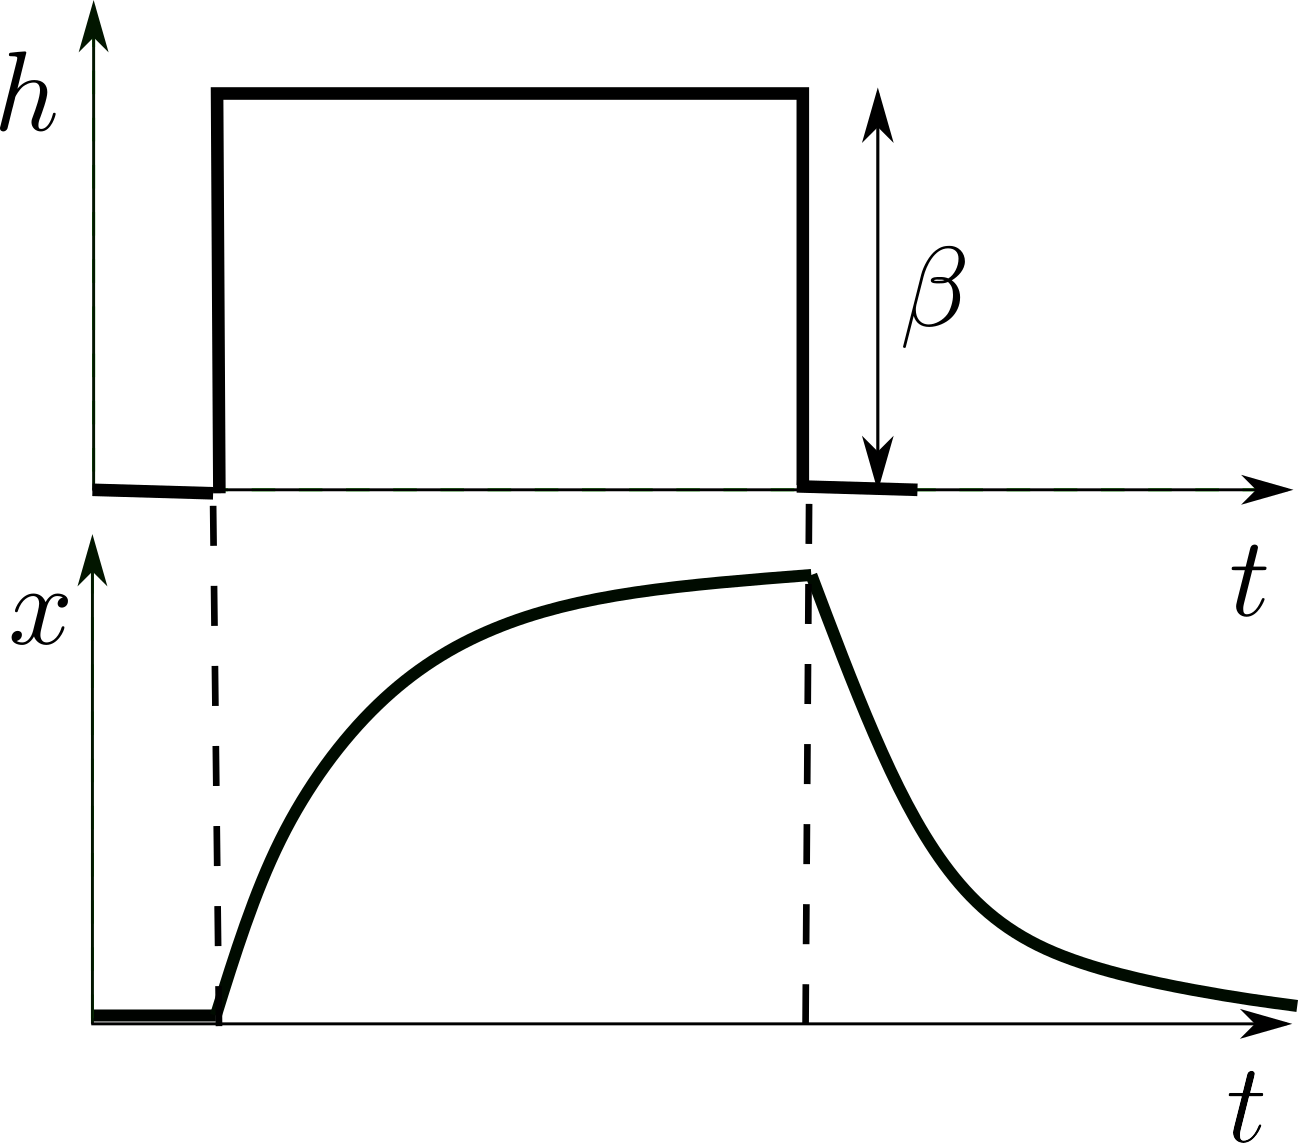
\includegraphics[width=2in]
{autoregulons/pulsed-lowpass.png}
\caption{$h(t)$ and
$x(t)$ for a pulsed lowpass $h$.
}
\label{fig-pulsed-lowpass}
\end{figure}

In this section, we will
discuss the solution of
the autoregulon ODE
when $h(x)$ is
a pulsed ideal lowpass filter.
See Fig.\ref{fig-pulsed-lowpass}
for a pictorial
representation of what we will prove.

Let 

\beq
\dot{x} = -\alp x + \beta\indi(x<K)\indi_{0}^{t_2}(t)
\eeq
where $\beta, \alp, K>0$. 

As discussed in Section \ref{sec-lowpass-h},
if we assume $x(0)=0$,
$x$ reaches $K$ and plateaus there or tends asymptotically
to $x_\infty =\frac{\beta}{\alpha}$.
All this is assumed to happen before $t=t_2$.
Then at $t=t_2$,
the $V$ function becomes a
parabola with $x=0$
as vertex,
so 

\beq
x= x(t_2)e^{-\alp (t-t_2)}
\eeq
 decays exponentially to 0.
 
\subsection{Time dependent production $h(t)$}

Suppose $h$ depends on $t$:
\beq
\dot{x} +\alp x = h(t)
\eeq
As can be easily checked,
the most general solution to this ODE is


\beq
x=
x(0)e^{-\alp t}
+e^{-\alp t}
\int^t_0 dt\;
e^{\alp t}h(t)
\label{eq-h-t-gen-sol}
\eeq

If both $h$ and $\alp$ depend on $t$,
as in

\beq
\dot{x} +\alp(t) x = h(t)
\eeq
then the solution is still 
given by Eq.(\ref{eq-h-t-gen-sol})
if we replace
 

\beq
\alp t\rarrow \int_0^t dt'\; \alp(t')
\eeq



\subsection{Fixed Points}

The fixed points of an autoregulon satisfy

\beq
0=\dot{x}=-\alp x + h(x)
\eeq
Thus, they occur whenever the removal and production curves
$y=\alp x$ and $y=h(x)$ intersect. When $h(x)$ is 

\begin{itemize}
\item
a straight line as in positive or negative
feedback
\item an $\ominus$ Hill function or 
its large $n $ limit, an ideal lowpass filter
\end{itemize}
then
there is just one intersection. But when
$h(x)$ is 

\begin{itemize}
\item an $\oplus$ Hill function or 
its large $n $ limit, an ideal highpass filter
\end{itemize}
then
$y=\alp x$ and $y=h(x)$ can intersect at 1, 2 or 3 points.
Fig.\ref{fig-source-sink-source} shows 
the case where there are 3 intersections, leading to 3 fixed points,
one source and two sinks.

\begin{figure}[h!]
\centering
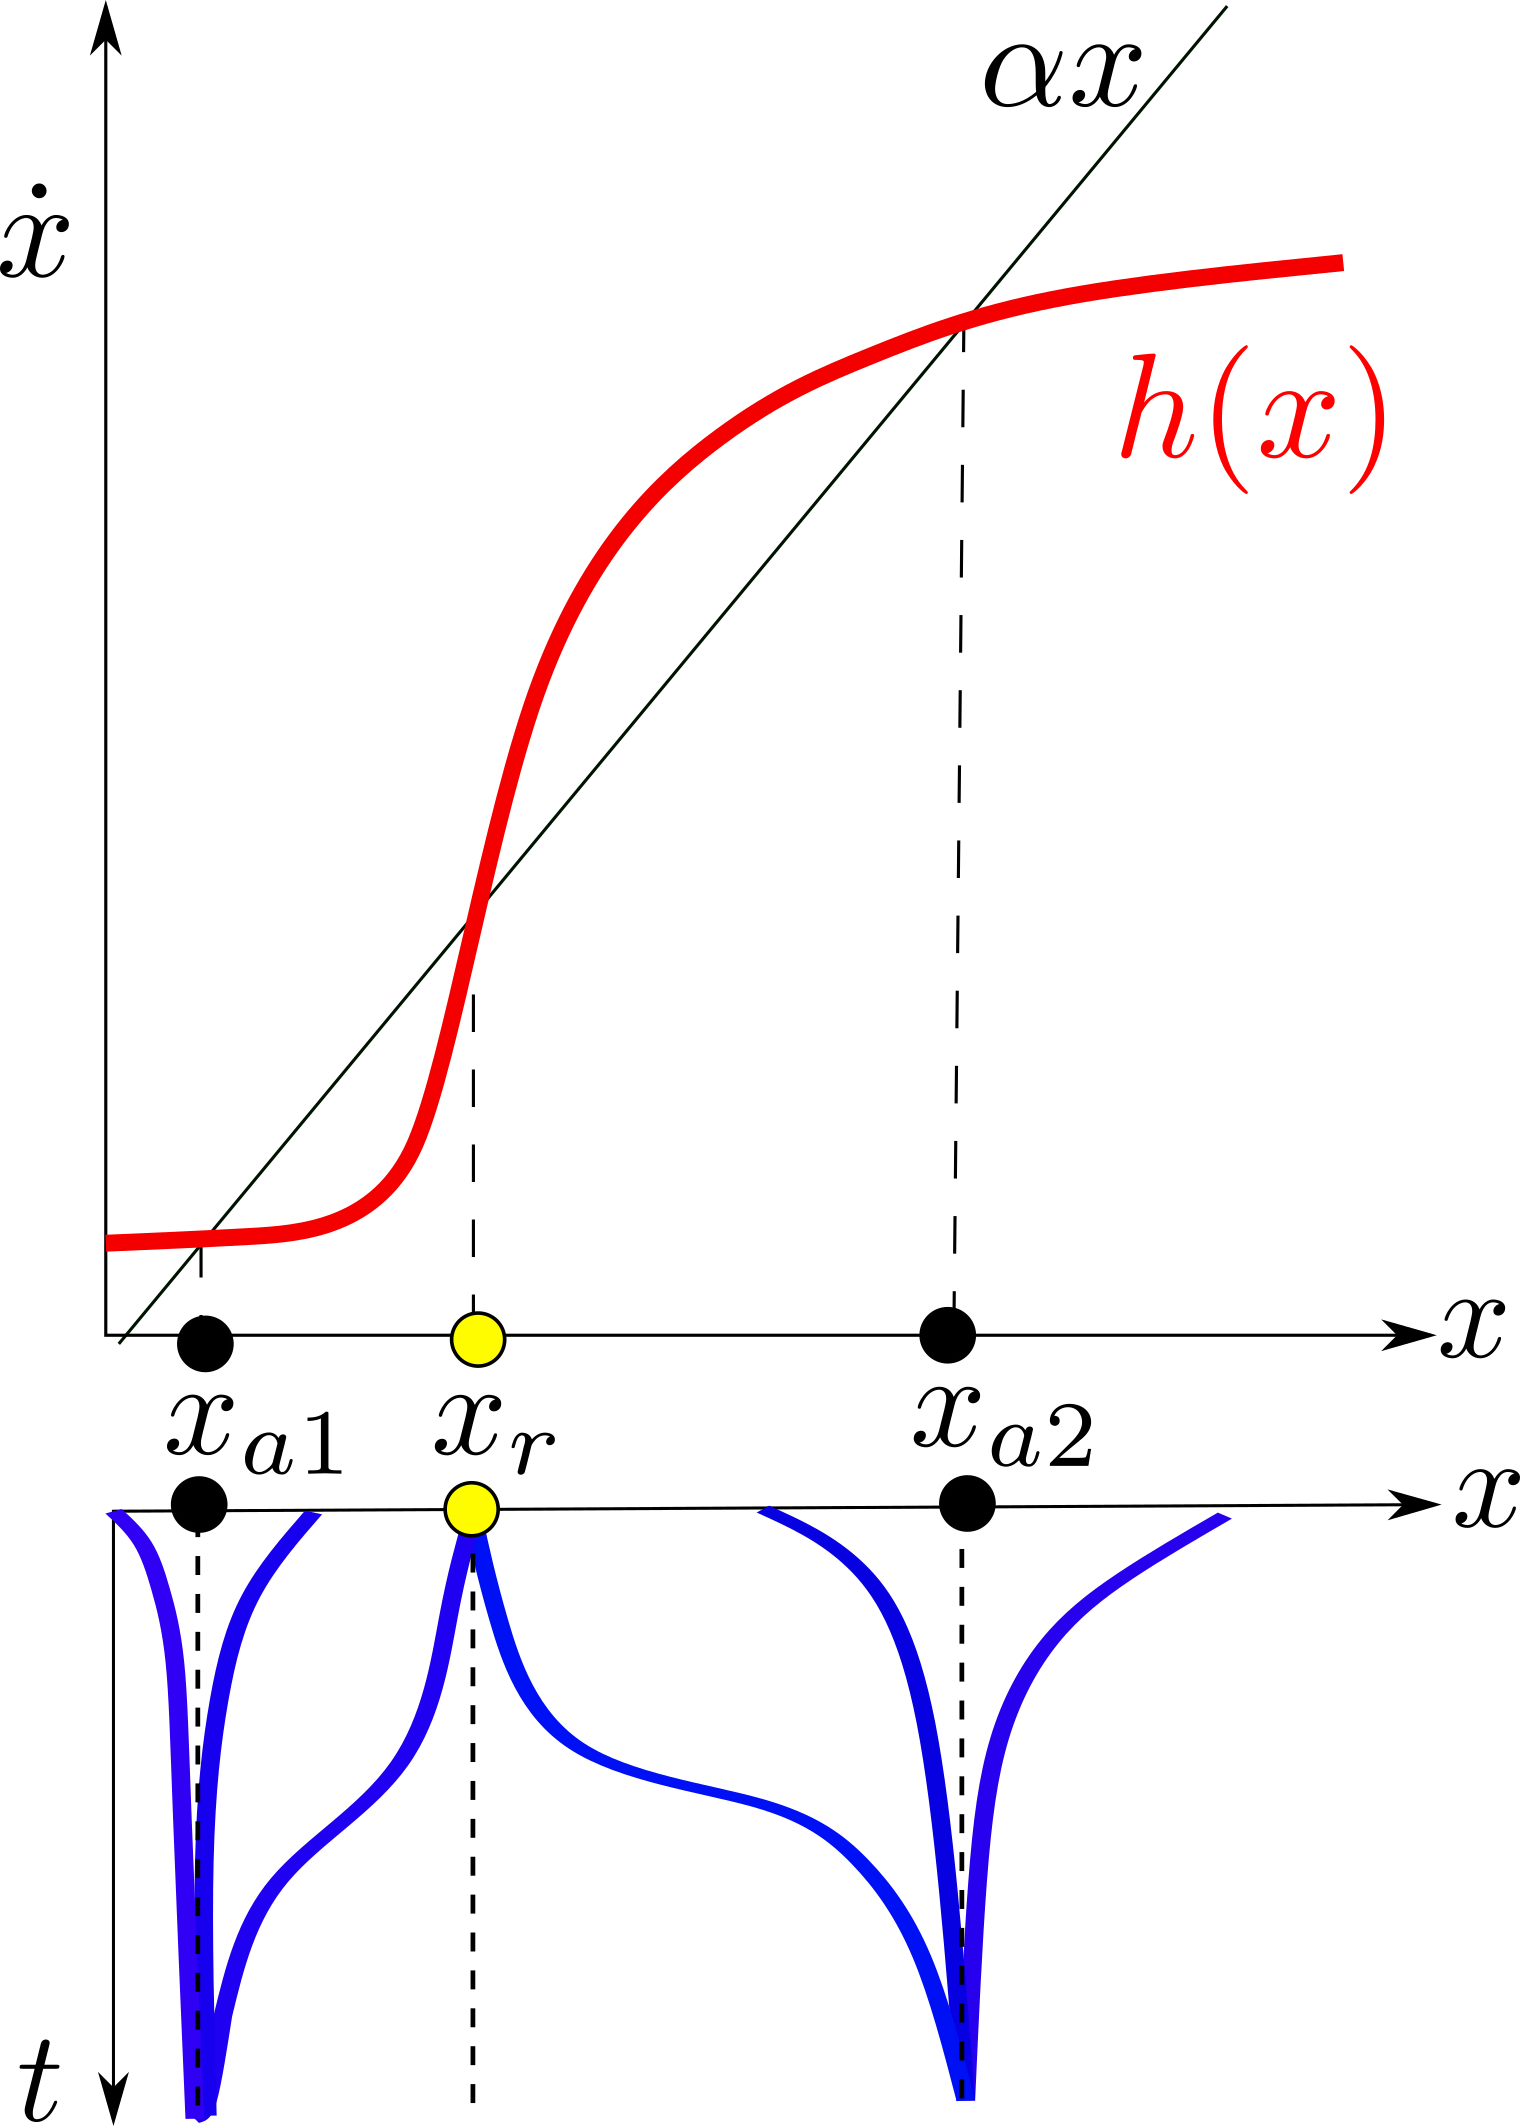
\includegraphics[width=2in]
{autoregulons/source-sink-source.png}
\caption{For single autoregulon $\dot{x}(t)=-\alp x + h(x)$, 
the fixed points occur at the intersection of the
curves $y=\alp x$ and $y=h(x)$. In this case,
there are 3 intersections, leading to 3 fixed points. This can be used as a switch, with $x_A$=OFF=LOW, $x_B$=ON=HIGH. (bistability)
}
\label{fig-source-sink-source}
\end{figure}


\begin{figure}[h!]
\centering
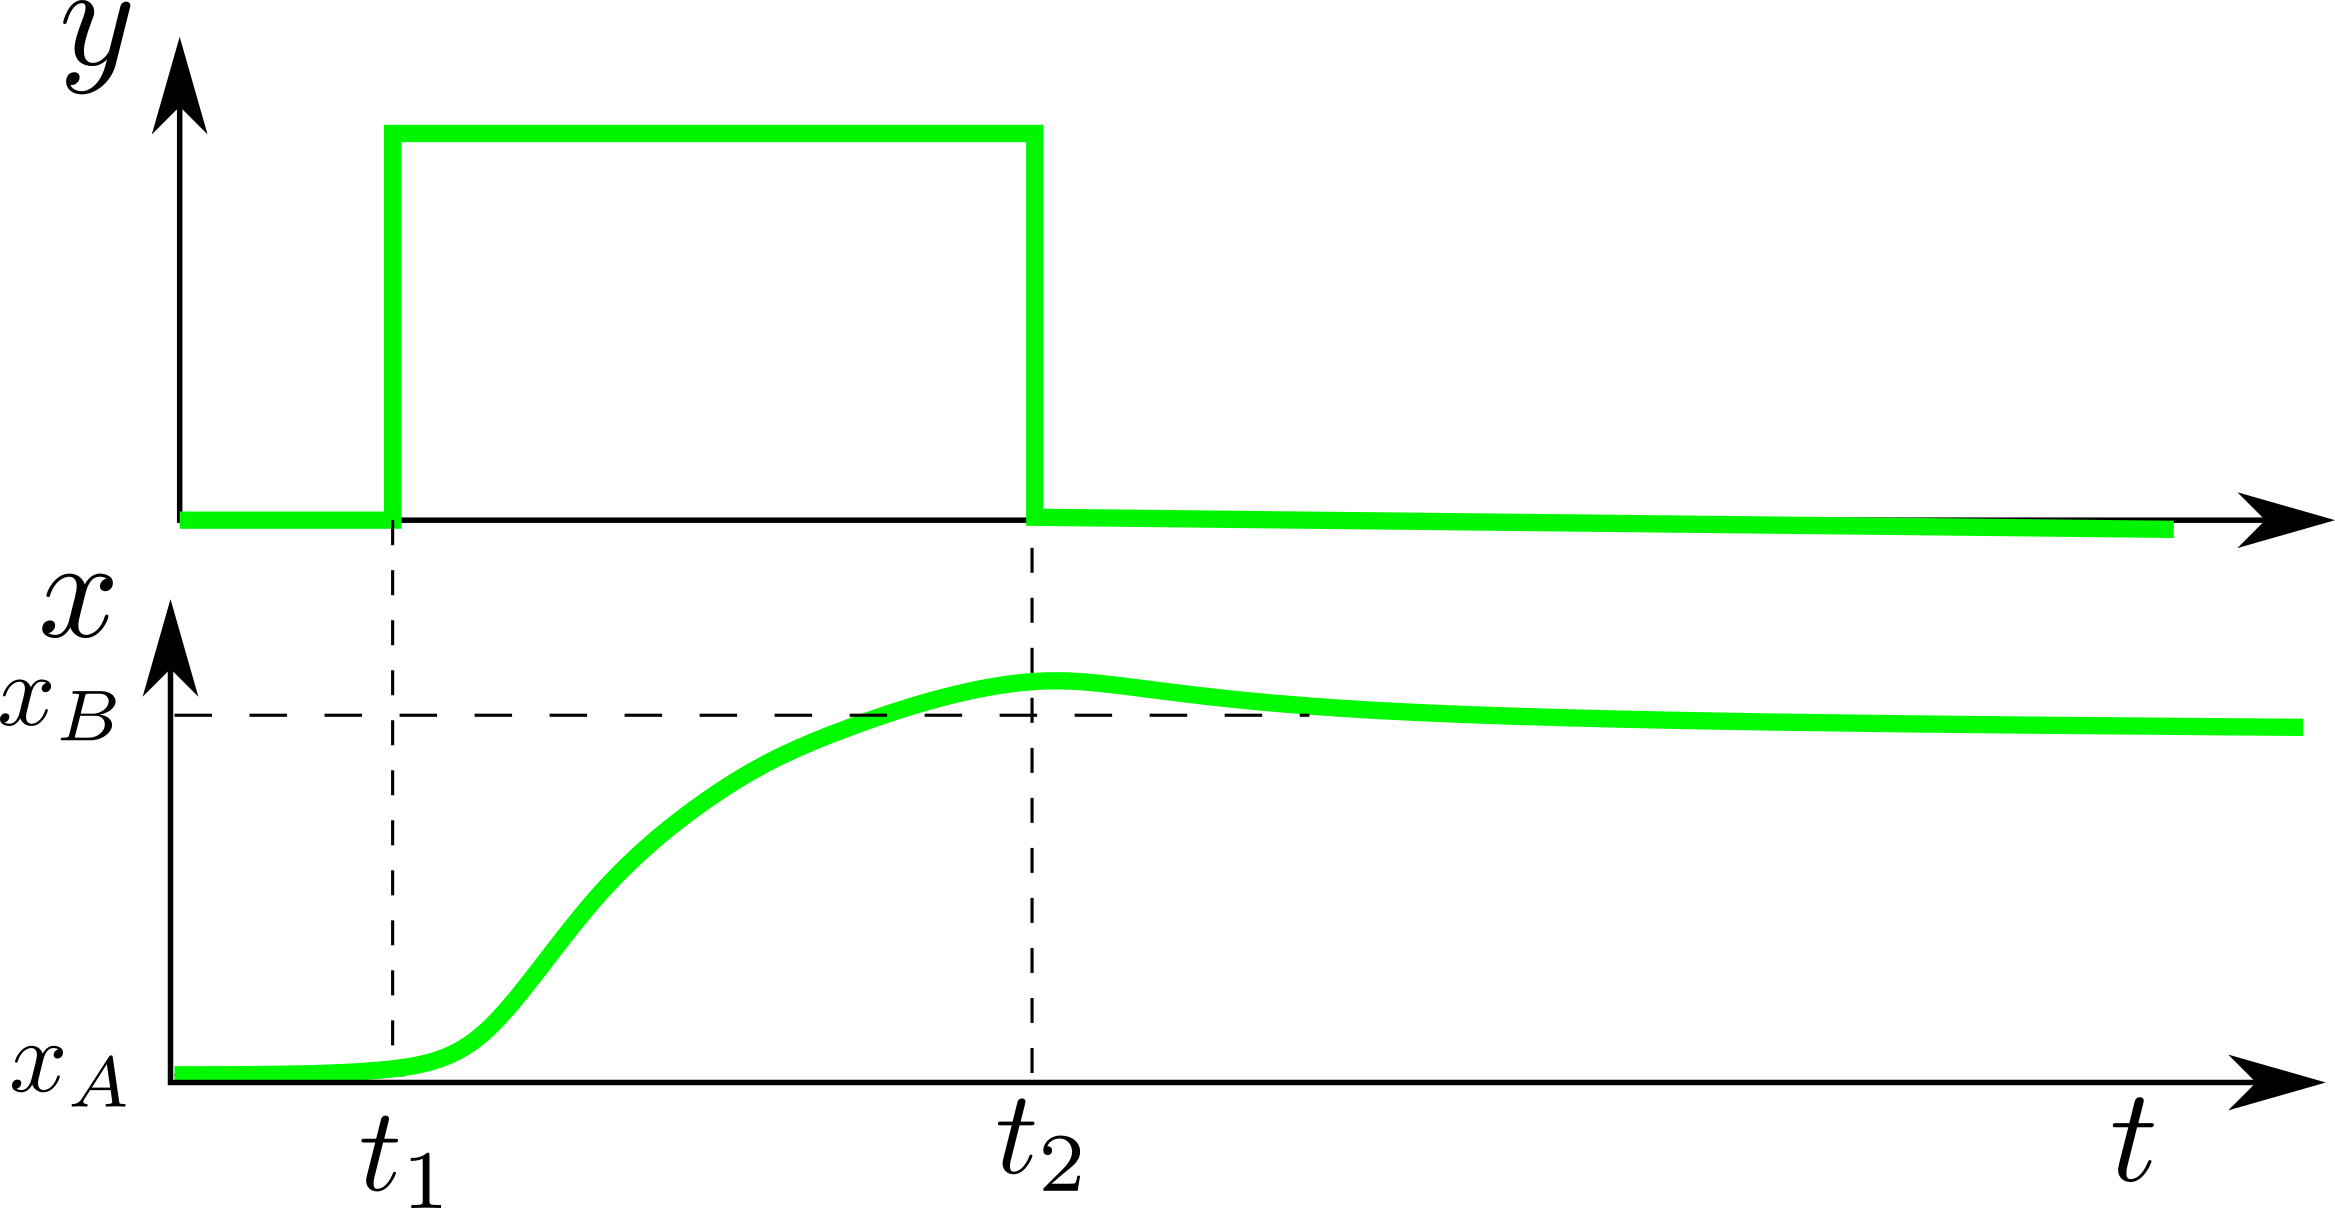
\includegraphics[width=3.5in]
{autoregulons/x-y-memory.png}
\caption{$x$ switched from 
sink $A$ to sink $B$
by a pulse in $y$.}
\label{fig-x-y-memory}
\end{figure}

Fig.\ref{fig-x-y-memory}
shows how an autoregulon
$\rvx$ can 
provide {\bf long term memory}.
The process is described by the ODE

\beq
\dot{x}= -\alp x + h_\oplus(x) + \gamma\indi_{0}^{t_2}(y)
\eeq
Assuming the system is initially in sink $A$,
the $y$ pulse jolts the system to sink $B$.


\section{Two autoregulons}

In this section, we consider bnets
consisting of 2 autoregulons
connected to each other; i.e.,
we will consider
special cases of bnets such as

\beq
\begin{array}{c}
\xymatrix@C=6pc@R=1pc{
\rvx \ar@{=>}[dd]\ar[ddr]|<<<<{}
& \rvy \ar@{=>}[dd]\ar[ddl]|<<<<{}
\\
&
\\
\dot{\rvx}
&\dot{\rvy}
}
\xymatrix{\\
\quad=\quad}
\xymatrix@C=5pc{
\\
\Rect{\rvx}
\fbackar{r}
{}
{}
&
\Rect{\rvy}}
\\
\left\{
\begin{array}{l}
\dot{x}= f_1(x) + \RR y
\\
\dot{y} = f_2(x) + \RR x
\end{array}
\right.
\end{array}
\eeq
and

\beq
\begin{array}{c}
\xymatrix@C=4pc@R=1pc{
\rvx \ar@{=>}[dd]\ar[ddrr]|<<<<{}
\ar[r]
&\bigotimes\ar[ddl]\ar[ddr]
& \rvy \ar@{=>}[dd]\ar[ddll]|<<<<{}
\ar[l]
\\
&
\\
\dot{\rvx}
&
&\dot{\rvy}
}\quad
\xymatrix{\\
\quad=\quad}
\xymatrix@R=4pc@C=3pc{
\Rect{\rvx}\widefbackar{rr}{}{}
\fbackar{r}{}{}
&\bigotimes\fbackar{r}{}{}
&\Rect{\rvy}
}
\\
\left\{
\begin{array}{l}
\dot{x}= f_1(x) + \RR y +\RR xy
\\
\dot{y}= f_2(y) + \RR x + \RR xy
\end{array}
\right.
\end{array}
\eeq
The   \qt{population product}  term $xy$
is typical of predator-prey models (see Section \ref{sec-predator-prey}).

\subsection{Linearized $(+)(-)$}

In this section, we consider the
following bnet, which we call
the {\bf linearized $(+)(-)$}:

\beq
\xymatrix@C=5pc
{\Rect{\rvx}
\fbackar{r}{\redminus}{\redplus}
&\Rect{\rvy}
}
\quad
\left\{
\begin{array}{l}
\dot{x}=-\alp_1 x + \gamma_1 y
\\
\dot{y}= -\alp_2y - \gamma_2 x
\end{array}
\right.
\eeq

If $\vec{x}=(x, y)^T$ and $\dot{\vec{x}}=A \vec{x}$, then

\beq
A = \left[
\begin{array}{cc}
-\alp_1 & \gamma_1
\\
-\gamma_2& -\alp_2 
\end{array}
\right]
\eeq
so

\beq
\begin{array}{l}
\delta = \det A = \alp_1 \alp_2+
\gamma_1 \gamma_2 >0
\\
\tau =\tr A =-(\alp_1 +\alp_2) <0
\end{array}
\eeq
and

\beqa
\Delta &=&\tau^2-4\delta 
\\
&=&
(\alp_1 +\alp_2)^2 - 4\alp_1\alp_2 -4\gamma_1\gamma_2
\\
&=&
(\alp_1-\alp_2)^2 -4\gamma_1\gamma_2
\eeqa

See Chapter \ref{ch-dynamical-sys}
and in particular Fig.\ref{fig-wiki-pp} for what this entails. This system has a sink at $(x,y)=(0,0)$
(because $\tau<0$)
and may or may not oscillate (depending
on the sign of $\Delta$).


\subsection{Linearized $(-)^2$ or $(+)^2$}


In this section we consider the following bnets,
which we call 
the {\bf linearized double positive and double negative (or
$(-)^2$ and $(+)^2$, for short) feedback loops}

\beq
\begin{array}{ccc}
(a)
&\xymatrix@C=5pc
{\Rect{\rvx}
\fbackar{r}{\redminus}
{\redminus}
&\Rect{\rvy}
}
&
\left\{
\begin{array}{l}
\dot{x}=-\alp_1 x - \gamma_1 y
\\
\dot{y}= -\alp_2y - \gamma_2 x
\end{array}
\right.
\\
\\
(b)&
\xymatrix@C=5pc
{\Rect{\rvx}
\fbackar{r}{\redplus}
{\redplus}
&\Rect{\rvy}
}
&
\left\{
\begin{array}{l}
\dot{x}=-\alp_1 x + \gamma_1 y
\\
\dot{y}= -\alp_2y + \gamma_2 x
\end{array}
\right.
\end{array}
\eeq


If $\vec{x}=(x,y)^T$ and $\dot{\vec{x}}=A x$,
then 
\begin{itemize}
\item for $(a)$
\beq
A = \left[
\begin{array}{cc}
-\alp_1 & -\gamma_1
\\
-\gamma_2 & -\alp_2
\end{array}
\right]
\eeq
so

\beq
\begin{array}{l}
\tau =\tr A =-(\alp_1 +\alp_2) <0
\\
\delta = \det A = \alp_1 \alp_2
-\gamma_1 \gamma_2
\end{array}
\eeq

\item for $(b)$:
\beq
A = \left[
\begin{array}{cc}
-\alp_1 & \gamma_1
\\
\gamma_2 & -\alp_2
\end{array}
\right]
\eeq
so

\beq
\begin{array}{l}
\tau =\tr A =-(\alp_1 +\alp_2) <0
\\
\delta = \det A = \alp_1 \alp_2
-\gamma_1 \gamma_2
\end{array}
\eeq

\end{itemize}

Since both $(a)$ and $(b)$ have the same
$(\tau, \delta)$,
they have the same discriminant $\Delta$,
given by

\beqa
\Delta &=&\tau^2-4\delta 
\\
&=&
(\alp_1 +\alp_2)^2 - 4\alp_1\alp_2 +4\gamma_1\gamma_2
\\
&=&
(\alp_1-\alp_2)^2+ 4\gamma_1\gamma_2>0
\eeqa

See Chapter \ref{ch-dynamical-sys}
and in particular Fig.\ref{fig-wiki-pp} for what that entails. This system has a sink at $(x,y)=(0,0)$ (because $\tau<0$) and does not oscillate (because $\Delta>0$).

\subsection{Genetic Toggle Switch}

In the linear approximation (or the case of $n=1$ Hill functions), the two autoregulon system has only 1 sink. In this section, we consider the nonlinear case with two sinks and one source. The two sinks can be used as
ON, OFF states of a switch.

In this section we consider the following bnet,
which we call a {\bf genetic toggle switch}
(\OTO\cite{OTO})


\beq
\xymatrix@C=3pc@R=4pc{
\rvx\ar[dr]|\redominus
\ar[d]|\redminus
&\rvy\ar@/_1pc/[dl]|\redominus
\ar[d]|\redminus
\\
\dot{\rvx}
&\dot{\rvy}
}
\left\{
\begin{array}{l}
\dot{x} = - \alp_1 x + \frac{\beta_1}{1 + \left(\frac{y}{K_1}\right)^{n_1}} 
\\
 \dot{y} =  - \alp_2 y + \frac{\beta_2}{1 + \left(\frac{x}{K_2}\right)^{n_2}}
\end{array}
\right.
\label{eq-genetic-toggle-hill}
\eeq
where $x$, $y$, and $z$ represent concentrations of proteins, and $\alp_i, \beta_i, K_i, n_i>0$ for $i=1,2$.

\begin{figure}[h!]
\centering
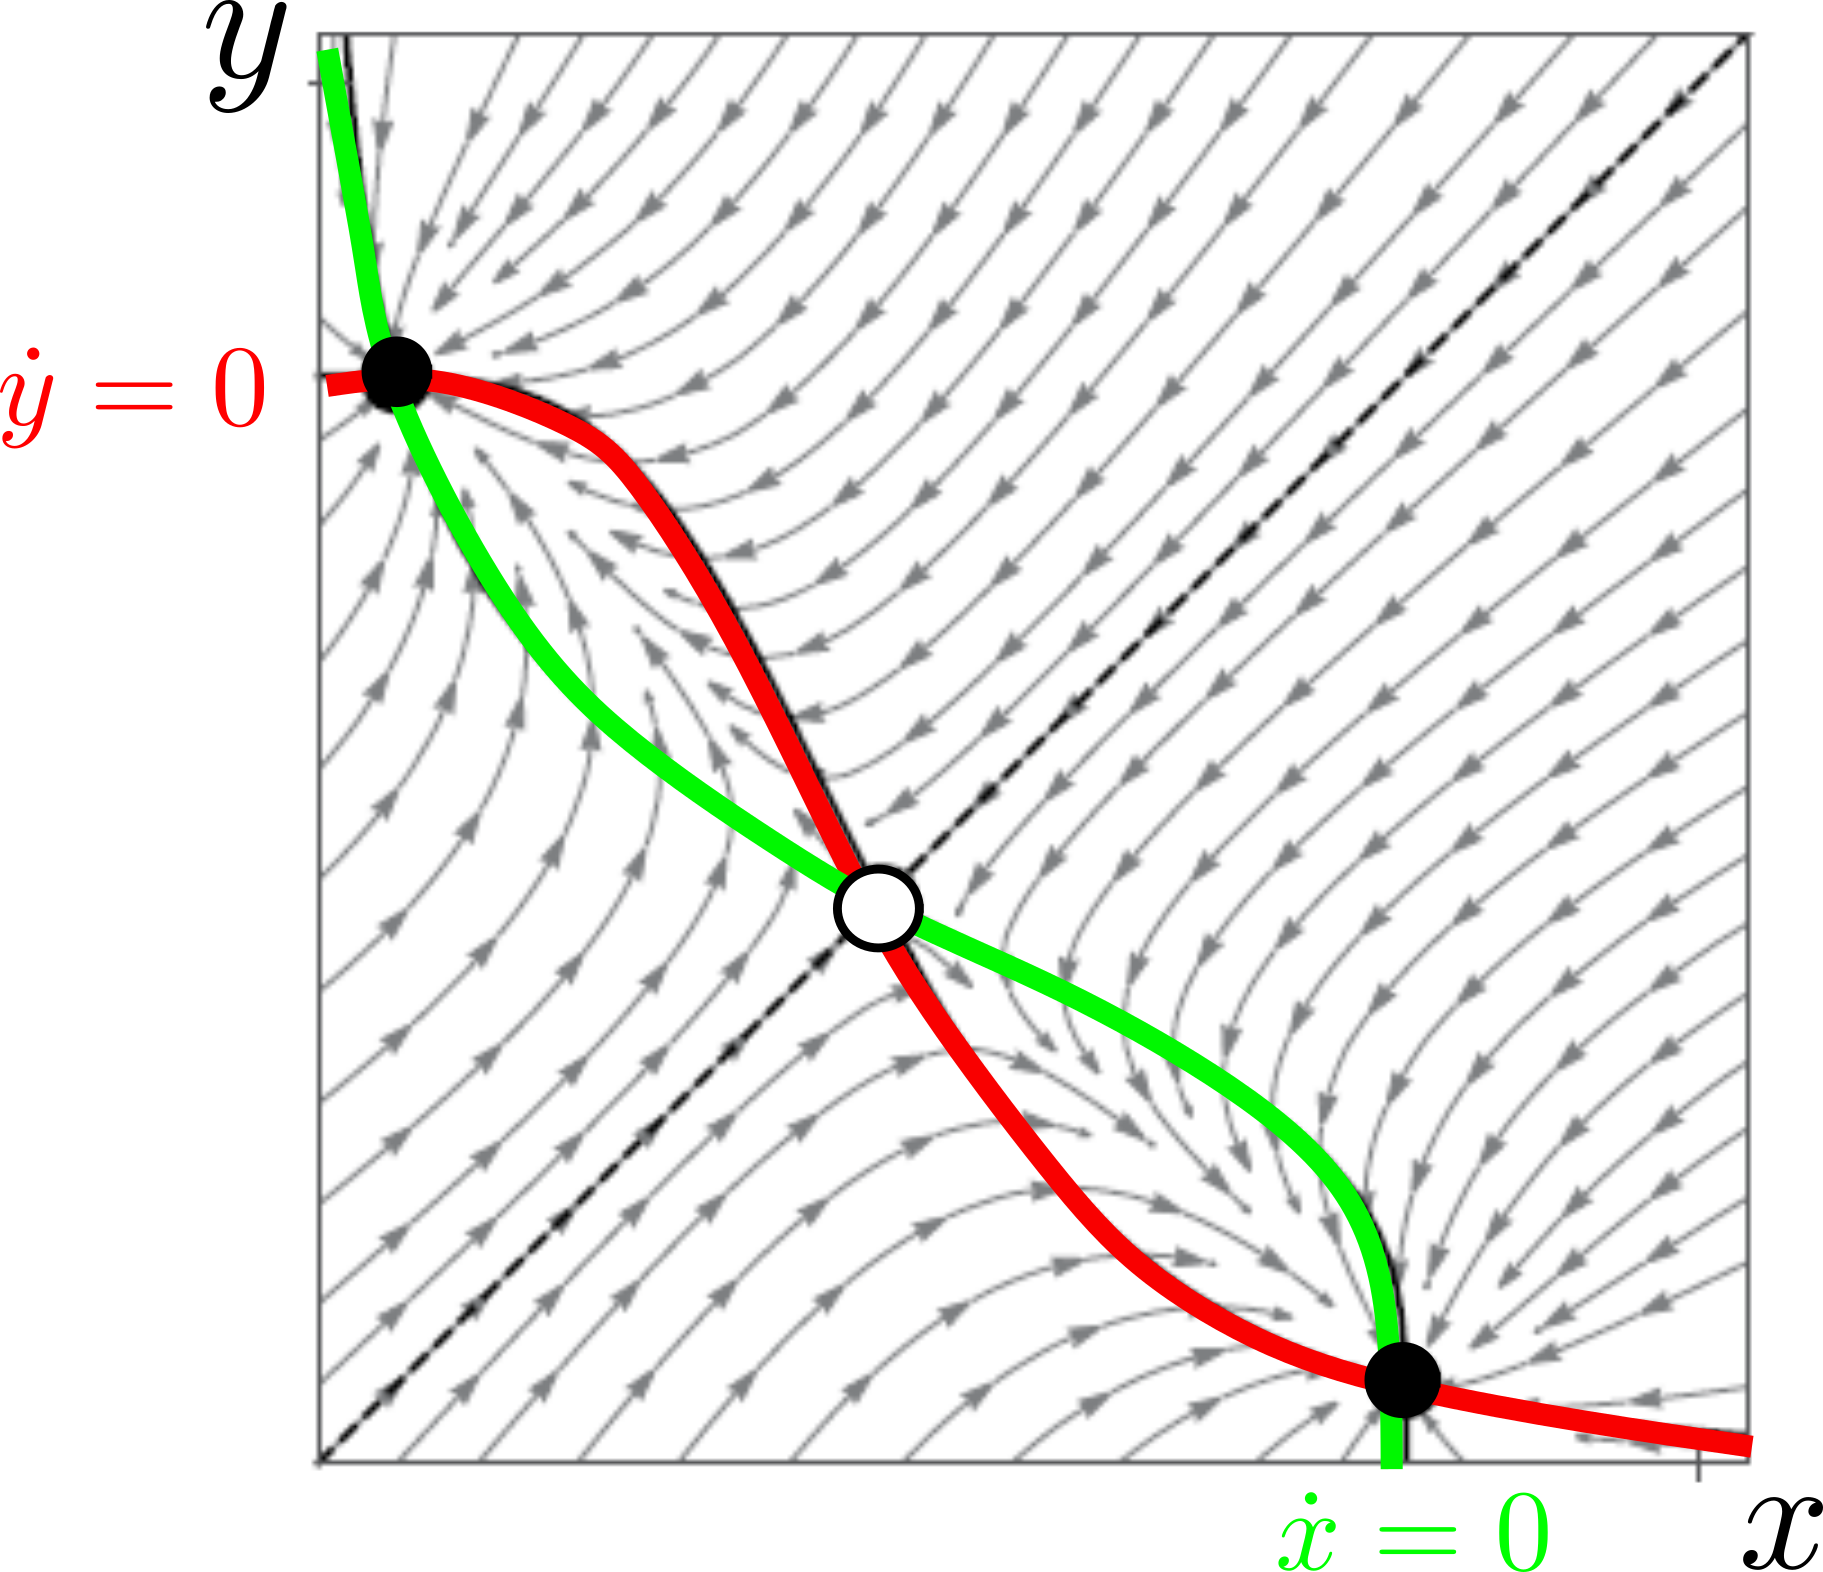
\includegraphics[width=3in]
{autoregulons/2dim-3fp.png}
\caption{Phase portrait
for genetic toggle switch.}
\label{fig-2dim-3fp}
\end{figure}

We can say the system is in the (ON, ON) position
when it's at sink $A$ and $x=x_A$, $y=y_A$.
We can say the system is in the (OFF, OFF) position
when it's at sink $B$ and $x=x_B$, $y=y_B$.
That is why it's referred to as a toggle switch. Note
that the Phase Portrait Fig.\ref{fig-2dim-3fp}
does not describe the system during the transition
from sink $A$ to $B$. During that transition,
the potential function must become shallower in one sink 
than in the other to induce the system to switch sinks.

For simplicity let us consider the large $n_1$ and $n_2$ limit
of the bnet Eq.(\ref{eq-genetic-toggle-hill})

\beq
\begin{array}{ccc}
(a)
&\xymatrix@C=5pc
{\Rect{\rvx}
\fbackar{r}{\redominus}
{\redominus}
&\Rect{\rvy}
}
&
\left\{
\begin{array}{l}
\dot{x}=-\alp_1 x + \beta_1\indi(y<K_{y\rarrow x})
\\
\dot{y}= -\alp_2y + \beta_2\indi(x<K_{x\rarrow y})
\end{array}
\right.
\\
\\
(b)&
\xymatrix@C=5pc
{\Rect{\rvx}
\fbackar{r}{\redoplus}
{\redoplus}
&\Rect{\rvy}
}
&
\left\{
\begin{array}{l}
\dot{x}=-\alp_1 x + \beta_1 \indi(y>K_{y\rarrow x})
\\
\dot{y}= -\alp_2y + \beta_2 \indi(x>K_{x\rarrow y})
\end{array}
\right.
\end{array}
\label{eq-genetic-toggle-steps}
\eeq
Define

\beq
x_\infty=\frac{\beta_1}{\alp_1}\;,\;\;
y_\infty=\frac{\beta_2}{\alp_2}
\eeq
Define $x=x_\infty$ as ON, and $x=0$ as OFF. Same for $y$.

\begin{figure}[h!]
\centering
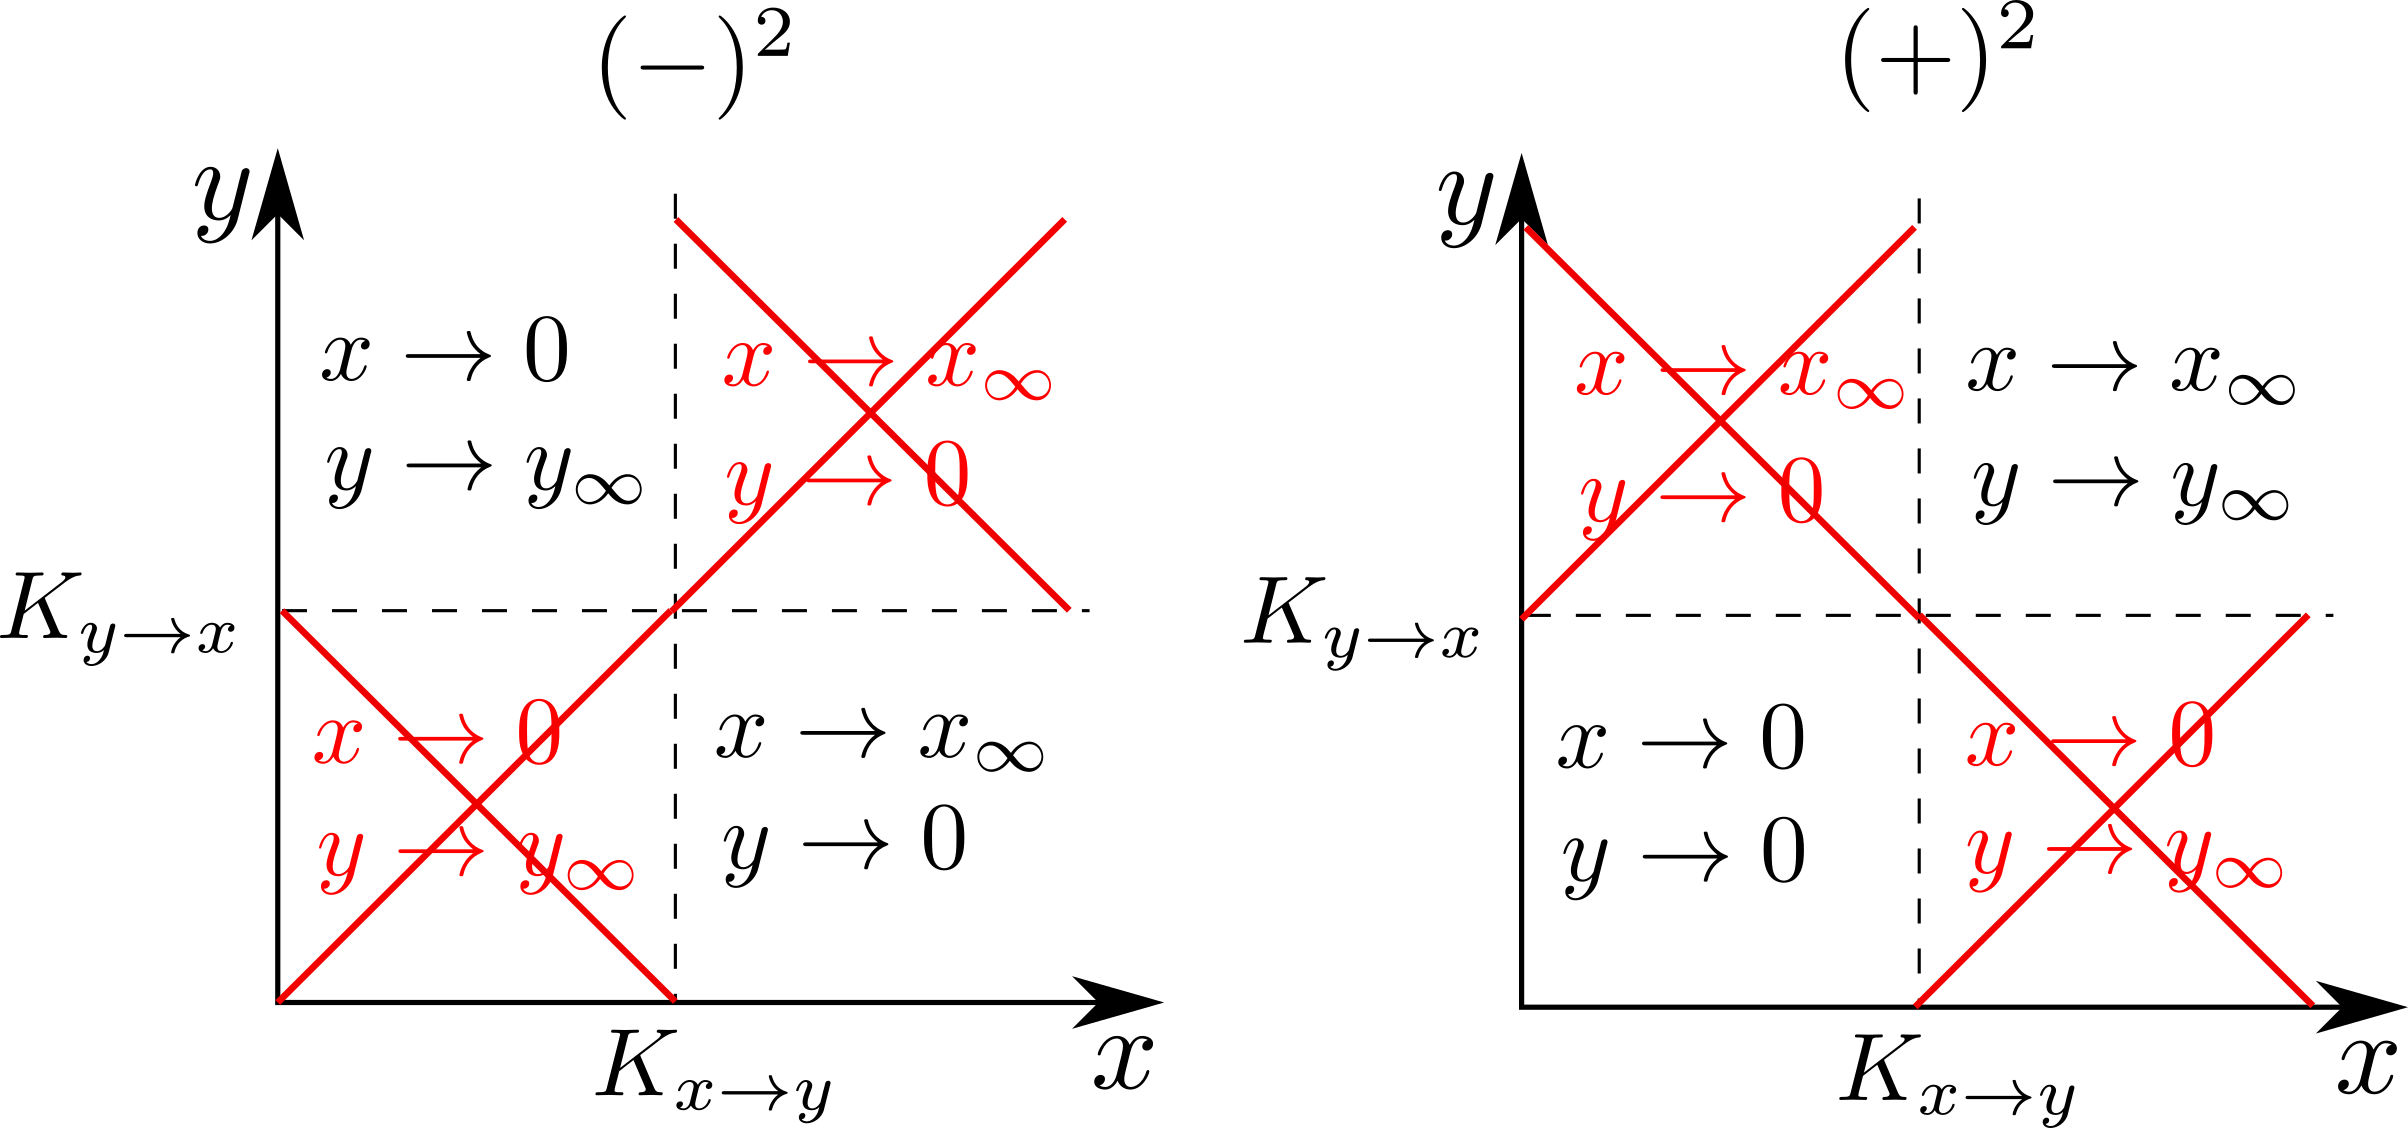
\includegraphics[width=4in]
{autoregulons/double-plus-minus-tables.png}
\caption{Steady state behavior tables for $(-)^2$ and $(+)^2$ feedback loop nets. 
The red, crossed out entries are untenable.}
\label{fig-double-plus-minus-tables}
\end{figure}

It's easy to conclude from our knowledge
of the general solution to the autoregulon ODE, that the table
Fig.\ref{fig-double-plus-minus-tables}
correctly describes the steady state 
(i.e., $t\rarrow \infty$ limit) of 
the system Eq.(\ref{eq-genetic-toggle-steps}).





\section{More than 2 autoregulons}

\subsection{$(-)^2$ and $(+)^2$ Regulator nets}
One can add an extra autoregulon to the
 $(-)^2$ and $(+)^2$ bnets considered above.
 When the autoregulon $\rvz$
 acts as a common cause
 of the two autoregulons 
 $\rvx, \rvy$, we will call it 
 a {\bf regulated $(-)^2$ or $(+)^2$}  bnet.
 When $z$ acts instead as a common effect,
 we will call it a {\bf $(-)^2$ or $(+)^2$ regulator}
 bnet.
 
 In this section, we consider the following
 bnets, which we call the {\bf $(-)^2$ and $(+)^2$ regulator}
  bnets:

\beq
\begin{array}{ccc}
(a)
&\xymatrix
{\Rect{\rvx}
\fbackar{rr}{\redominus}
{\redominus}
\ar[dr]|\redominus
&&\Rect{\rvy}
\ar[dl]|\redoplus
\\
&\bigoplus\ar[d]
\\
&\Rect{\rvz}
}
&
\left\{
\begin{array}{l}
\dot{x}=-\alp_1 x + \beta_1\indi(y<K_{y\rarrow x})
\\
\dot{y}= -\alp_2y + \beta_2\indi(x<K_{x\rarrow y})
\\
\dot{z}= -\alp_3 z + \beta_3
\indi(x<K_{x\rarrow y})
\indi(y>K_{y\rarrow x})
\end{array}
\right.
\\
\\
(b)&
\xymatrix
{\Rect{\rvx}
\fbackar{rr}{\redoplus}
{\redoplus}
\ar[dr]|\redoplus
&&\Rect{\rvy}
\ar[dl]|\redoplus
\\
&\bigoplus\ar[d]
\\
&\Rect{\rvz}
}
&
\left\{
\begin{array}{l}
\dot{x}=-\alp_1 x + \beta_1 \indi(y>K_{y\rarrow x})
\\
\dot{y}= -\alp_2y + \beta_2 \indi(x>K_{x\rarrow y})
\\
\dot{z}= -\alp_3 z + \beta_3
\indi(x>K_{x\rarrow y})
\indi(y>K_{y\rarrow x})
\end{array}
\right.
\end{array}
\label{eq-z-regulator}
\eeq
Define
\beq
x_\infty=\frac{\beta_1}{\alp_1}\;,\;\;
y_\infty=\frac{\beta_2}{\alp_2}\;,\;\;
z_\infty=\frac{\beta_3}{\alp_3}
\eeq
 Define $x=x_\infty$ as ON,
 and $x=0$ as OFF. Same for $y$ and $z$.


\begin{figure}[h!]
\centering
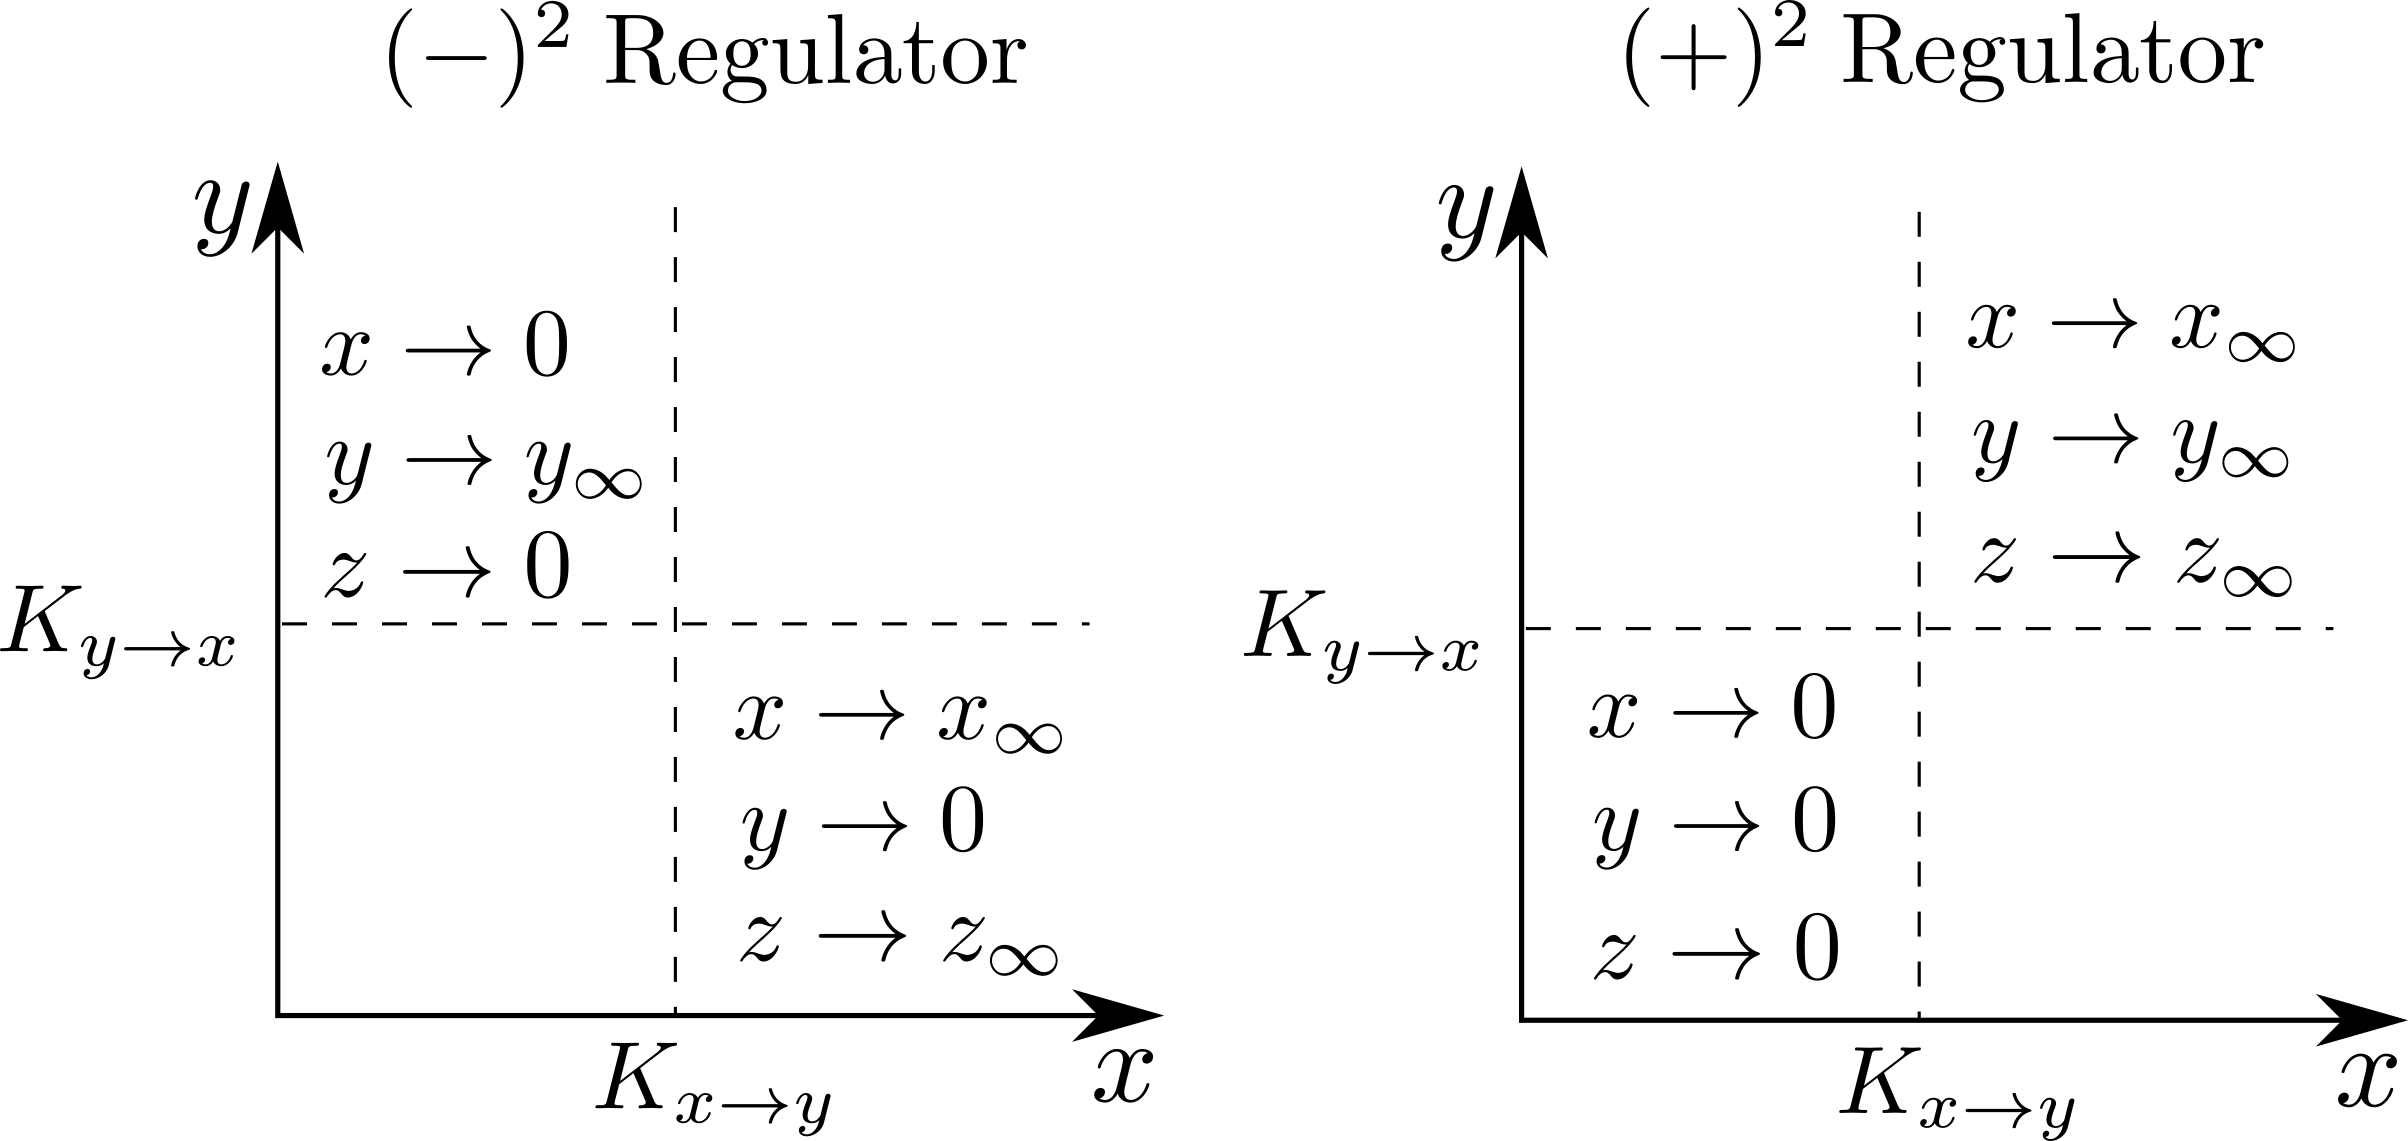
\includegraphics[width=4in]
{autoregulons/reg-double-plus-minus-tables.png}
\caption{Steady state behavior tables for $(-)^2$ and $(+)^2$ regulator nets.
This figure is based on Fig.\ref{fig-double-plus-minus-tables} }
\label{fig-reg-double-plus-minus-tables}
\end{figure}
It's easy to conclude from our knowledge
of the general solution to the autoregulon ODE, that the table
Fig.\ref{fig-reg-double-plus-minus-tables}
correctly describes the steady state 
(i.e., $t\rarrow \infty$ limit) of 
the system Eq.(\ref{eq-z-regulator}).

\newpage
\subsection{Regulated $(-)^2$ and $(+)^2$ nets}

In this section, we consider the following
 bnets, which we call the {\bf regulated  $(-)^2$ and $(+)^2$}
  bnets:

\beq
\begin{array}{ccc}
(a)
&\xymatrix
{
&\Rect{\rvz}
\ar[dl]|\redminus
\ar[dr]|\redplus
\\
\Rect{\rvx}
\fbackar{rr}{\redominus}
{\redominus}
&&\Rect{\rvy}
}
&
\left\{
\begin{array}{l}
\dot{x}=-\alp_1 x 
- \gamma z
+ \beta_1\indi(y<K_{y\rarrow x})
\\
\dot{y}= -\alp_2y 
+ \gamma z
+ \beta_2\indi(x<K_{x\rarrow y})
\end{array}
\right.
\\
\\
(b)&
\xymatrix
{
&\Rect{\rvz}
\ar[dl]|\redplus
\ar[dr]|\redplus
\\
\Rect{\rvx}
\fbackar{rr}{\redoplus}
{\redoplus}
&&\Rect{\rvy}
}
&
\left\{
\begin{array}{l}
\dot{x}=-\alp_1 x 
+ \gamma z
+ \beta_1 \indi(y>K_{y\rarrow x})
\\
\dot{y}= -\alp_2y 
+ \gamma z
+ \beta_2 \indi(x>K_{x\rarrow y})
\end{array}
\right.
\end{array}
\label{eq-plots-regulated-double-sign}
\eeq

\begin{figure}[h!]
\centering
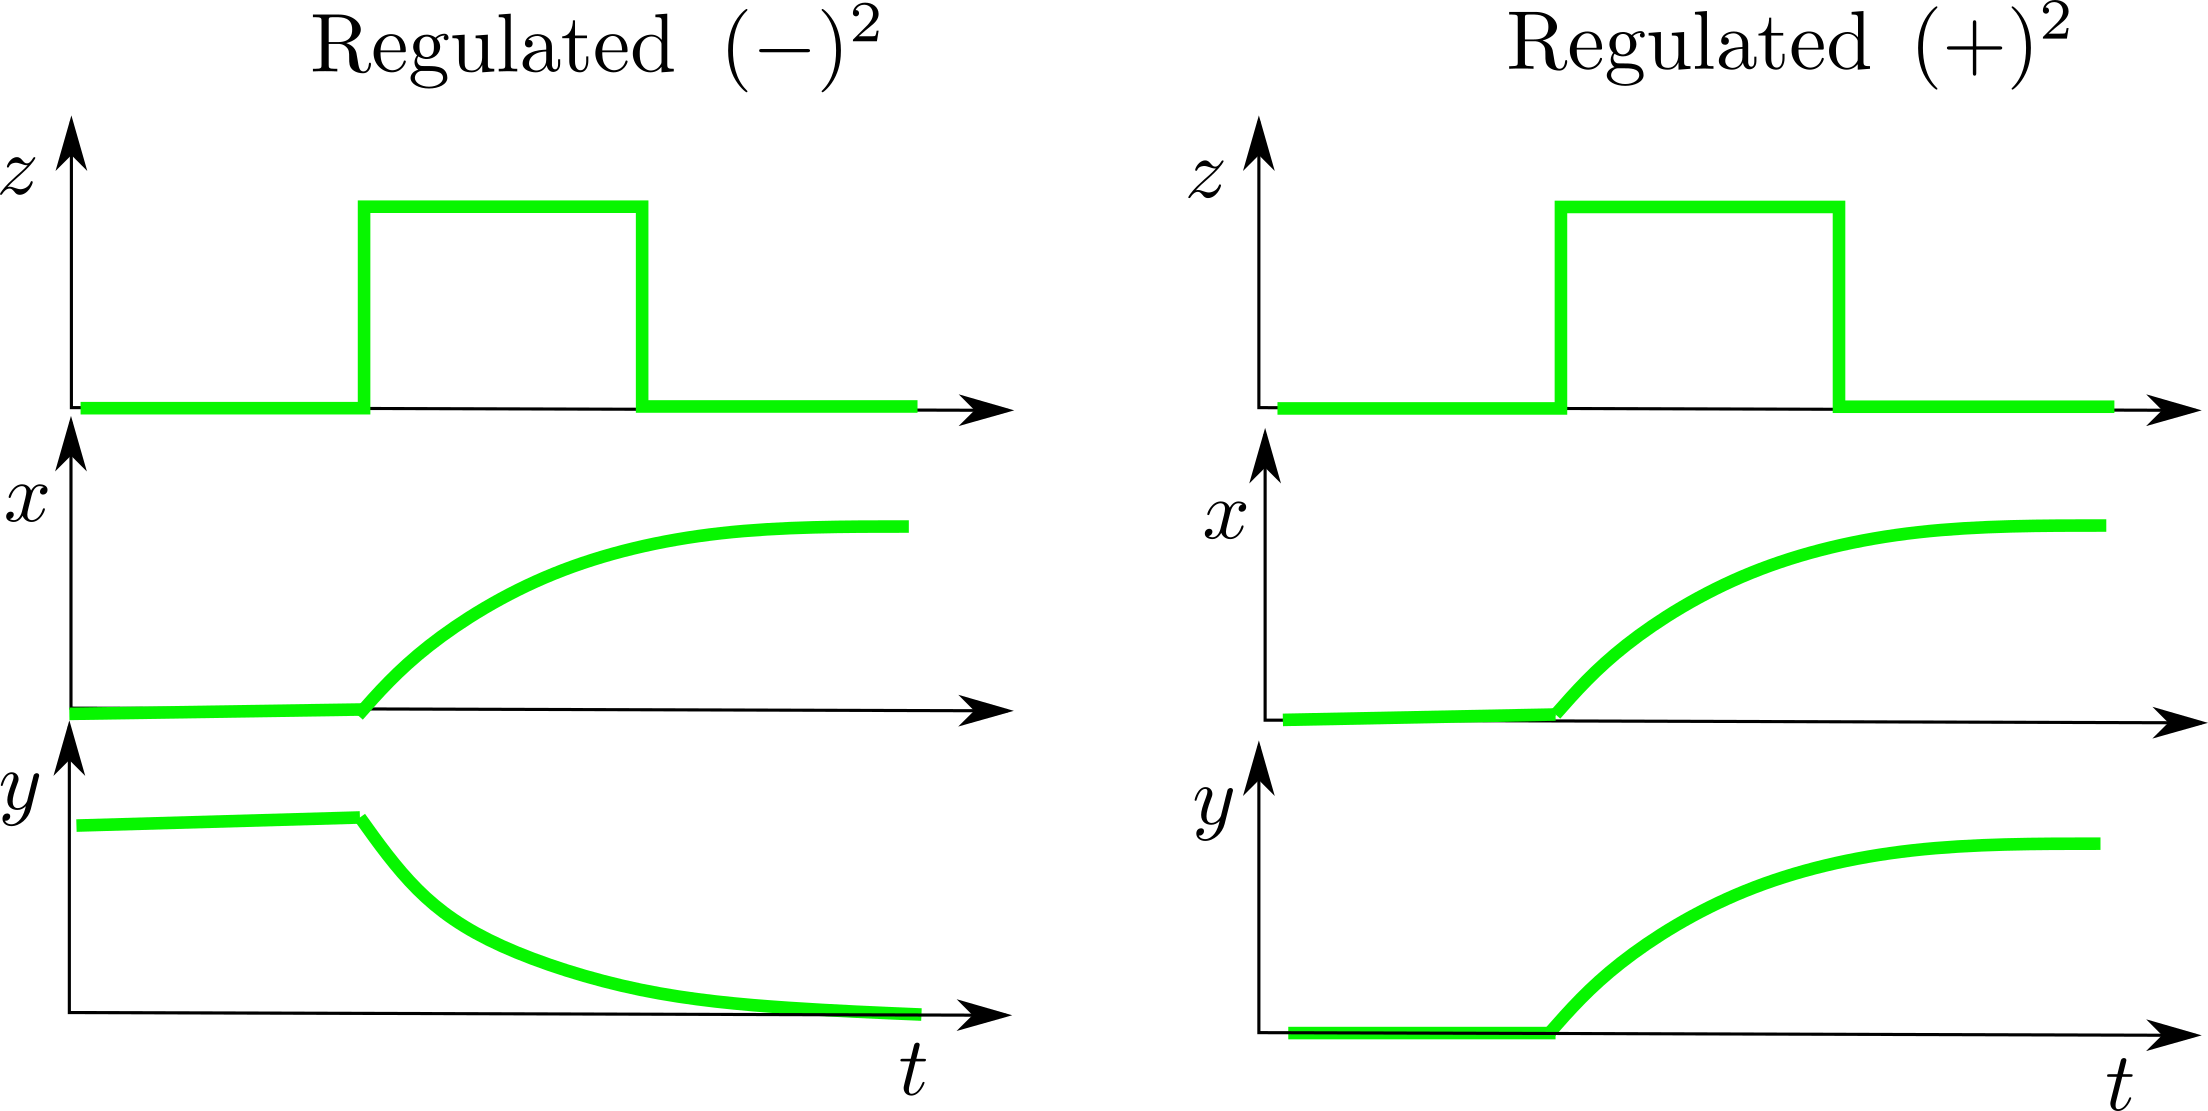
\includegraphics[width=3.9in]
{autoregulons/confounded-plus-minus-plots.png}
\caption{$z(t), x(t), y(t)$ plots for regulated $(-)^2$ and $(+)^2$ nets.}
\label{fig-confounded-plus-minus-plots.png}
\end{figure}
Fig.\ref{fig-confounded-plus-minus-plots.png}
shows the response of system Eq.(\ref{eq-plots-regulated-double-sign}) to
a pulse coming from the common cause $\rvz$.
The pulse can jolt the 
system from
one sink to the other.


\subsection{Feed Forward Loops}


The most general 3 autoregulon bnet is this

\beq
\xymatrix@C=3pc@R=5pc{
&\Rect{\rvx}
\fbackar{ld}{}{}
\fbackar{rd}{}{}
\\
\Rect{\rvy}\fbackar{rr}{}{}
&&
\Rect{\rvz}
}
\quad
\left\{
\begin{array}{l}
\dot{x}= f_1(x) +
\gamma_{y\rarrow x} y + 
\gamma_{z\rarrow x} z
\\
\dot{y} = f_2(y) + 
\gamma_{x\rarrow y} x + 
\gamma_{z\rarrow y} z
\\
\dot{z} = f_3(z) + 
\gamma_{x\rarrow z} x + 
\gamma_{y\rarrow z} y
\end{array}
\right.
\eeq
We will call a {\bf feed forward loop} (FFL) 
any 
 3 autoregulon
net which has only one arrow 
between each pair of nodes,
and the 3 arrows form an acyclic net.
FFLs can be classified into
coherent and incoherent.
A {\bf coherent FFL} is an FFL
for which the product of
the signs of its arrows is positive.
For an {\bf incoherent FFL},
that product is negative.
See Fig.\ref{fig-3-coherent-autoregulons}
for examples of coherent and incoherent FFL.


\begin{figure}[h!]
$$
\begin{array}{cccccc}
\xymatrix@C=1.8pc@R=5pc{
&\Rect{\rvx}
\fbackar{ld}{-}{0}
\fbackar{rd}{+}{0}
\\
\Rect{\rvy}\fbackar{rr}{-}{0}
&&
\Rect{\rvz}
}&=
&
\xymatrix@C=1pc{
&\Rect{\rvx}
\ar[ld]|\redminus
\ar[rd]|\redplus
\\
\Rect{\rvy}\ar[rr]|\redminus
&&
\Rect{\rvz}
}
&
\xymatrix@C=1.8pc@R=5pc{
&\Rect{\rvx}
\fbackar{ld}{-}{0}
\fbackar{rd}{-}{0}
\\
\Rect{\rvy}\fbackar{rr}{-}{0}
&&
\Rect{\rvz}
}&=
&
\xymatrix@C=1pc{
&\Rect{\rvx}
\ar[ld]|\redminus
\ar[rd]|\redminus
\\
\Rect{\rvy}\ar[rr]|\redminus
&&
\Rect{\rvz}
}
\\
\\
&(a)&&&(b)
\end{array}
$$
\caption{$(a)$ is a coherent FFL 
 because the product of the signs of its arrows is $+$.
$(b)$ is an incoherent FFL because because the product of the signs of its arrows is $-$.
The $+$'s can be changed to $\oplus$'s and
the $-$'s to $\ominus$'s.
}
\label{fig-3-coherent-autoregulons}
\end{figure}

\begin{figure}
$$
\begin{array}{cc}
\xymatrix{
&\Rect{\rvx}\ar[dl]|\redoplus
\ar[dr]|\redoplus
\\
\Rect{\rvy}\ar[rr]|\redoplus
&&\Rect{\rvz}
}
&
\xymatrix{
&\Rect{\rvx}\ar[dl]|\redoplus
\ar[dr]|\redominus
\\
\Rect{\rvy}\ar[rr]|\redoplus
&&\Rect{\rvz}
}
\\
(a)
&(b)
\end{array}
$$
\caption{
$(a)$ Coherent Type 1 FFL (C1-FFL).
$(b)$ Incoherent Type 1 FFL (I1-FFL)}
\label{fig-c1-ffl-inco1-ffl}
\end{figure}


We will
also refer to the following bnet
as either a CI-FFL or an I1-FFL,
depending on whether $h_? =h_\oplus$ (coherent)
or   $h_? =h_\ominus$ (incoherent):

\beq
\xymatrix@R=1pc{
&&\Rect{\rvx}
\ar@/_1pc/[ddll]|\redoplus
\ar[dl]|{\color{red} ?}
\\
&\bigotimes
\ar@/_1pc/[drr]
\\
\Rect{\rvy}\ar[ur]|\redoplus
&&&\Rect{\rvz}
}
\quad
\left\{
\begin{array}{l}
\dot{x}= f_1(x)
\\
\dot{y} = f_2(y) + \beta_2
h_\oplus(x)
\\
\dot{z} = f_3(z) + 
h_\oplus(x)h_?(y)
\end{array}
\right.
\label{eq-ffl-and-gate}
\eeq

Note that if
in the net of Eq.(\ref{eq-ffl-and-gate}),
the product $\bigotimes$
gate (representing an AND gate) is
replaced by a sum $\bigoplus$ gate (representing an OR gate),  then the
net of Eq.(\ref{eq-ffl-and-gate}) becomes 
Fig.\ref{fig-c1-ffl-inco1-ffl}.
Both the bnets with $\bigotimes$ and
$\bigoplus$ are referred to as FFL.


\subsection{C1-FFL}

\beq
\xymatrix{
\rvx \ar@/_1pc/[drr]|\redoplus
\ar[r]|\redoplus
&\bigotimes\ar@/_3pc/[drr]|{\redplus}
& \rvy\ar[d]|{\redminus}\ar[l]|
\redoplus
&\rvz\ar[d]|{\redminus}
\ar@/_1pc/[d]|\redominus
\\
\ar[u]
&
& \dot{y}
&
\dot{z} 
}
\left\{
\begin{array}{l}
\dot{y} = -\alp_2 y + \beta_2 
\indi(x>K_{x\rarrow y})
\\
\dot{z} = -\alp_3 z + \beta_3\indi(z<K_3)+
\beta_{12} \indi(x> K_{x\rarrow z})
\ul{\indi(y>K_{y\rarrow z})}
\end{array}
\right.
\label{eq-c1-ffl-simp}
\eeq
The underlined term in 
Eq.(\ref{eq-c1-ffl-simp})
is the only
difference between the
ODEs for this
C1-FFL, and 
the ODEs Eq.(\ref{eq-inc1-ffl-simp})
for an I1-FFL.


\begin{figure}[h!]
\centering
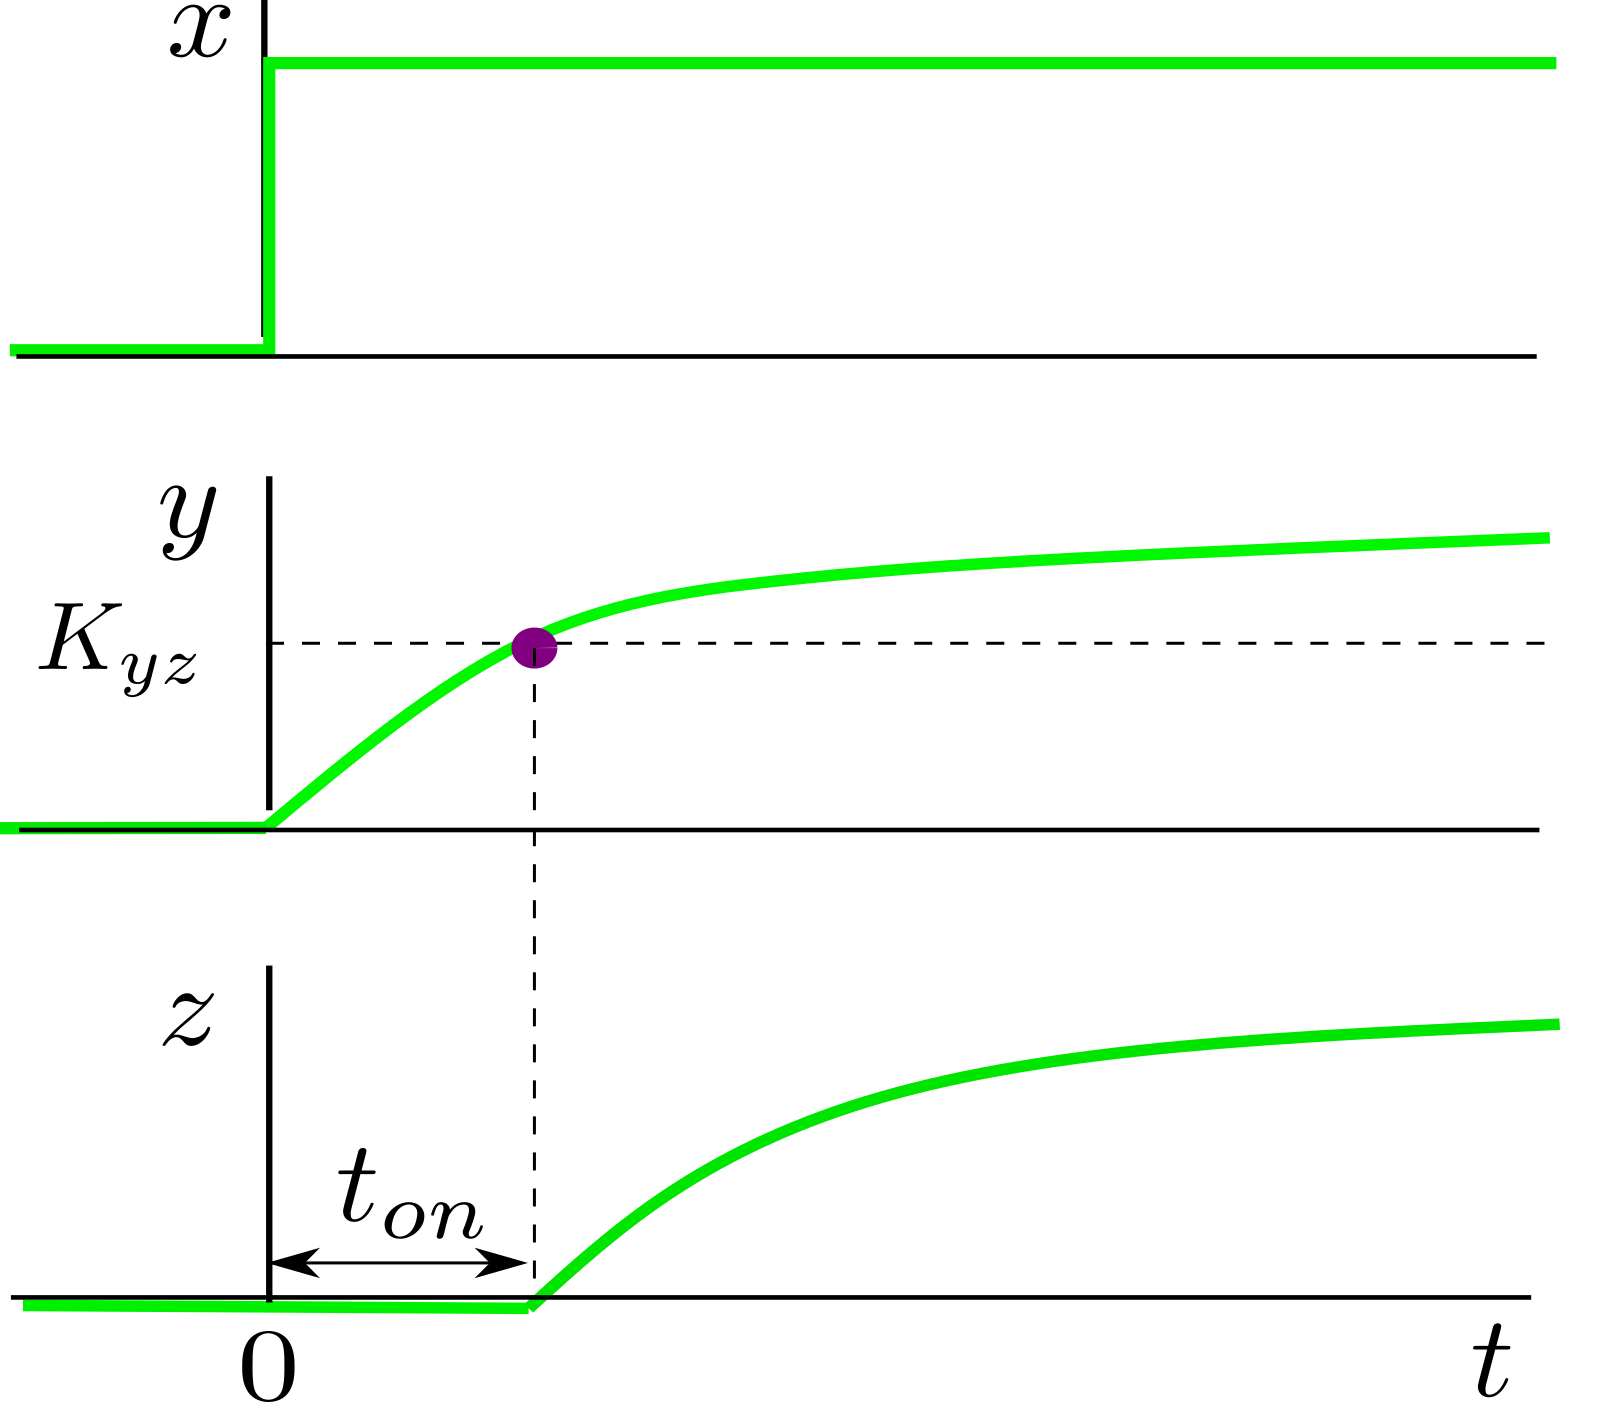
\includegraphics[height=2in]
{autoregulons/c1-ffl-up-green.png}
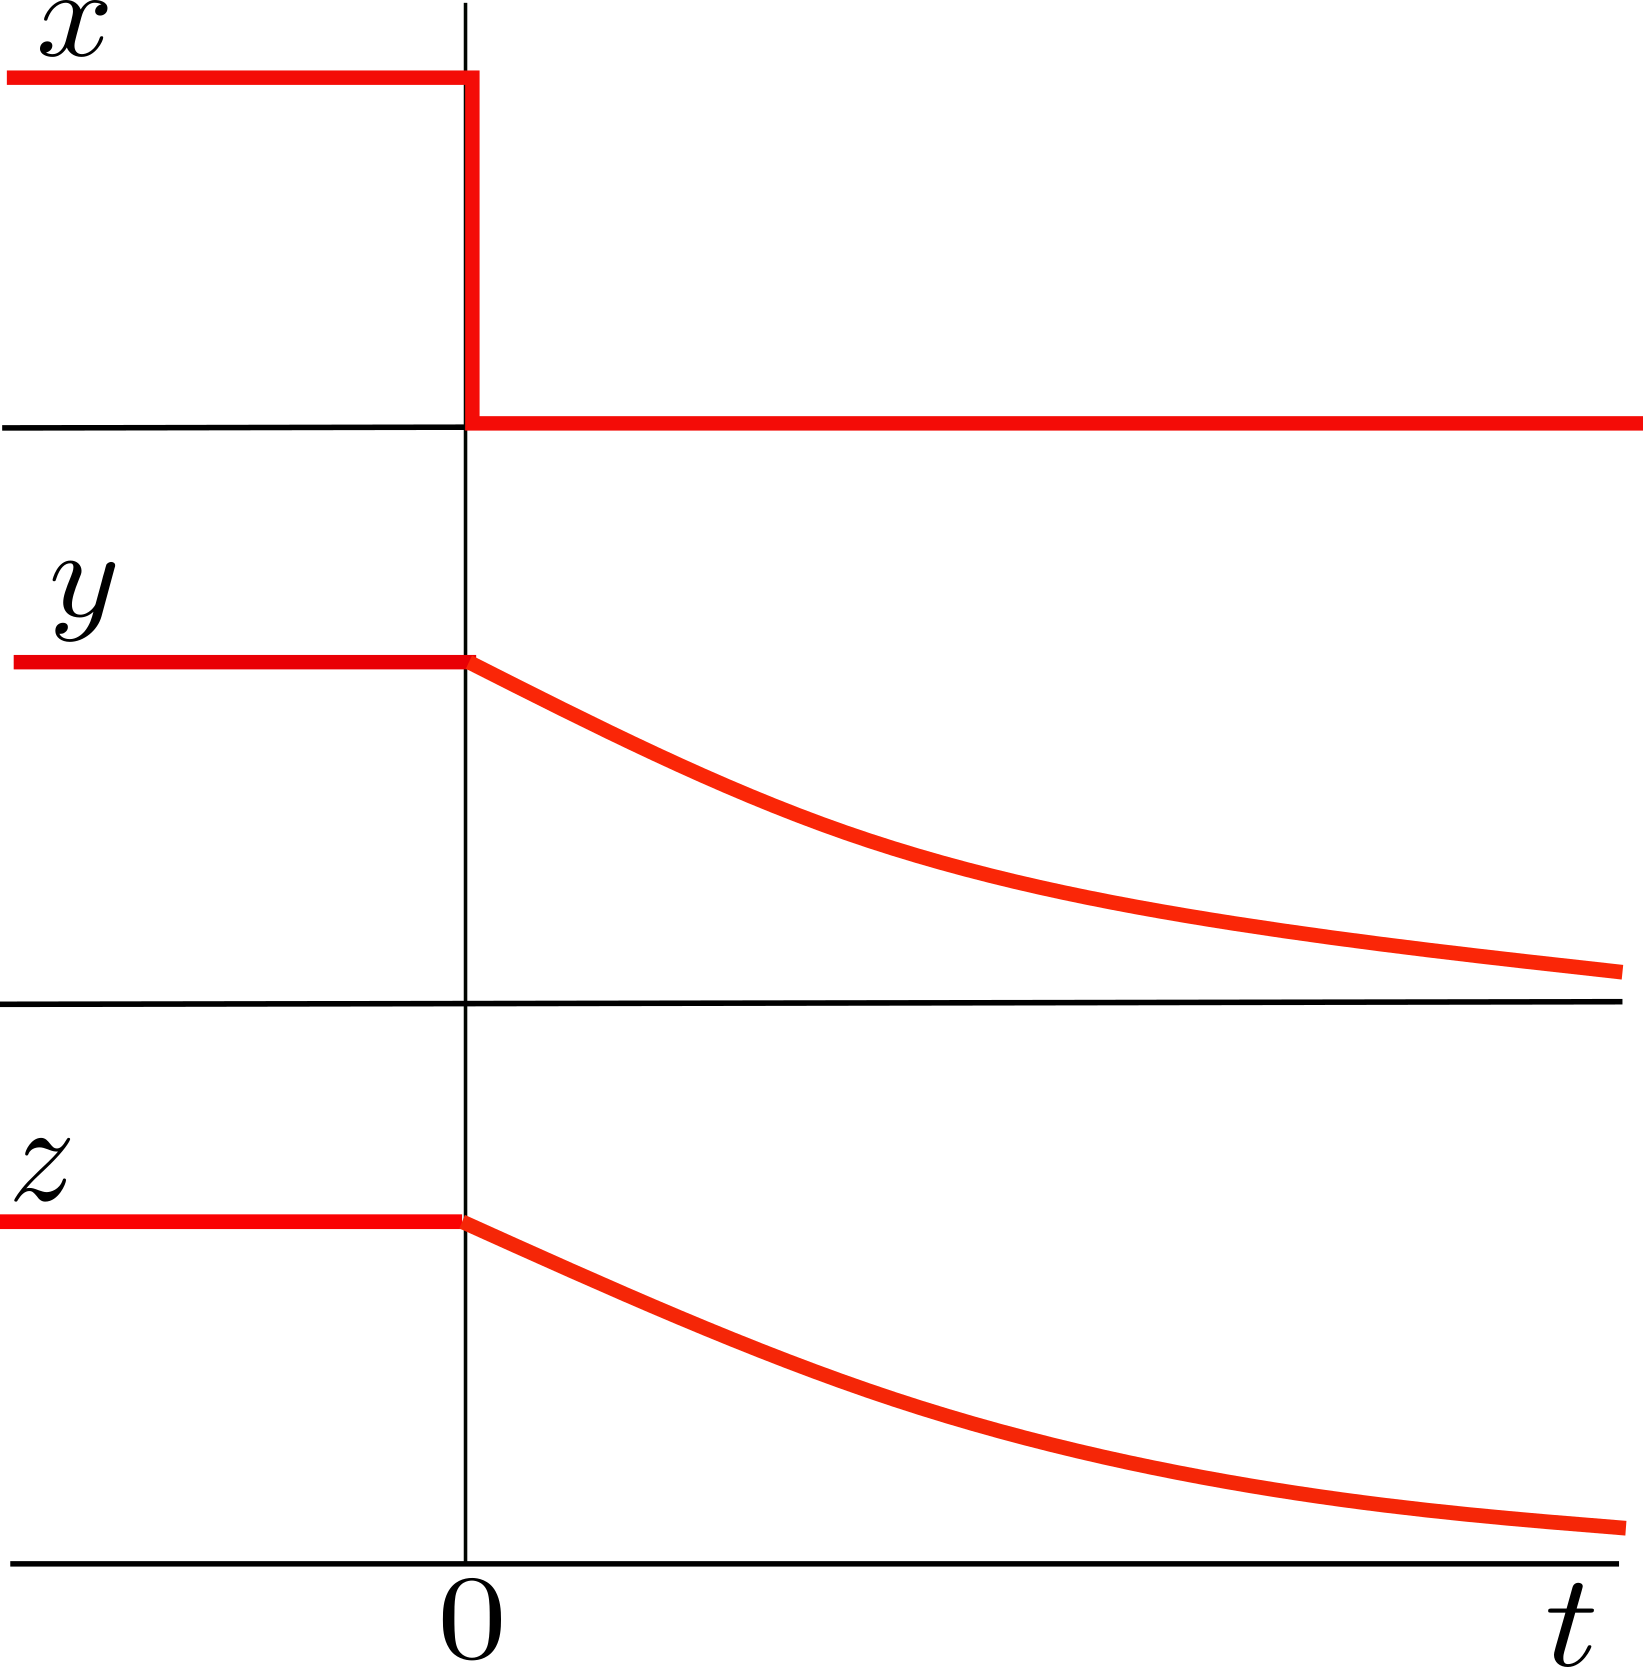
\includegraphics[height=2in]
{autoregulons/c1-ffl-down-green.png}
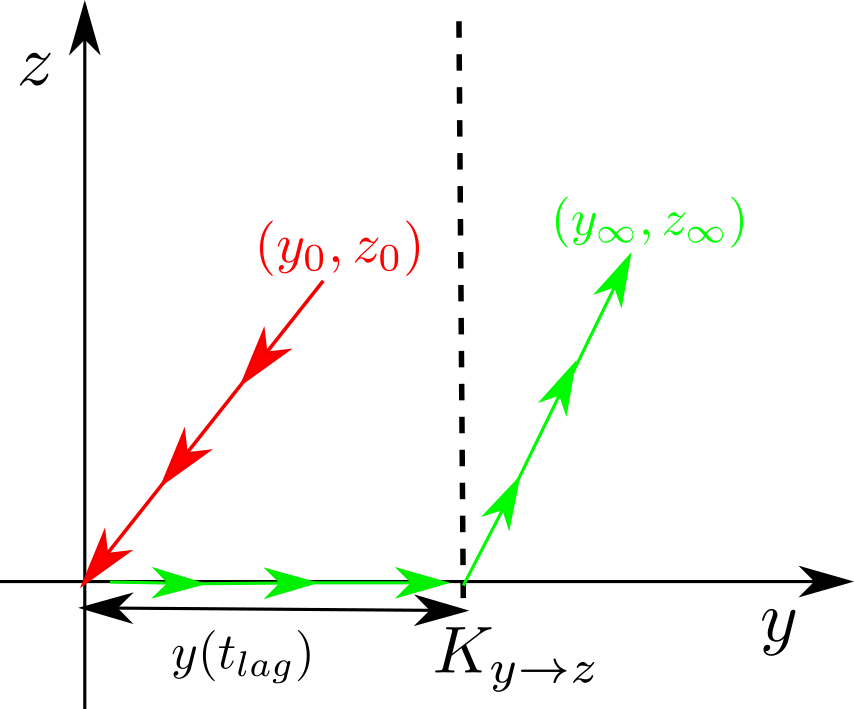
\includegraphics[height=2in]
{autoregulons/two-paths-y-z-plane.png}
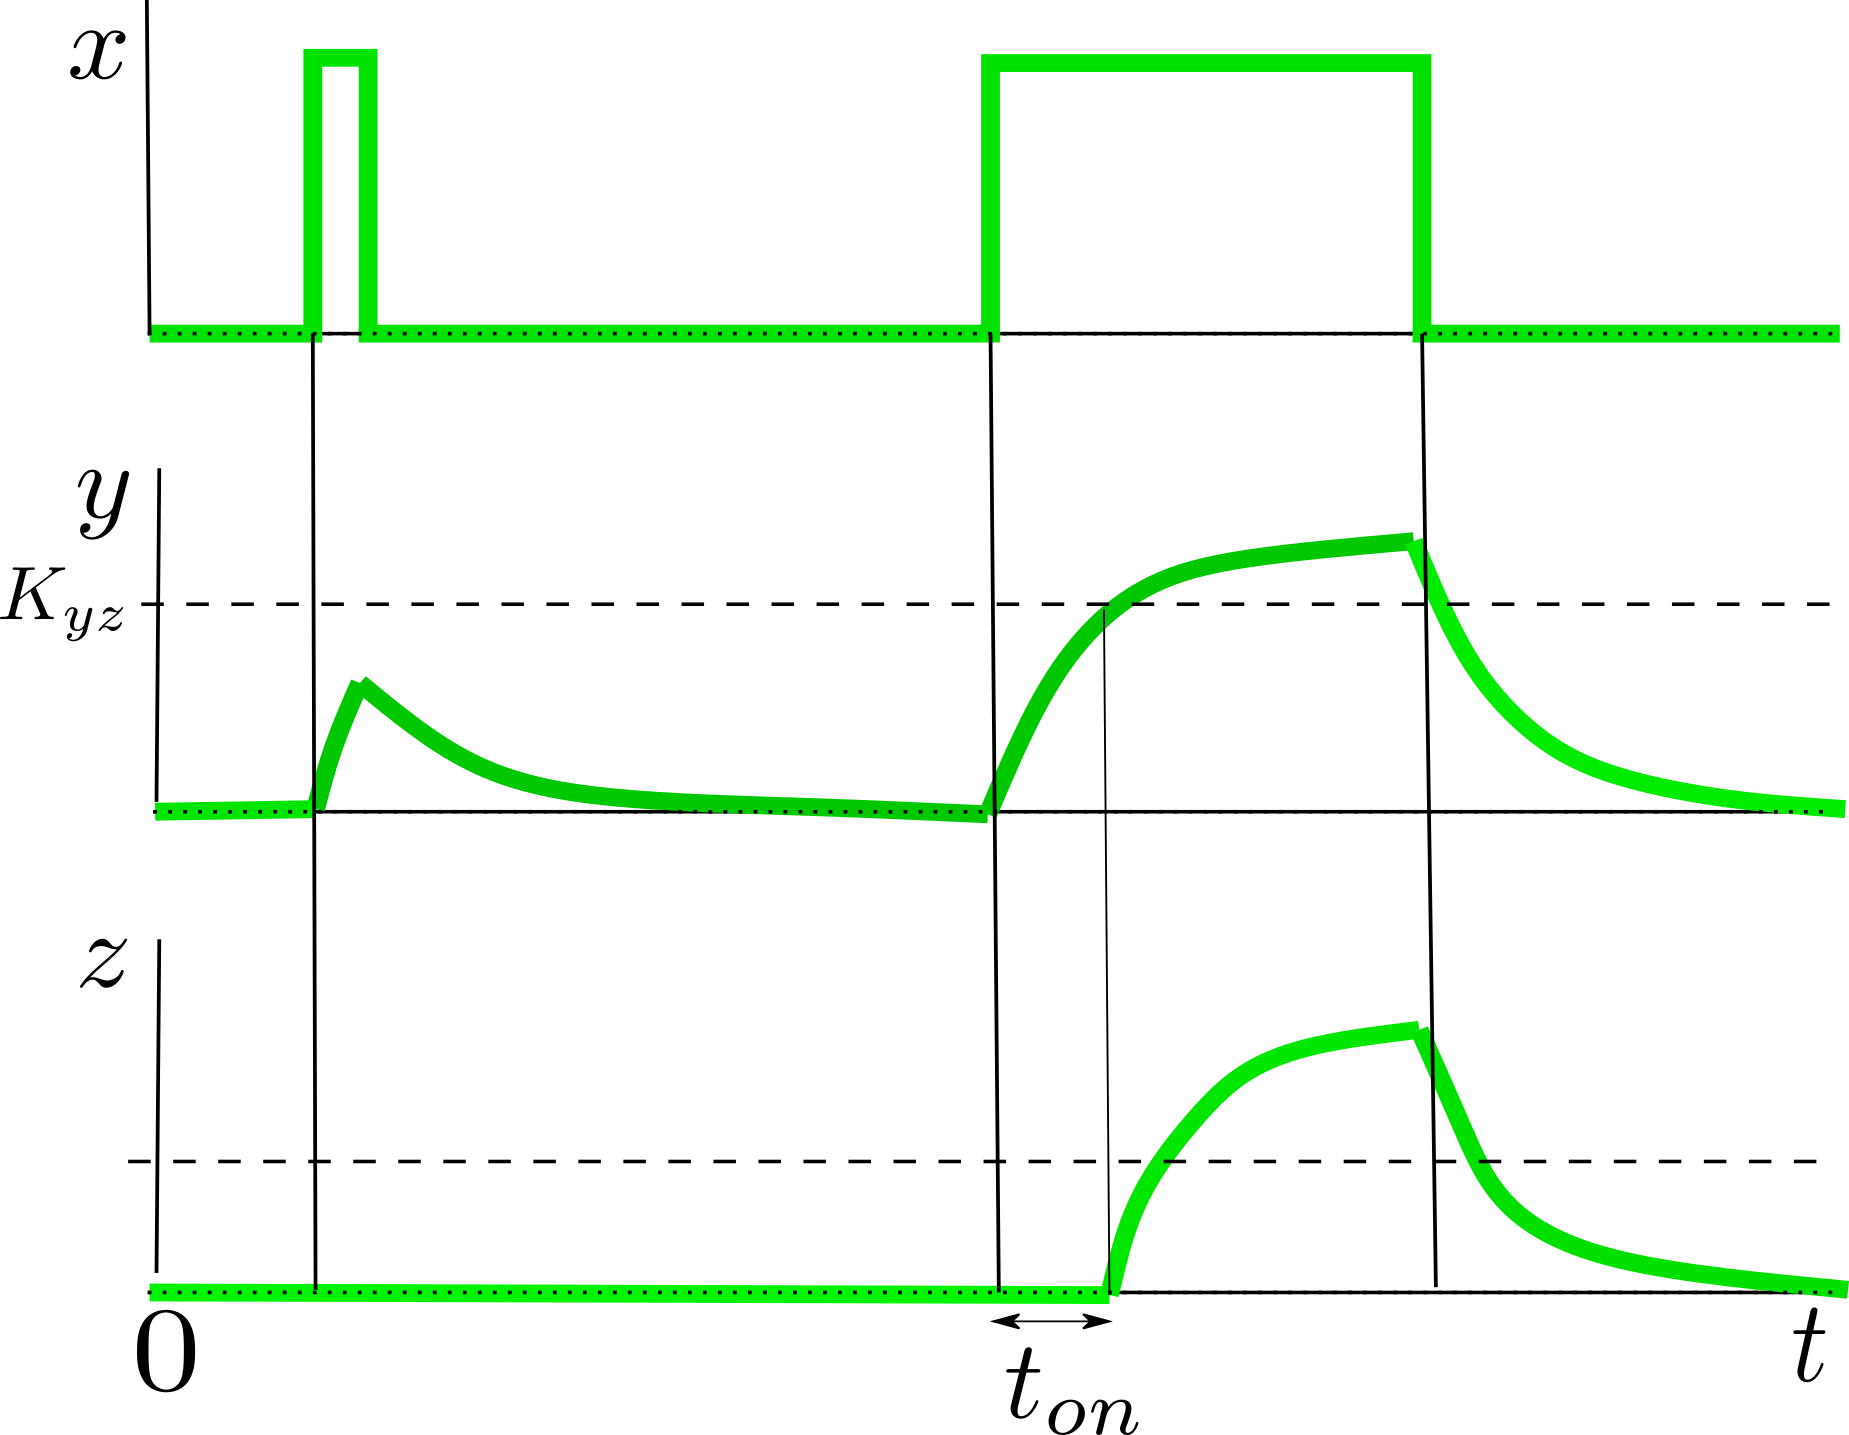
\includegraphics[height=2in]
{autoregulons/c1-ffl-up-down-green.png}
\caption{For C1-FFL, $x(t)$, $y(t)$, $z(t)$ assuming 
that $x(t)$ is either a rising
 t-step function (in green),
a dropping t-step function (in red),
or a t-pulse  (in purple).}
\label{fig-c1-ffl-triple}
\end{figure}

See Fig.\ref{fig-c1-ffl-triple}
for a pictorial
representation of
what we will prove in this section.

We will assume $z<K_3$ always so $\indi(z<K_3)=1$.

\beq
x = 
\left\{
\begin{array}{ll}
\xi \indi(t>0)
& \text{if $x$ up t-step}
\\
\xi \indi(t<0)
& \text{if $x$ down t-step}
\end{array}
\right.
\eeq
From the
solution for $z(t)$
for these 2 cases of $x(t)$ 
equal to a
up and a down t-step, 
we will infer the solution
for $x(t)$ equal to a 
a t-pulse:

\beq
x=\xi \indi_{t_1}^{t_2}(t)
\eeq

Let $\xi  >
\max(K_{x\rarrow y}, K_{x\rarrow z})$.
Thus, Eq.(\ref{eq-c1-ffl-simp}) reduces to

\beq
\left\{
\begin{array}{l}
\dot{y} = -\alp_2 y +\beta_2
\\
\dot{z} = -\alp_3 z+ \beta_3 + \beta_{12}
\indi(y>K_{y\rarrow z}) 
\end{array}
\right.
\label{eq-ffl-red}
\eeq
Let 

\beq
y_\infty = \frac{\beta_2}{\alp_2}\;,\;\;
z_\infty = \frac{\beta_3}{\alp_3}\;,\;\;
z_\infty' = \frac{\beta_3 + \beta_{12}}{\alp_3}
\eeq
Then 

\beq
y =
\left\{
\begin{array} {ll}
y_\infty(1-e^{-\alp_2 t})
& \text{if $x$ up step, $y(0)=0$}
\\
y_0e^{-\alp_2 t}
& \text{if $x$ down step, $y(0)=y_0$}
\end{array}
\right.
\eeq
and


\beq
z=
\left\{
\begin{array}{ll}
z_\infty'(1- e^{-\alp_3 (t-t_{lag})})
&
\text{if $x$ up step,
$y(0)=0$, $y> K_{y\rarrow z}$}
\\
z_0 e^{-\alp_3 t}
& \text{if $x$ down step, $y(0)=y_0$, $y< K_{y\rarrow z}$
}
\end{array}
\right.
\eeq
where $t_{lag}$ is defined so that

\beq
y(t_{lag}) = K_{y\rarrow z}= y_\infty(1-e^{-\alp_2 t_{lag}})
\eeq
Solving the last equation for $t_{lag}$ yields (see 
Fig.\ref{fig-minus-log-1-minus-x.png})

\beq
t_{lag} = -\;\frac{1}{\alp_2}
\ln
\left({1- \frac{K_{y\rarrow z}}{y_\infty}}
\right)
\eeq

\begin{figure}[h!]
\centering
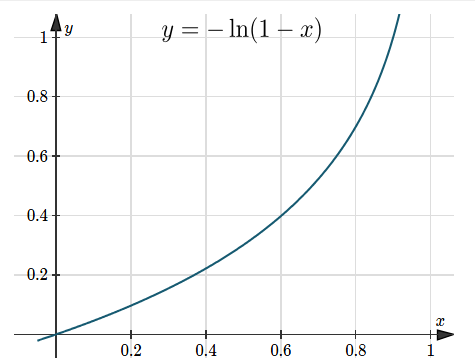
\includegraphics[width=2.8in]
{autoregulons/-log(1-x).png}
\caption{Plot of $y=-\ln(1-x)$.}
\label{fig-minus-log-1-minus-x.png}
\end{figure}

Fig.\ref{fig-c1-ffl-triple}
shows the waveforms for $x(t), y(t), z(t)$
assuming $x(t)$ is either 
a step function rising from 0 at $t=0$,
a step function falling to zero at $t=0$,
or a unit pulse $\indi_0^{t_1}(t)$.

\subsection{I1-FFL}

\beq
\xymatrix{
\rvx \ar@/_1pc/[drr]|\redoplus\ar[r]|\redoplus
&\bigotimes\ar@/_3pc/[drr]|{\redplus}
& \rvy\ar[d]|{\redminus}\ar[l]|
\redominus
&\rvz\ar[d]|{\redminus}
\ar@/_1pc/[d]|\redominus
\\
\ar[u]
&
& \dot{y}
&
\dot{z} 
}
\left\{
\begin{array}{l}
\dot{y} =-\alp_2 y + 
\beta_2 \indi(x>K_{x\rarrow y})
\\
\dot{z} = -\alp_3 z + \beta_3\indi(z< K_3)
+
\beta_{12} \indi(x> K_{x\rarrow z})
\ul{\indi(y<K_{y\rarrow z})}
\end{array}
\right.
\label{eq-inc1-ffl-simp}
\eeq
The underlined term in 
Eq.(\ref{eq-inc1-ffl-simp})
is the only
difference between the
ODEs for this
I1-FFL, and 
the ODEs Eq.(\ref{eq-c1-ffl-simp})
for an C1-FFL.


\begin{figure}[h!]
\centering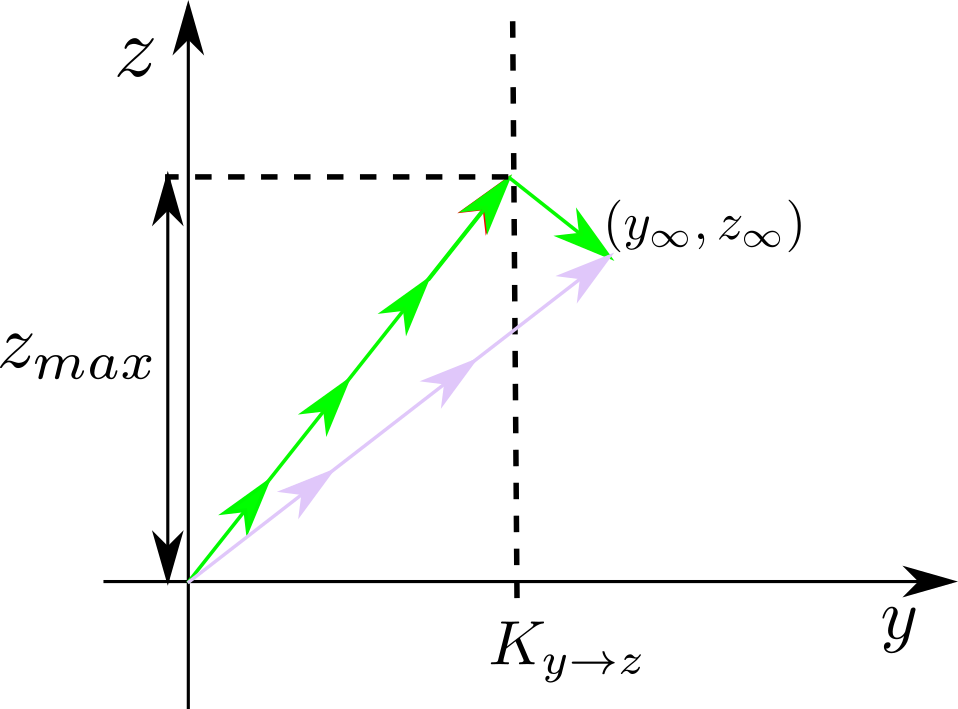
\includegraphics[width=2.8in]
{autoregulons/i1-ffl-speedup.png}
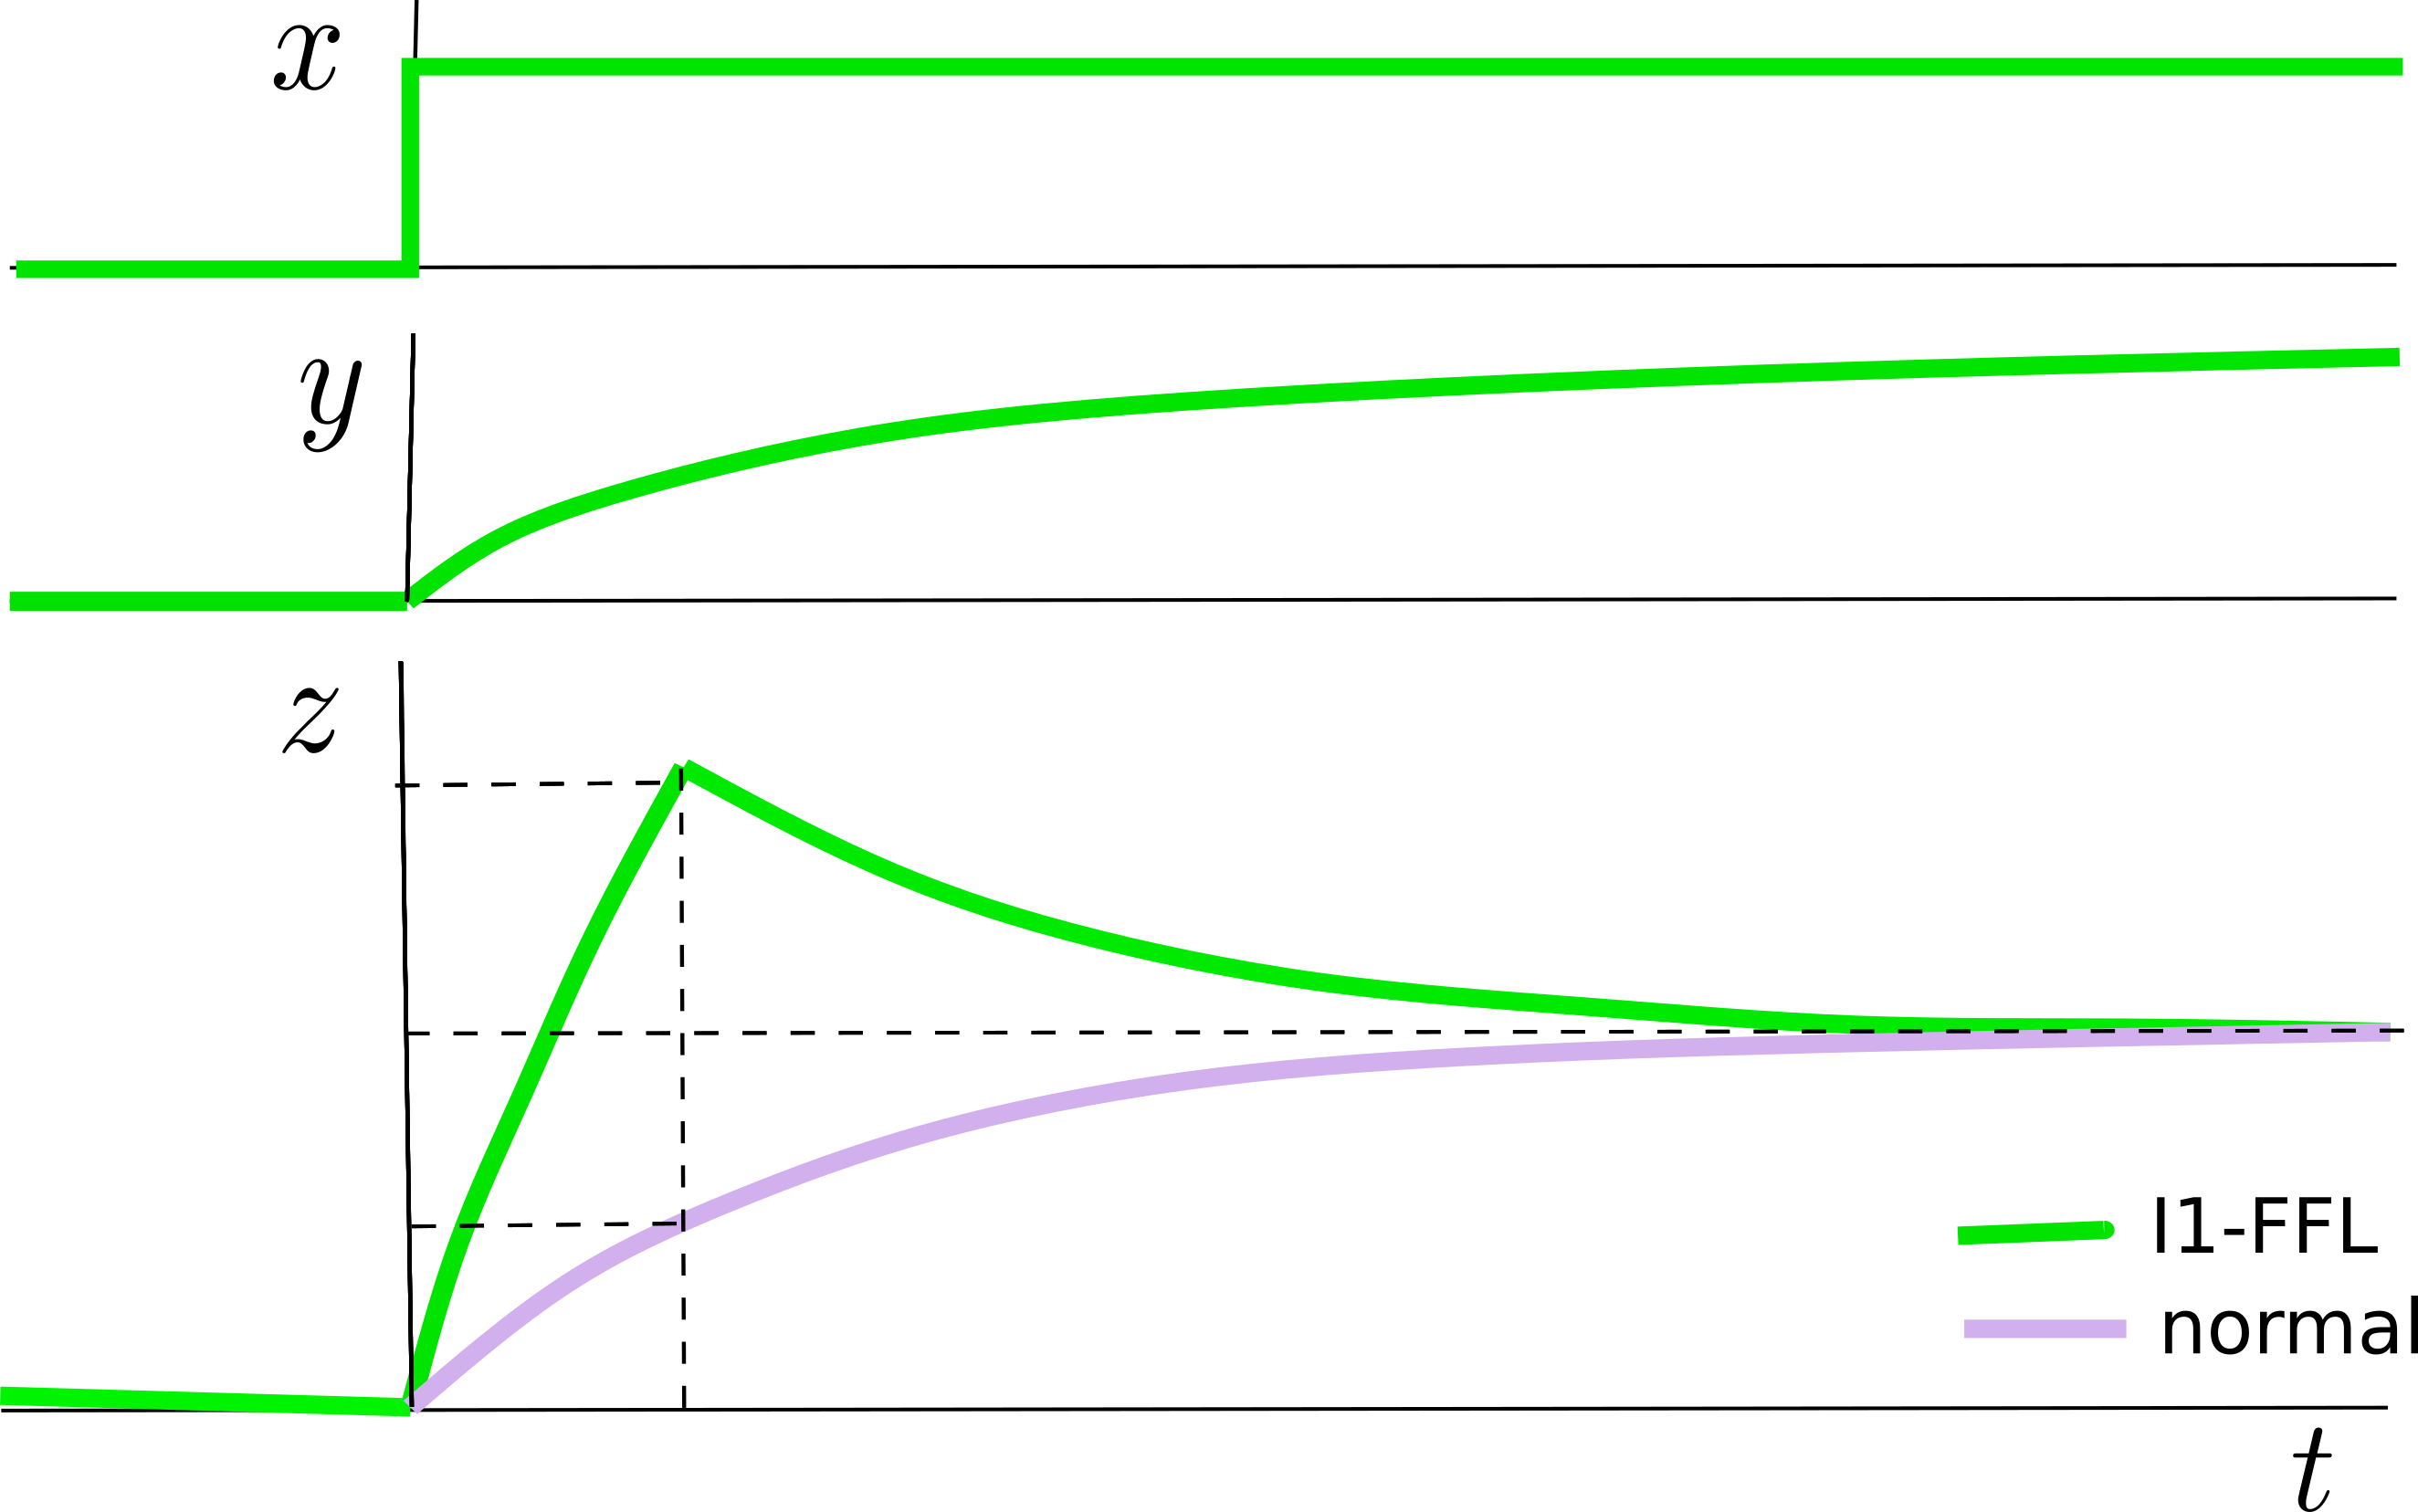
\includegraphics[width=2.8in]
{autoregulons/i1-ffl-green.png}
\caption{For I1-FFL, $x(t), y(t), z(t)$
assuming $x(t)$ step function rising 
from 0 at $t=0$.}
\label{fig-i1-ffl}
\end{figure}

See Fig.\ref{fig-i1-ffl}
for a pictorial
representation of what we will prove in this section.

We will assume $z<K_3$ always so $\indi(z<K_3)=1$.

\beq
x=\xi \indi(x>0)
\eeq
If $x>\max(K_{x\rarrow y}, K_{x\rarrow z})$,


\beq
\left\{
\begin{array}{l}
\dot{y}=-\alp_2 y + \beta_2 
\\
\dot{z}=-\alp_3 z + \beta_3 +
\beta_{12} \indi(y<K_{y\rarrow z})
\end{array}
\right.
\eeq
Let 

\beq
y_\infty = \frac{\beta_2}{\alp_2}\;,\quad
z_\infty = \frac{\beta_3}{\alp_3}\;\quad
z_\infty' = \frac{\beta_3+\beta_{12}}{\alp_3}
\eeq

If $y(0)=0$, then (see Fig.\ref{fig-i1-ffl})

\beq
y = y_\infty(1-e^{-\alp_2 t})
\eeq
and

\beq
z=\left\{
\begin{array}{ll}
z_\infty'(1- e^{-\alp_3 t})
& \text{ for } y<K_{y\rarrow z}
\\
z_{max} e^{-\alp_3 (t-t_{max})}+ z_\infty(1- e^{-\alp_3 (t-t_{max})})
& \text{ for } y>K_{y\rarrow z}
\end{array}
\right.
\eeq
where 

\beq
K_{y\rarrow z}=y_\infty(1- e^{-\alp_2 t_{max}})
\eeq

\beq
z(t_{max})=z_{max}= z_\infty'
(1-e^{-\alp_3 t_{max}})
\eeq

\subsection{Chain of autoregulons}

chains (cascades) of autoregulons
connected by highpass and lowpass filters

\beq\begin{array}{ccc}
(a)&
\xymatrix@C =3.5pc{
\Rect{\rvx^\redominus}\ar[r]|\redoplus
&\Rect{\rvy}\ar[r]|\redoplus
&\Rect{\rvz}
}
&
\left\{
\begin{array}{l}
\dot{x}= -\alp_x x +\beta_x\indi(x<K_x)
\\
\dot{y}= -\alp_y y + \beta_{x\rarrow y}
\indi(K_{x\rarrow y}>x)
\\
\dot{z}= -\alp_z z + \beta_{y\rarrow z}
\indi(K_{y\rarrow z}>y)
\end{array}
\right.
\\
\\
(b)&
\xymatrix@C=3.5pc{
\Rect{\rvx^\redominus}\ar[r]|\redominus
&\Rect{\rvy}\ar[r]|\redominus
&\Rect{\rvz}
}
&\left\{
\begin{array}{l}
\dot{x}= -\alp_x x +\beta_x\indi(x<K_x)
\\
\dot{y}= -\alp_y y + \beta_{x\rarrow y}
\indi(K_{x\rarrow y}<x)
\\
\dot{z}= -\alp_z z + \beta_{y\rarrow z}
\indi(K_{y\rarrow z}<y)
\end{array}
\right.
\end{array}
\eeq

\begin{figure}[h!]
\centering
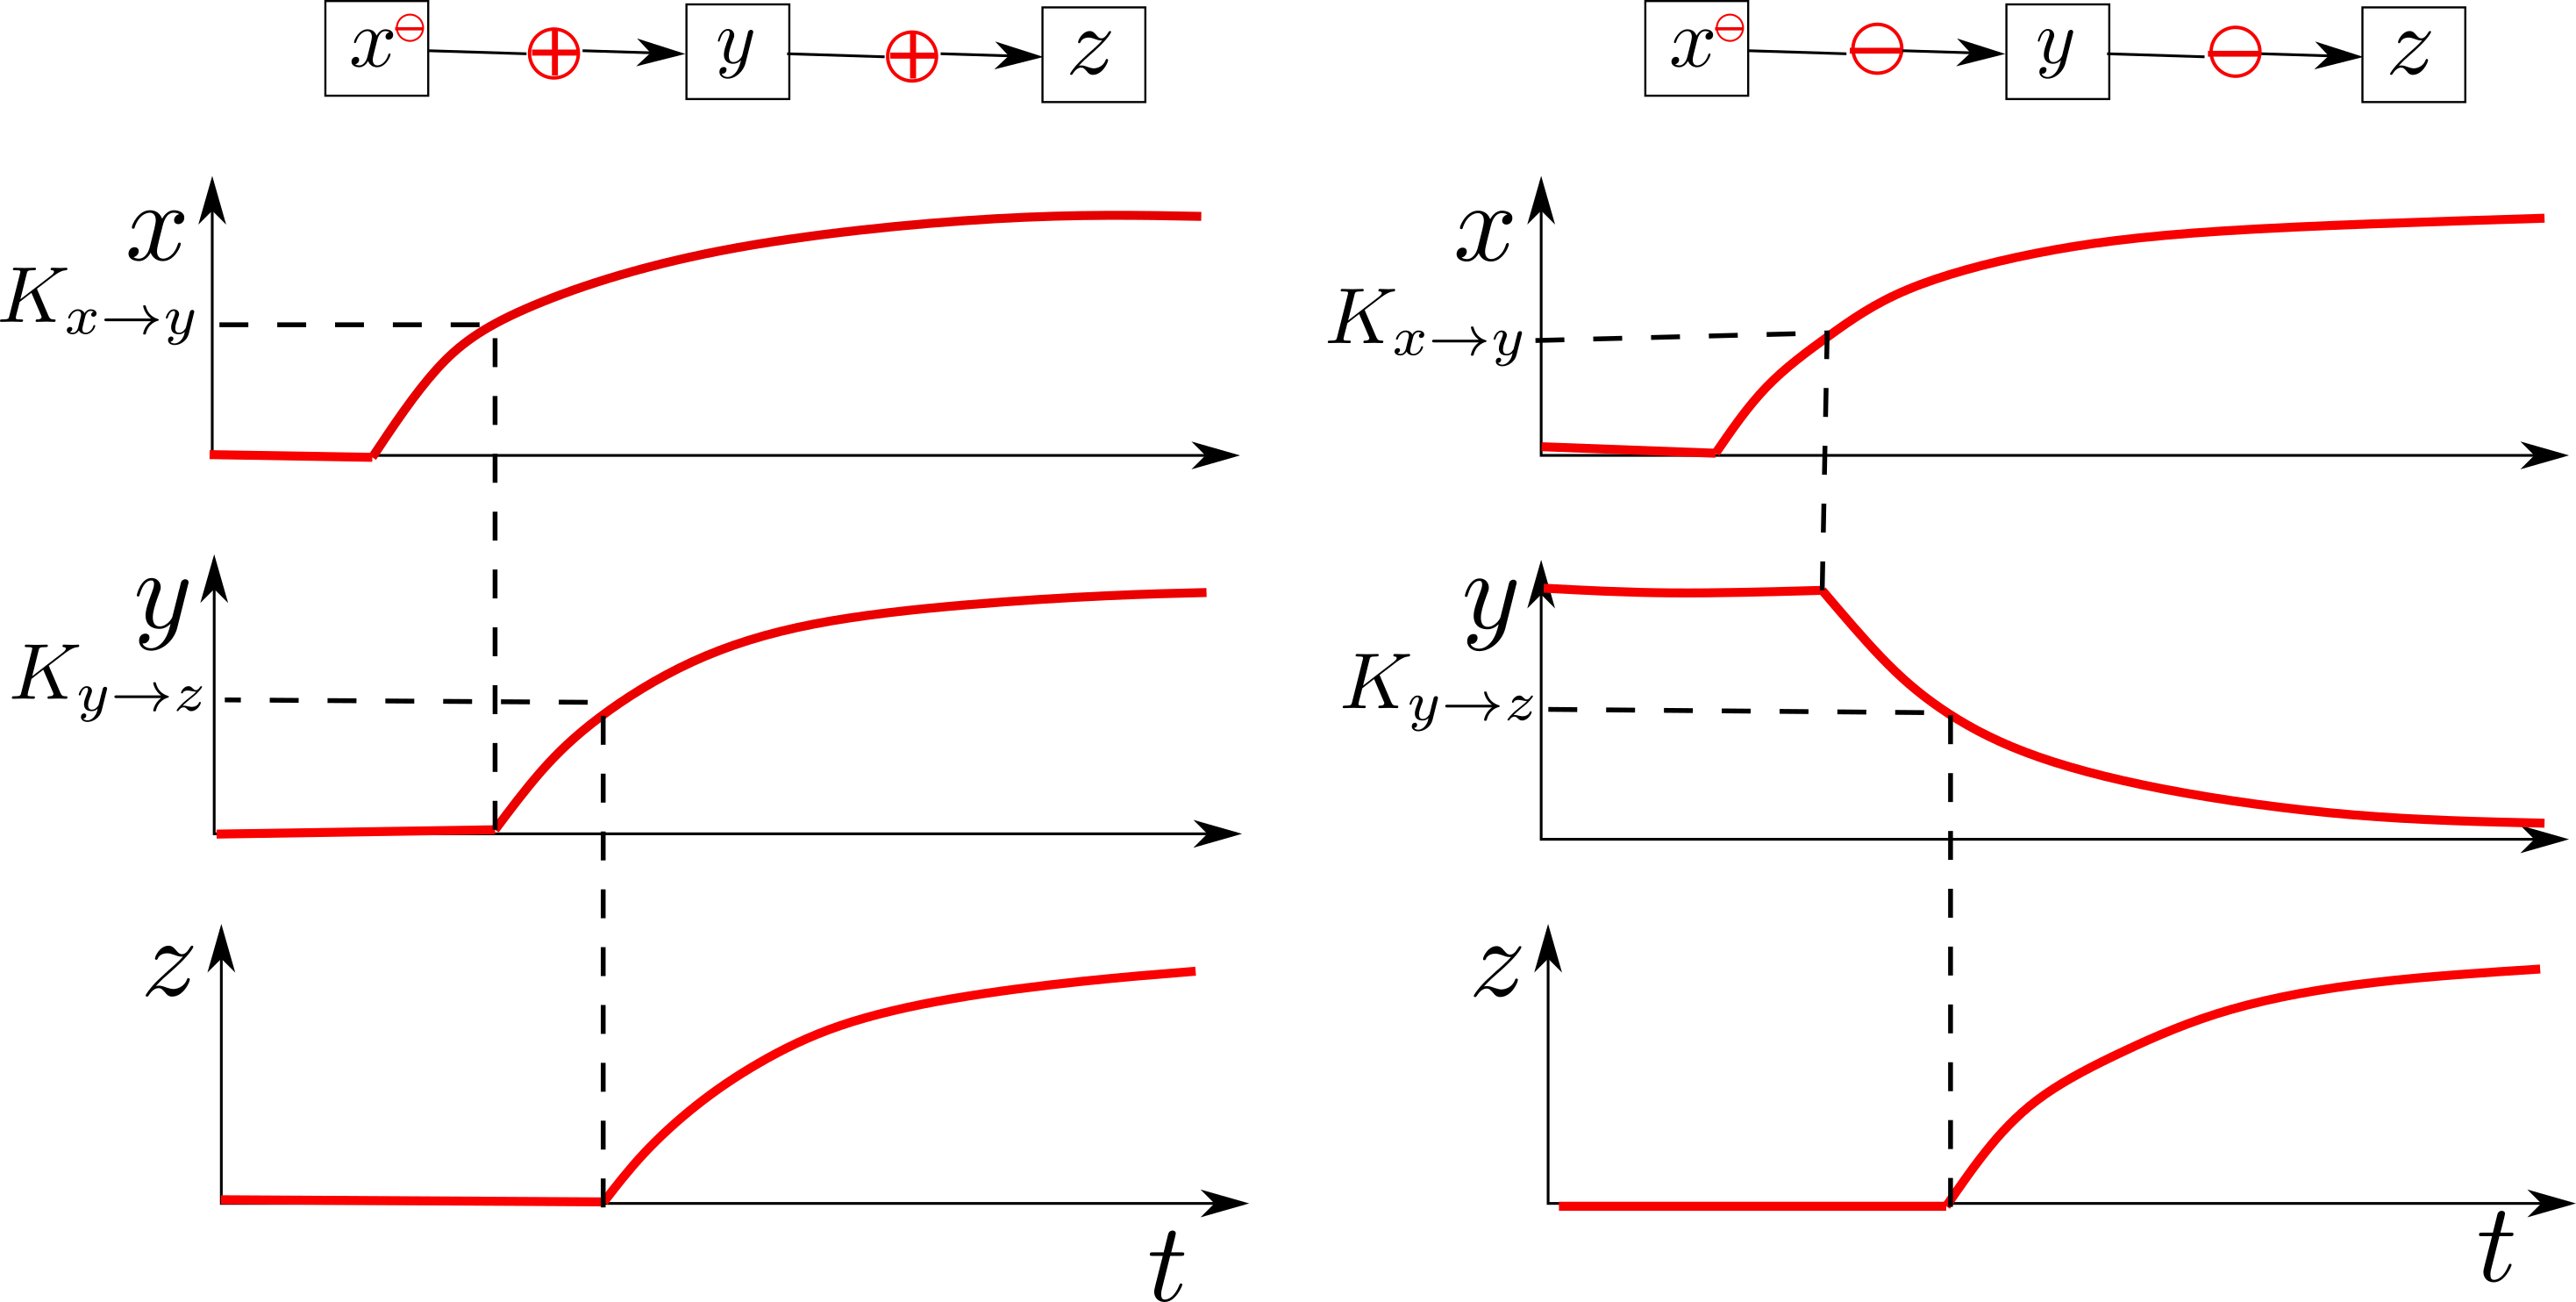
\includegraphics[width=4.7in]
{autoregulons/autoreg-cascade.png}
\caption{Chain of 3 autoregulons. 
 }
\label{fig-autoreg-cascade}
\end{figure}

\begin{enumerate}[(a)]
\item {\bf highpass filter chain}

Let 

\beq
x_\infty = \frac{\beta_x}{\alp_x}\;,\;\;
y_\infty = \frac{\beta_{x\rarrow y}}{\alp_y}\;,\;\;
z_\infty = \frac{\beta_{y\rarrow z}}{\alp_y}
\eeq
 
If $x(0)=0$, then
\beq
x=
x_\infty(1-e^{-\alp_x t})
\quad\text{for $t>0$}
\eeq
If $y=0$ for $t<t_{lag, y}$, then

\beq
y = y_\infty(1 - e^{-\alp_y(t-t_{lag, y})})
\quad\text{for $t>t_{lag, y}$}
\eeq
where $x(t_{lag, y})= K_{x\rarrow y}$.

If $z=0$ for $t<t_{lag, z}$, then

\beq
z = z_\infty(1 - e^{-\alp_z(t-t_{lag, z})})
\quad\text{for $t>t_{lag, z}$}
\eeq
where $y(t_{lag, z})= K_{y\rarrow z}$.

\item {\bf lowpass filter chain}

Let 

\beq
x_\infty = \frac{\beta_x}{\alp_x}\;,\;\;
y_\infty = \frac{\beta_{x\rarrow y}}{\alp_y}\;,\;\;
z_\infty = \frac{\beta_{y\rarrow z}}{\alp_y}
\eeq
 
If $x(0)=0$, then
\beq
x=
x_\infty(1-e^{-\alp_x t})
\quad\text{for $t>0$}
\eeq
If $y=y_0$ for $t<t_{lag, y}$, then

\beq
y = y_0 e^{-\alp_y(t-t_{lag, y})}
\quad\text{for $t>t_{lag, y}$}
\eeq
where $x(t_{lag, y})= K_{x\rarrow y}$.

If $z=0$ for $t<t_{lag, z}$, then

\beq
z = z_\infty(1 - e^{-\alp_z(t-t_{lag, z})})
\quad\text{for $t>t_{lag, z}$}
\eeq
where $y(t_{lag, z})= K_{y\rarrow z}$.
\end{enumerate}


\subsection{Repressilator}
See Ref.\cite{liepe2013maximizing}

Repressilator net

\beq
\xymatrix{
&\ar[dr]&\rvm_1\ar[dr]|\redplus
\ar[d]|\redminus
&\rvp_1\ar[d]|\redminus
\ar@/_1pc/[dddlll]|\redominus
\\
\ar@/_1pc/[dd]
&
&\dot{\rvm_1}
&\dot{\rvp_1}
&\ar@/_1pc/[dd]
\\
\rvm_2\ar[dr]|\redplus
\ar[d]|\redminus
&\rvp_2\ar[d]|\redminus
\ar[drrr]|\redominus
&&&\rvm_3\ar[dr]|\redplus
\ar[d]|\redminus
&\rvp_3\ar[d]|\redminus
\ar[lllu]|\redominus
\\
\dot{\rvm_2}&\dot{\rvp_2}
&&&\dot{\rvm_3}&\dot{\rvp_3}
}
\left\{
\begin{array}{l}
\dot{m_1} = -m_1 + \frac{\alp}{1+p_3^n}+\alp_0
\\
\dot{m_2} = -m_2 + \frac{\alp}{1+p_1^n}+\alp_0
\\
\dot{m_3} = -m_3 + \frac{\alp}{1+p_2^n}+\alp_0
\\
\dot{p_i} = \beta(m_i-p_i)\quad \text{ for } i=1,2,3
\end{array}
\right.
\label{eq-repress-bnet}
\eeq
\begin{figure}[h!]
\centering
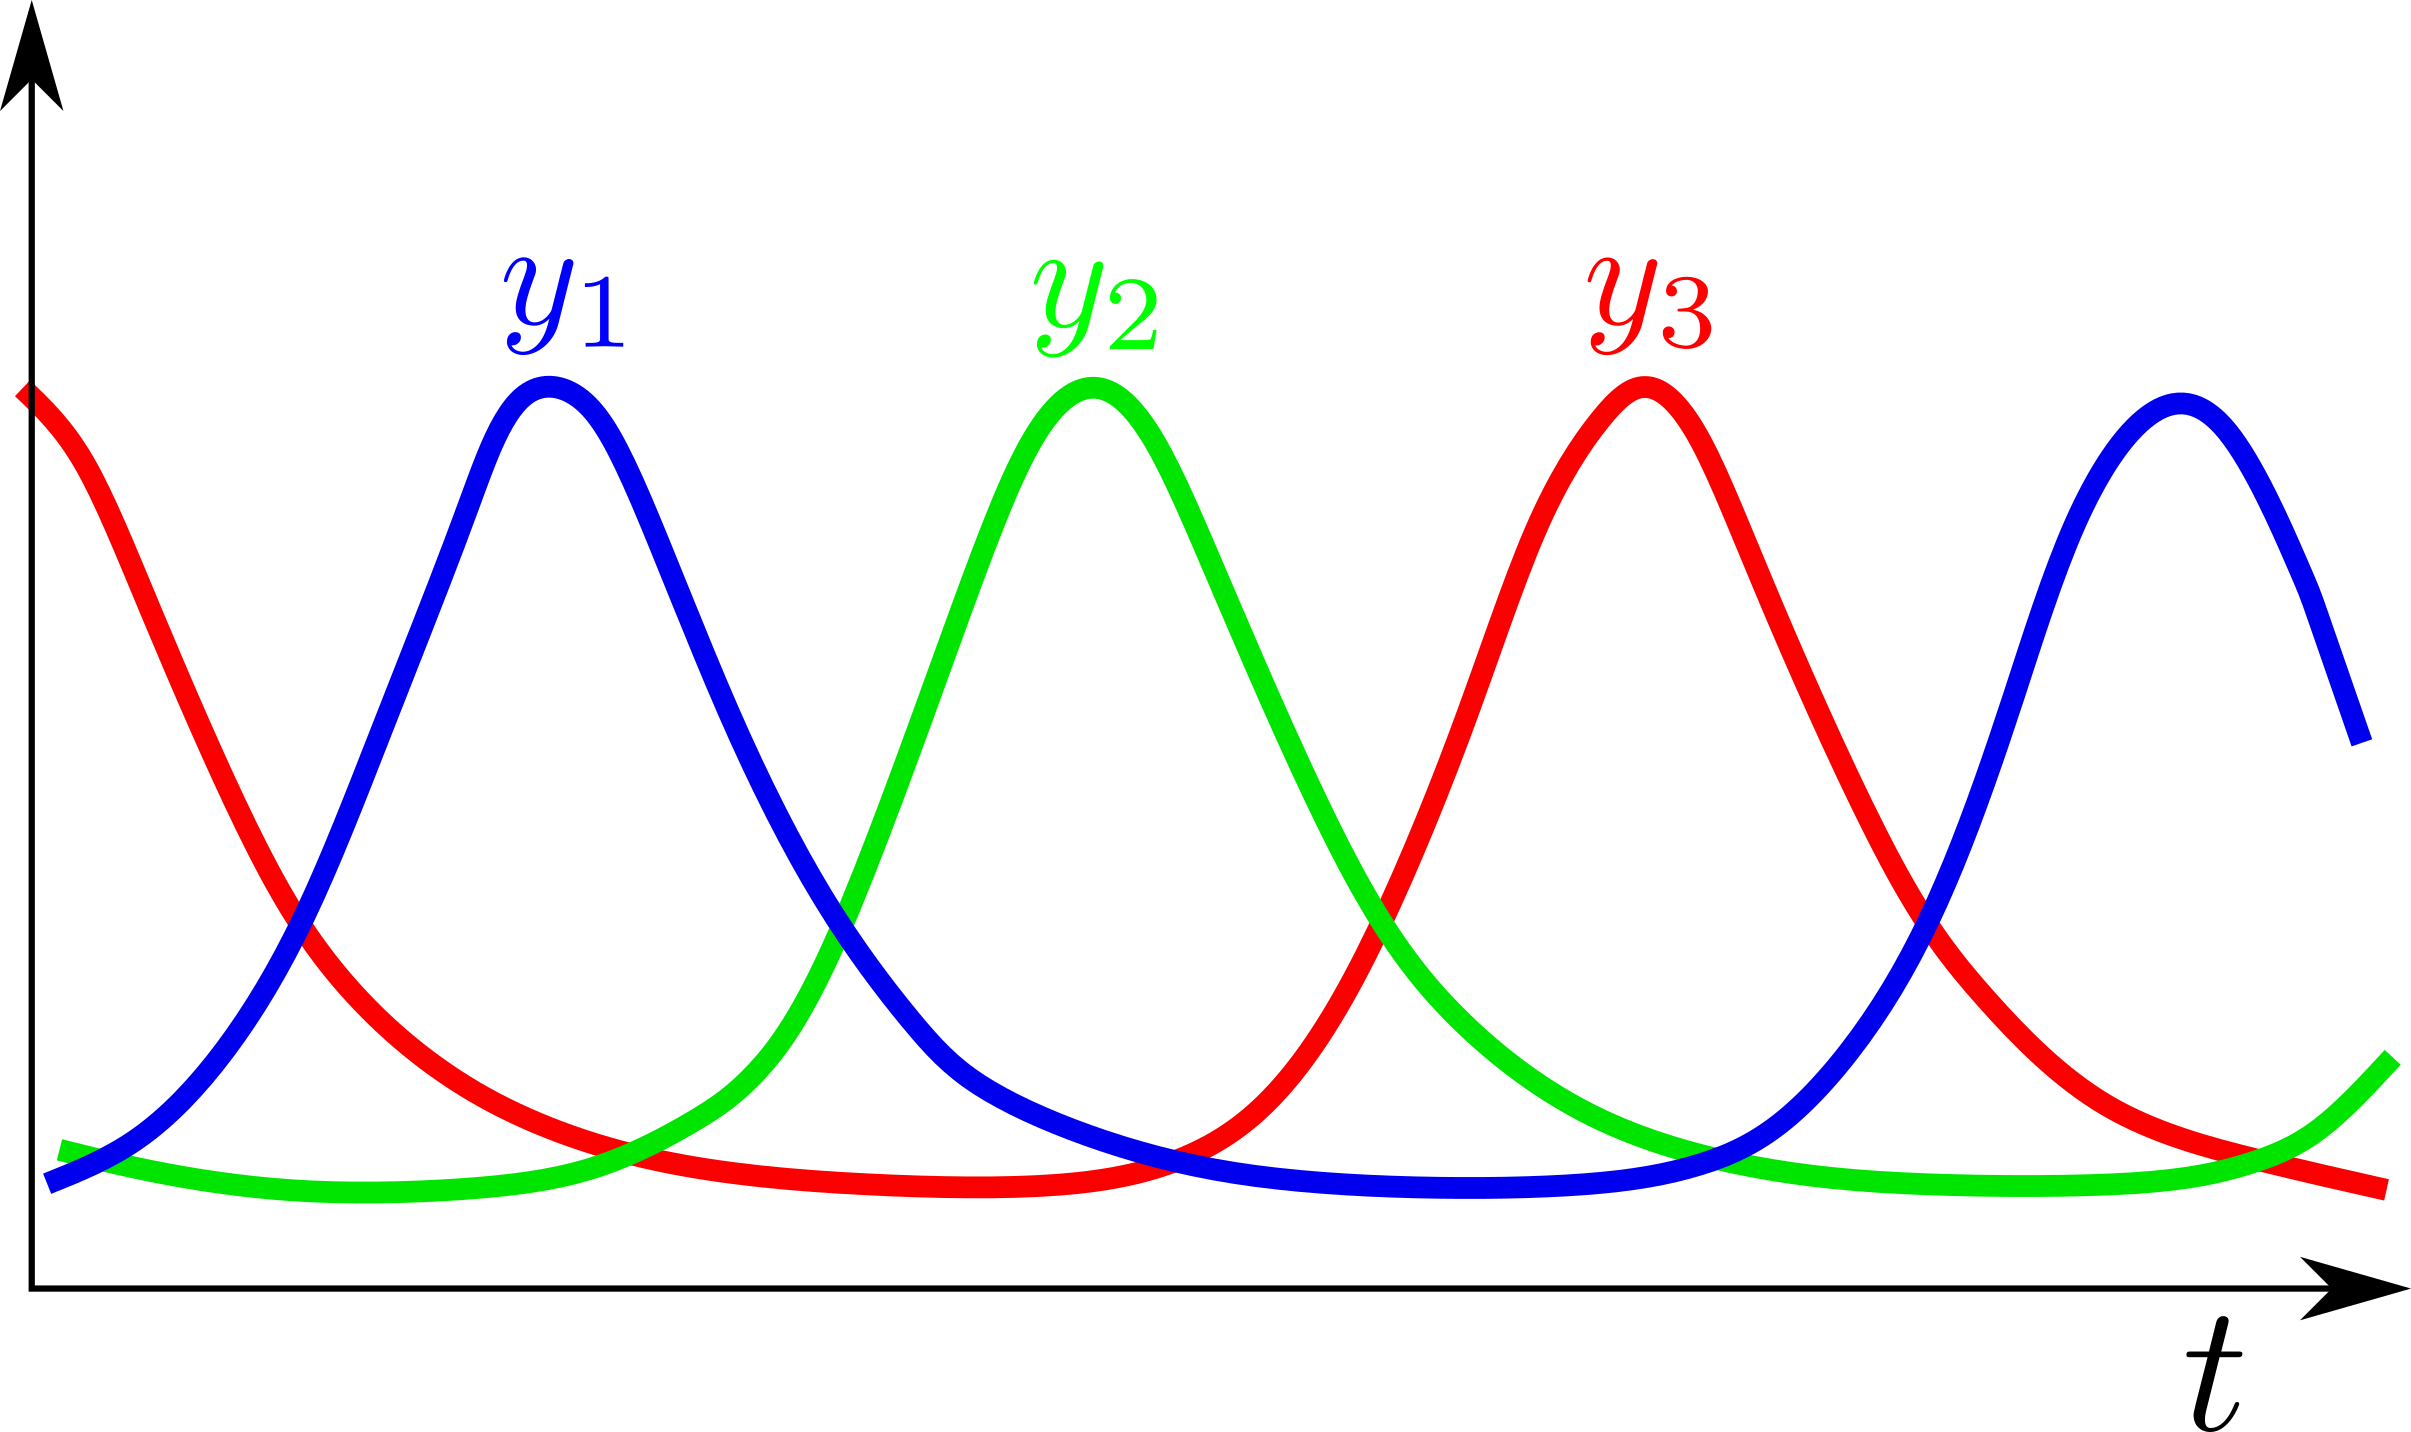
\includegraphics[width=2.5in]
{autoregulons/interlaced-3.png}
\caption{The repressilator net
produces 3 interlaced peak trains  $y_1(t), y_2(t), y_3(t)$, where $y_i=m_i -1$. 
 }
\label{fig-interlaced-3}
\end{figure}



\beq
\Gamma=
\left[
\begin{array}{ccc}
0&0&1
\\
1&0&0
\\
0&1&0
\end{array}
\right]
\eeq
$\Gamma$ is permutation matrix so

\beq
\Gamma^2=1 
\eeq
Note this implies
\beq
0=1-\Gamma^2 =(1+\Gamma)(1-\Gamma)
\eeq
Define the projection operators

\beq
\pi_\pm = \frac{1\pm\Gamma}{2}
\eeq
It is easy to check that
\beq
\left\{
\begin{array}{l}
\pi_+\pi_-=\pi_-\pi_+ =0
\\
\pi_-^2=\pi_-\;,\;\;\pi_+^2=\pi_+
\\
\pi_+ +\pi_-=1
\end{array}
\right.
\eeq

\beq
\vec{u}= [1,1,1]^T
\eeq

\beq
\pi_- \vec{u}=0\;,\;\;\pi_+ \vec{u}=\vec{u}
\eeq


Let 

\beqa
\frac{\alp}{1+p_i^n}
&\approx& \frac{\alp}{2}(1-\frac{n}{2}
(p_i-1))
\\
&=&-\gamma (p_i-1) + \frac{\alp}{2}
\eeqa

\beq
\vec{x}=\vec{p}-1
\;,\;\;
\vec{y} = \vec{m}-1
\eeq

\beq
\left\{
\begin{array}{l}
\dot{\vec{y}} = -\vec{y}
-\gamma \Gamma\vec{x} + c\vec{u}
\\
\dot{\vec x} = \beta(\vec{y}-\vec{x})
\end{array}
\right.
\eeq

\beq 
\call_1 = \partial_t + 1
\;,\;\;
\call_\beta = \partial_t +\beta
\eeq

\beq
\left\{
\begin{array}{l}
\call_1\vec{y} =
-\gamma \Gamma\vec{x} + c\vec{u}
\\
\call_\beta \vec x = \beta\vec{y}
\end{array}
\right.
\eeq

\beq
\vec{x} = 
\beta\call_\beta^{-1}\vec{y}
\eeq

\beq
\call_1\vec{y}=
-\gamma\beta \Gamma\call_\beta^{-1}\vec{y}
+c\vec{u}
\eeq

\beq
\call_\beta\call_1\vec{y}=
-\gamma\beta \underbrace{\Gamma}_{2\pi_+ -1}\vec{y}
+\beta c\vec{u}
\eeq

\beq
\vec{y}_\pm =\pi_\pm \vec{y}\;,\;\; 
\eeq


\beq
\left\{
\begin{array}{l}
(\call_\beta\call_1+2\gamma\beta) \vec{y}_+ = \beta c\vec{u}
\\
(\call_\beta\call_1 -\gamma\beta)\vec{y}_-=0
\end{array}
\right.
\eeq

\beq
\call_\beta\call_1 =
\partial_t^2 + (1+\beta)\partial_t + \beta
\eeq
One can solve for $\vec{y}_+$
and $\vec{y}_-$ separately.
Each component of $\vec{y}_+$
obeys a forced damped harmonic oscillator
ODE with natural frequency $\sqrt{(1+2\gamma)\beta}$. 
Each component of $\vec{y}_-$
obeys a forced damped harmonic oscillator
ODE with natural frequency  $\sqrt{(1-\gamma)\beta}$.


%\beq
%\xymatrix{
%&\ar[dr]&\rvm_1\ar[dr]|\redplus
%\ar[d]|\redminus
%&\rvp_1\ar[d]|\redminus
%\ar@/_1pc/[dddlll]|\redominus
%\\
%\ar@/_1pc/[dd]
%&
%&\dot{\rvm_1}
%&\dot{\rvp_1}
%&\ar@/_1pc/[dd]
%\\
%\rvm_2\ar[dr]|\redplus
%\ar[d]|\redminus
%&\rvp_2\ar[d]|\redminus
%\ar[drrr]|\redominus
%&&&\rvm_3\ar[dr]|\redplus
%\ar[d]|\redminus
%&\rvp_3\ar[d]|\redminus
%\ar[lllu]|\redominus
%\\
%\dot{\rvm_2}&\dot{\rvp_2}
%&&&\dot{\rvm_3}&\dot{\rvp_3}
%}
%\left\{
%\begin{array}{l}
%\dot{m_1} = -m_1 + \frac{\alp}{1+p_3^n}+\alp_0
%\\
%\dot{m_2} = -m_2 + \frac{\alp}{1+p_1^n}+\alp_0
%\\
%\dot{m_3} = -m_3 + \frac{\alp}{1+p_2^n}+\alp_0
%\\
%\dot{p_i} = \beta(m_i-p_i)\quad \text{ for } i=1,2,3
%\end{array}
%\right.
%\label{eq-repress-bnet}
%\eeq
%For 
% all $i$, 
% assume $\dot{p}_i\approx 0$.
%Hence $p_i\approx m_i$.
%Assume also that $x_i=
%m_i-1\approx 0$.
%Then Eq.(\ref{eq-repress-bnet}) reduces to
%
%\beq
%\left\{
%\begin{array}{l}
%\dot{x}_1=
%-x_1
%+\frac{\alp}{2}(
%1-\frac{n}{2}x_3)
%+\alp_0 - 1
%\\
%\dot{x}_2=
%-x_2
%+\frac{\alp}{2}(
%1-\frac{n}{2}x_1)
%+\alp_0 -1
%\\
%\dot{x}_3=
%-x_3
%+\frac{\alp}{2}(
%1-\frac{n}{2}x_2)
%+\alp_0 -1
%\end{array}
%\right.
%\eeq
%Next let 
%$\gamma = \frac{\alp n}{4}$ and 
%$c=\alp_0 -1 + \frac{\alp}{2}$
%to get
%
%\beq
%\left\{
%\begin{array}{l}
%\dot{x}_1=
%-x_1
%-\gamma x_3
%+c
%\\
%\dot{x}_2=
%-x_2
%-\gamma x_1
%+c
%\\
%\dot{x}_3=
%-x_3
%-\gamma x_2
%+c
%\end{array}
%\right.
%\eeq
%Finally, let $y_i = x_i-M$
%for all $i$,
%where $M=\frac{-c}{1+\gamma}$ to get
%
%\beq
%\left\{
%\begin{array}{l}
%\dot{y}_1=
%-y_1
%-\gamma y_3
%\\
%\dot{y}_2=
%-y_2
%-\gamma y_1
%\\
%\dot{y}_3=
%-y_3
%-\gamma y_2
%\end{array}
%\right.
%\eeq
%
%\beq
%\dot{\vec{y}}=-A \vec{y}
%\eeq
%with $\vec{y}=(y_1, y_2, y_3)^T$
%and
%
%\beq
%A=
%\left[
%\begin{array}{ccc}
%\alp_1 & 0&\gamma_1
%\\
%\gamma_2&\alp_2&0
%\\
%0&-\gamma_3&\alp_3
%\end{array}
%\right]
%\eeq
%
%\beq
%y = y_0 e^{-\lam t}
%\implies (A-\lam)y=0
%\eeq
%
%\beq
%\det (A -\lam) = (\alp_1-\lam)(\alp_2-\lam)
%(\alp_3 -\lam) - \gamma_1 \gamma_2 \gamma_3
%\eeq
%For $\alp_1=\alp_2=\alp_3=0$,
%get 
%
%\beqa
%\lam &=& (-\gamma_1\gamma_2\gamma_3)^{\frac{1}{3}}
%\\
%&=&
%(\gamma_1\gamma_2\gamma_3)^{\frac{1}{3}}
%e^{i\frac{1}{3}(-\pi + 2\pi n)}
%\label{eq-3-complex-solutions}
%\eeqa
%for $n=0,1,2$.
%If the $\alp_i$ are very small,
%then we approximate
%
%\beq
%\lam^3 -\underbrace{(\alp_1 +\alp_2+\alp_3)}_\tau \lam^2
%=-\gamma_1\gamma_2\gamma_3
%\eeq
%Let $\lam_c$ be one of the
%3 complex solutions given
%by Eq.(\ref{eq-3-complex-solutions}).
%Let $\tau = \tr A$. Then to first order in $\tau$,
%
%\beq
%\lam = \lam_c + \frac{\tau}{3}
%\eeq



\subsection{SIM net}
Single Input Module (SIM) net

SIM net

\beq
\xymatrix@R=4pc{
&\Rect{\rvx^\redominus}
\ar[dl]|\redoplus_{K_1}
\ar[d]|\redoplus_{K_2}
\ar[dr]|\redoplus^{K_3}
\\
\Rect{\rvy_1}
&\Rect{\rvy_2}
&\Rect{\rvy_3}
}
\left\{
\begin{array}{ll}
\dot{x} =-\alp x + \beta\theta(x<K)\indi_{0}^{t_2}(t)
\\
\dot {y_i} = -\alp_i y_i + \beta_i\indi(x>K_i)
& \text{for $i=1,2,3$}
\end{array}
\right.
\eeq

\begin{figure}[h!]
\centering
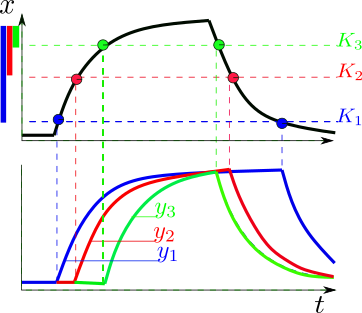
\includegraphics[width=2.8in]
{autoregulons/sim-net.png}
\caption{For SIM net, response  $y_1(t), y_2(t), y_3(t)$ to stimulus $x(t)$.
Blue is first and last out. FILO. In other words, SIM produces pulses
such that pulse-rise-edges and pulse-drop-edges are in
reverse  order.}
\label{fig-sim-net}
\end{figure}

Let 

\beq
x_\infty = \frac{\beta}{\alp}
\;,\;\;
y_{\infty,i} = \frac{\beta_i}{\alp_i}\quad
\text{for $i=1,2,3$}
\eeq
If $x(0)=0$ and $x(t_2)<K$

\beq
x=
\left\{
\begin{array}{ll}
x_\infty(1-e^{-\alp t})& \text{if $t<t_2$}
\\
x_{max}e^{-\alp t}
& \text{if $t>t_2$}
\end{array}
\right.
\eeq
Assume $K_1, K_2, K_3< x_\infty
$. Then

\beq
y_i=
\left\{
\begin{array}{ll}
y_{\infty, i}(1-e^{-\alp_i (t-t_{lag,i})})
&\text{if$x>K_i$}
\\
y_{max,i}e^{-\alp_i(t-t_{max,i})}
&\text{if $x<K_i$ }
\end{array}
\right.
\eeq





\subsection{Flagellum net}

\beq
\xymatrix@C=3pc{
&\Rect{\rvx^\redominus}
\ar[d]|\redoplus
\ar[dl]|\redoplus_{K_1}
\ar[dr]|\redoplus^{K_2}
\\
\bigotimes\ar[d]
&\Rect{\rvy}\ar[l]|\redoplus^{K'_1}
\ar[r]|\redoplus_{K'_2}
&\bigotimes\ar[d]
\\
\Rect{\rvz_1}&
&\Rect{\rvz_2}
}
\left\{
\begin{array}{l}
\dot{x}= -\alp_x x + \beta_x (x<K_x)\indi_{0}^{t_2}(t)
\\
\dot {y} = -\alp_y y + \beta_y\indi (x>K_y)
\\
\dot{z}_1= -\alp_1 x + \beta_1\indi(x>K_1)\indi(y>K_1')
\\
\dot{z}_2= -\alp_2 y + \beta_2\indi(x>K_2)\indi(y>K_2')
\end{array}
\right.
\eeq

\begin{figure}[h!]
\centering
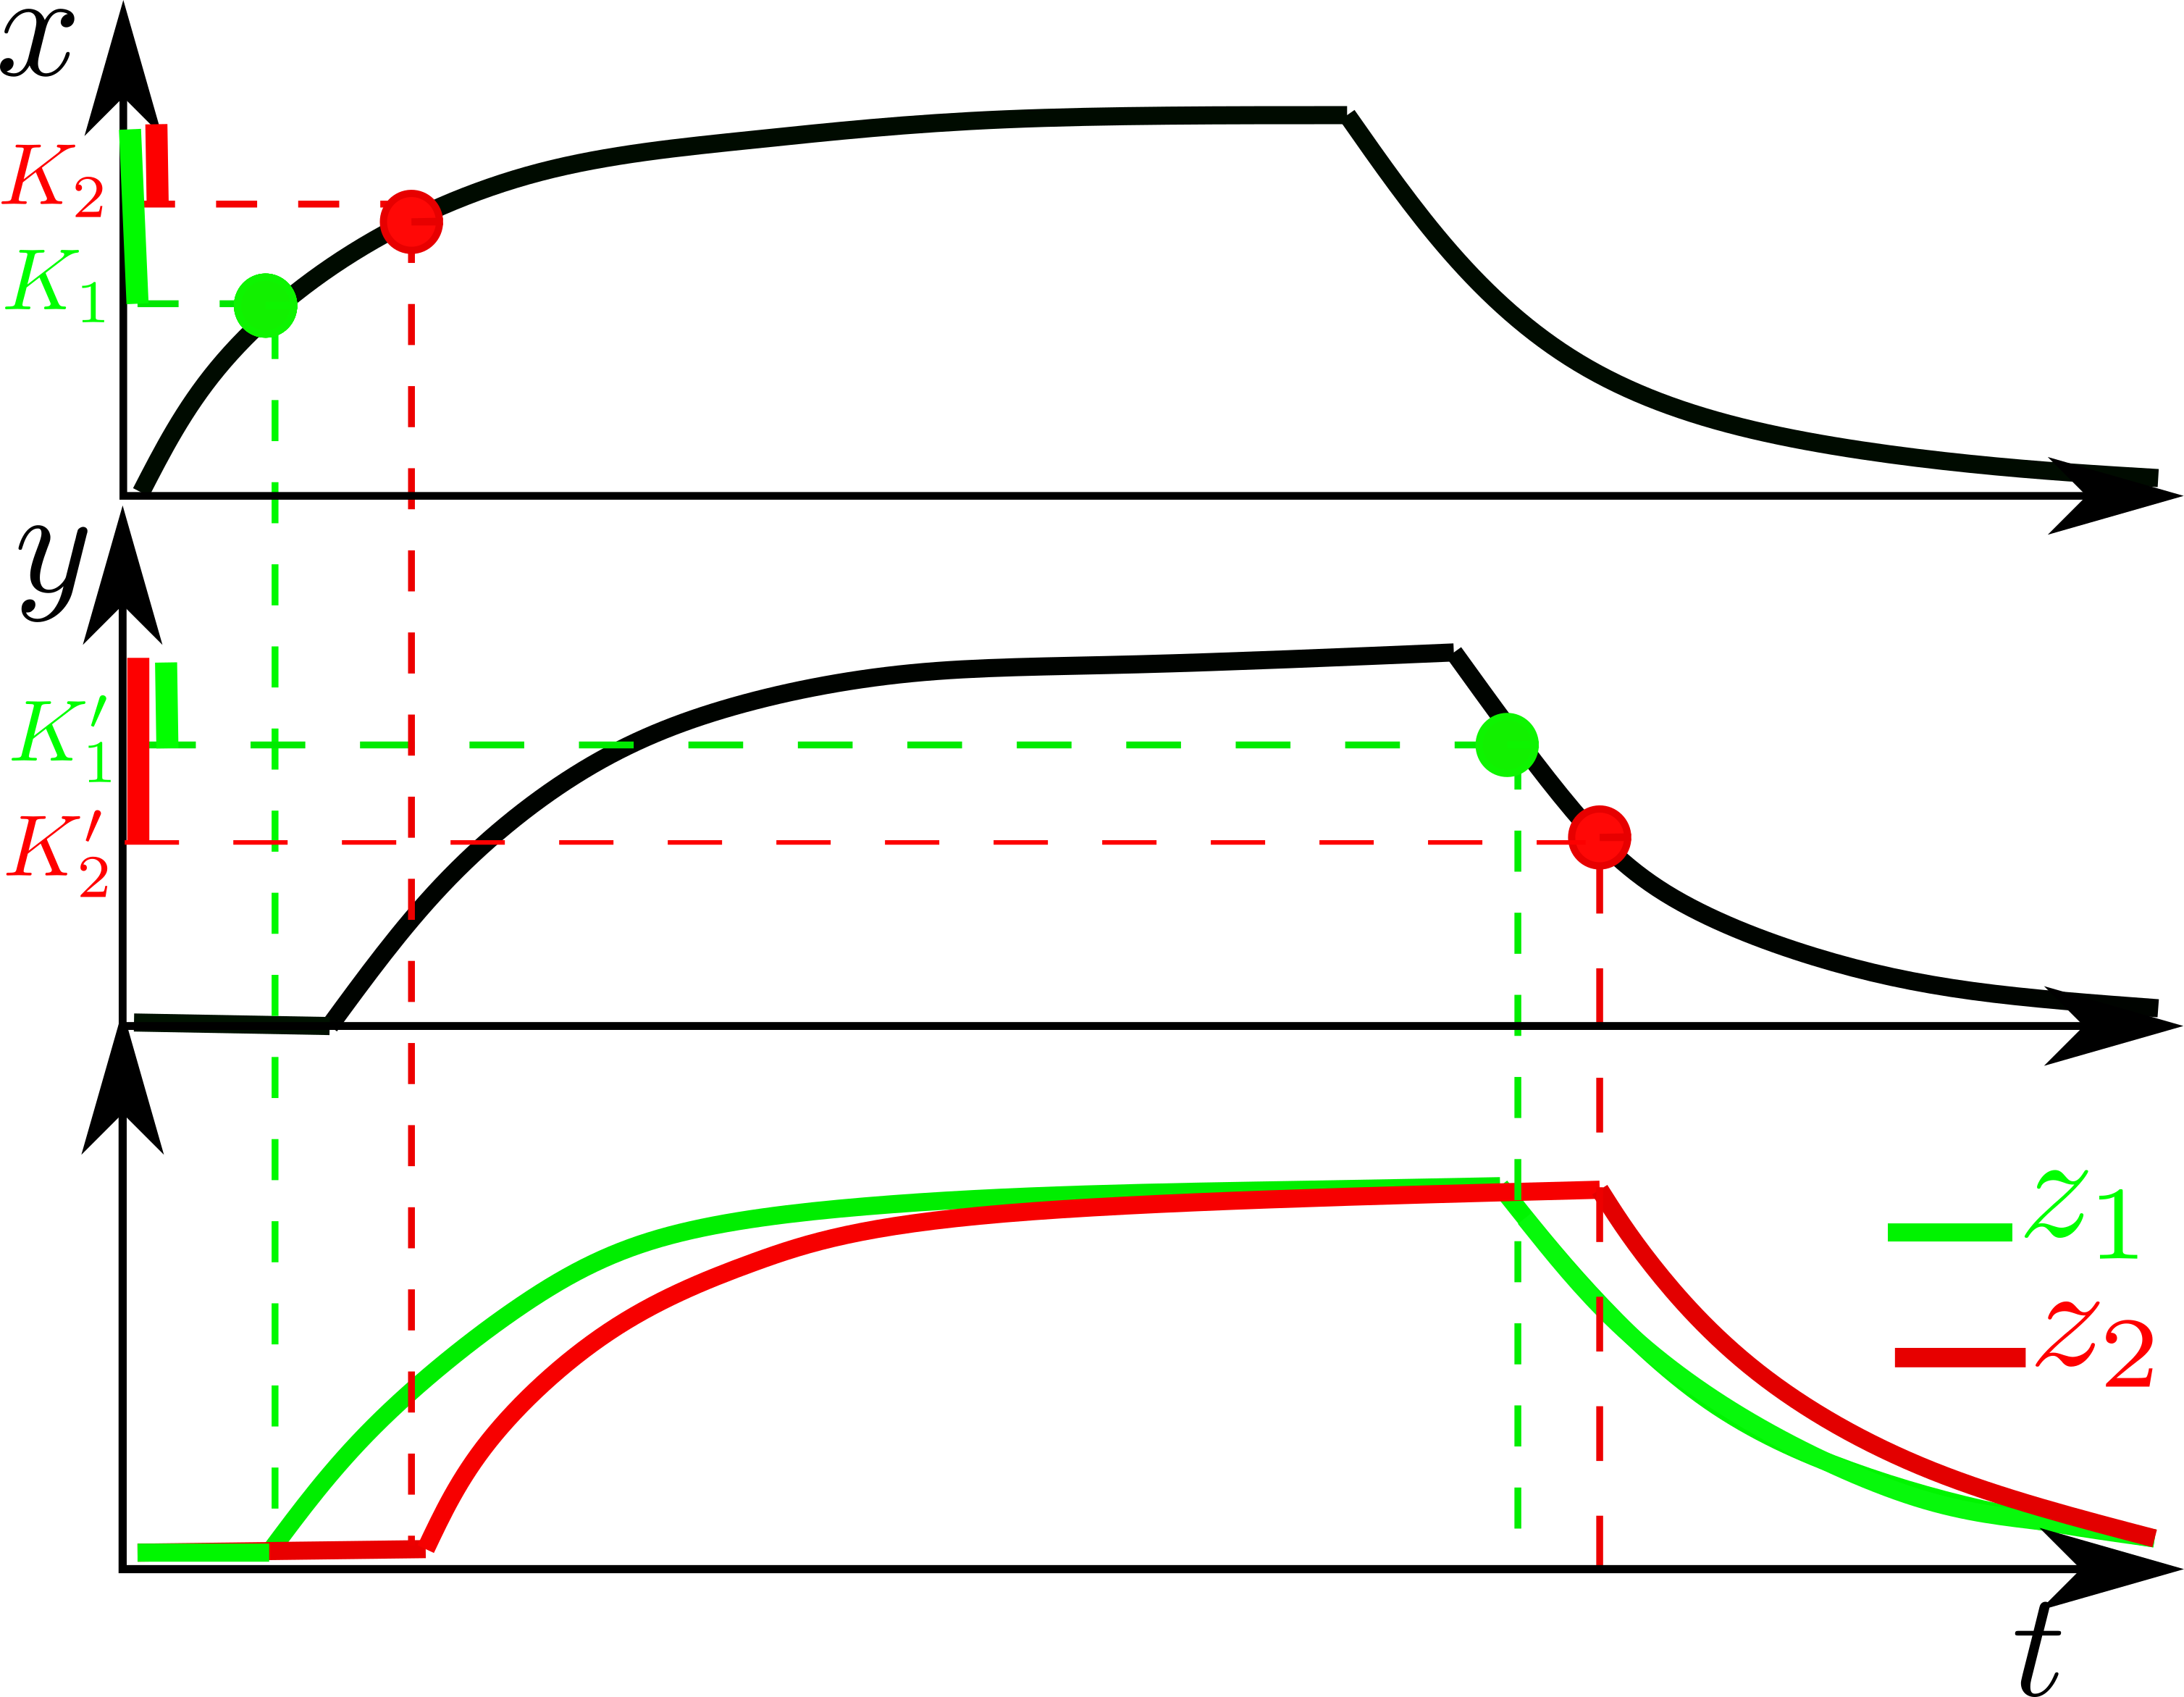
\includegraphics[width=2.8in]
{autoregulons/flagellum.png}
\caption{For Flagellum net, response  $y(t), z_1(t), z_2(t)$ to stimulus $x(t)$. Green is first and first out. FIFO. In other words, the Flagellum net produces pulses
such that pulse-rise-edges and pulse-drop-edges are in
the same order.}
\label{fig-flagellum-net}
\end{figure}

Flagellum bnet. Assume $K_1<K_2$ and $K'_1 > K'_2$.

\beq
x_\infty= \frac{\beta_x}{\alp_x}\;,\;\;
y_\infty= \frac{\beta_x}{\alp_x}\;,\;\;
z_{\infty, 1}= \frac{\beta_x}{\alp_x}\;,\;\;
z_{\infty, 2}= \frac{\beta_x}{\alp_x}
\eeq

If $x(0)=0$

\beq
x=
\left\{
\begin{array}{ll}
x_\infty(1-e^{-\alp_x t})
&\text{if }t<t_2
\\
x_{max}e^{-\alp_x (t-t_{max})}
&\text{if }t>t_2
\end{array}
\right.
\eeq

If $y(t_{lag})=0$
\beq
y=
\left\{
\begin{array}{ll}
y_\infty(1-e^{-\alp_y (t-t_{lag})})
&\text{if }t_{lag}<t<t_2
\\
y_{max}e^{-\alp_y (t-t_{max})}
&\text{if }t>t_2
\end{array}
\right.
\eeq

For $i=1,2$, if $z(t_{lag, i})=0$
\beq
z_i=
\left\{
\begin{array}{ll}
z_{\infty, i}(1-e^{-\alp_i t_{lag, i}})
&\text{if }x>K_i
\\
z_{max, i}e^{-\alp_i (t-t_{max, i})} 
&
\text{if }y<K_i'
\end{array}
\right.
\eeq



\subsection{Bacillus Subtilis Sporation net}

\beq
\xymatrix{
&\Rect{\rvx_1}\ar[ddl]|\redplus
\ar[ddr]|\redplus
\\
&\Rect{\rvy_1}
\ar[dl]|\redminus
\ar[dr]|\redplus
\\
\bigotimes\ar[d]
&&\bigotimes\ar[d]
\\
\Rect{\rvz_1}
&&\Rect{\rvx_2}
\ar[d]|\redplus
\ar[ddl]|\redplus
\ar[ddr]|\redplus
\\
&&\Rect{\rvy_2}\ar[dl]|\redminus
\ar[dr]|\redplus
\\
&\bigotimes\ar[d]
&&\bigotimes\ar[d]
\\
&\Rect{\rvz_2}
&&\Rect{\rvz_3}
}
\eeq
Bacillus Subtilis  Sporation net


\subsection{Frog Egg Cell Cycle net}



Frog egg cell cycle net


\beq
h_\oplus (x)\approx \beta
\indi(x>K)\;,\;\;
h_\ominus (x)\approx \beta
\indi(x<K)
\eeq

\beqa
h_{\square}(x;K_1, K_2) &=&
h_\oplus(x; K_1)h_\ominus(x; K_2)
\\
&\approx & \beta'\indi_{K'_1}^{K'_2}(x)
\eeqa

\beq
\xymatrix{
X_0 \ar@<.8ex>[rr] 
&&X_p\ar@<.8ex>[ll]\ar@/_1pc/[l]\ar@/^1pc/@{-|}[l]
}
\eeq

\beq
\xymatrix{
\Rect{\rvx^{\color{red}\square}}
}=
\xymatrix{
\rvx
\ar@/_1pc/[d]_{-\square}
\ar@/^1pc/[d]^{\square}
\\
\dot{\rvx}
}
\quad
\left\{
\dot{x} = \underbrace{
-h_{\square}(x;K_1', K_2')
}_{\text{removal}} 
+ \underbrace{h_{\square}(x;K_1, K_2)}_{\text{production}}
\right.
\eeq

\beq
\xymatrix{
\Rect{\rvx^{\redoplus}}}
\quad
\left\{
\dot{x} = \underbrace{-\alp x}_{\text{removal}} 
+ \underbrace{h_\oplus(x)}_{\text{production}}
\right.
\eeq

\beq
\xymatrix@C=3pc{
\Rect{\rvx^{\color{red}\square}}
\fbackar{r}{\redoplus}{\redominus}
&\Rect{\rvy}
}
\quad
\left\{
\begin{array}{l}
\dot{x}=
-\gamma'_1\indi_{K_1'}^{K_2'}(x)
+\gamma_1\indi_{K_1}^{K_2}(x) +\beta_1\indi(y<K_{y\rarrow x})
\\
\dot{y}= -\alp_2 y +\beta_2\indi(x>K_{x\rarrow y})
\end{array}
\right.
\eeq

\begin{figure}[h!]
\centering
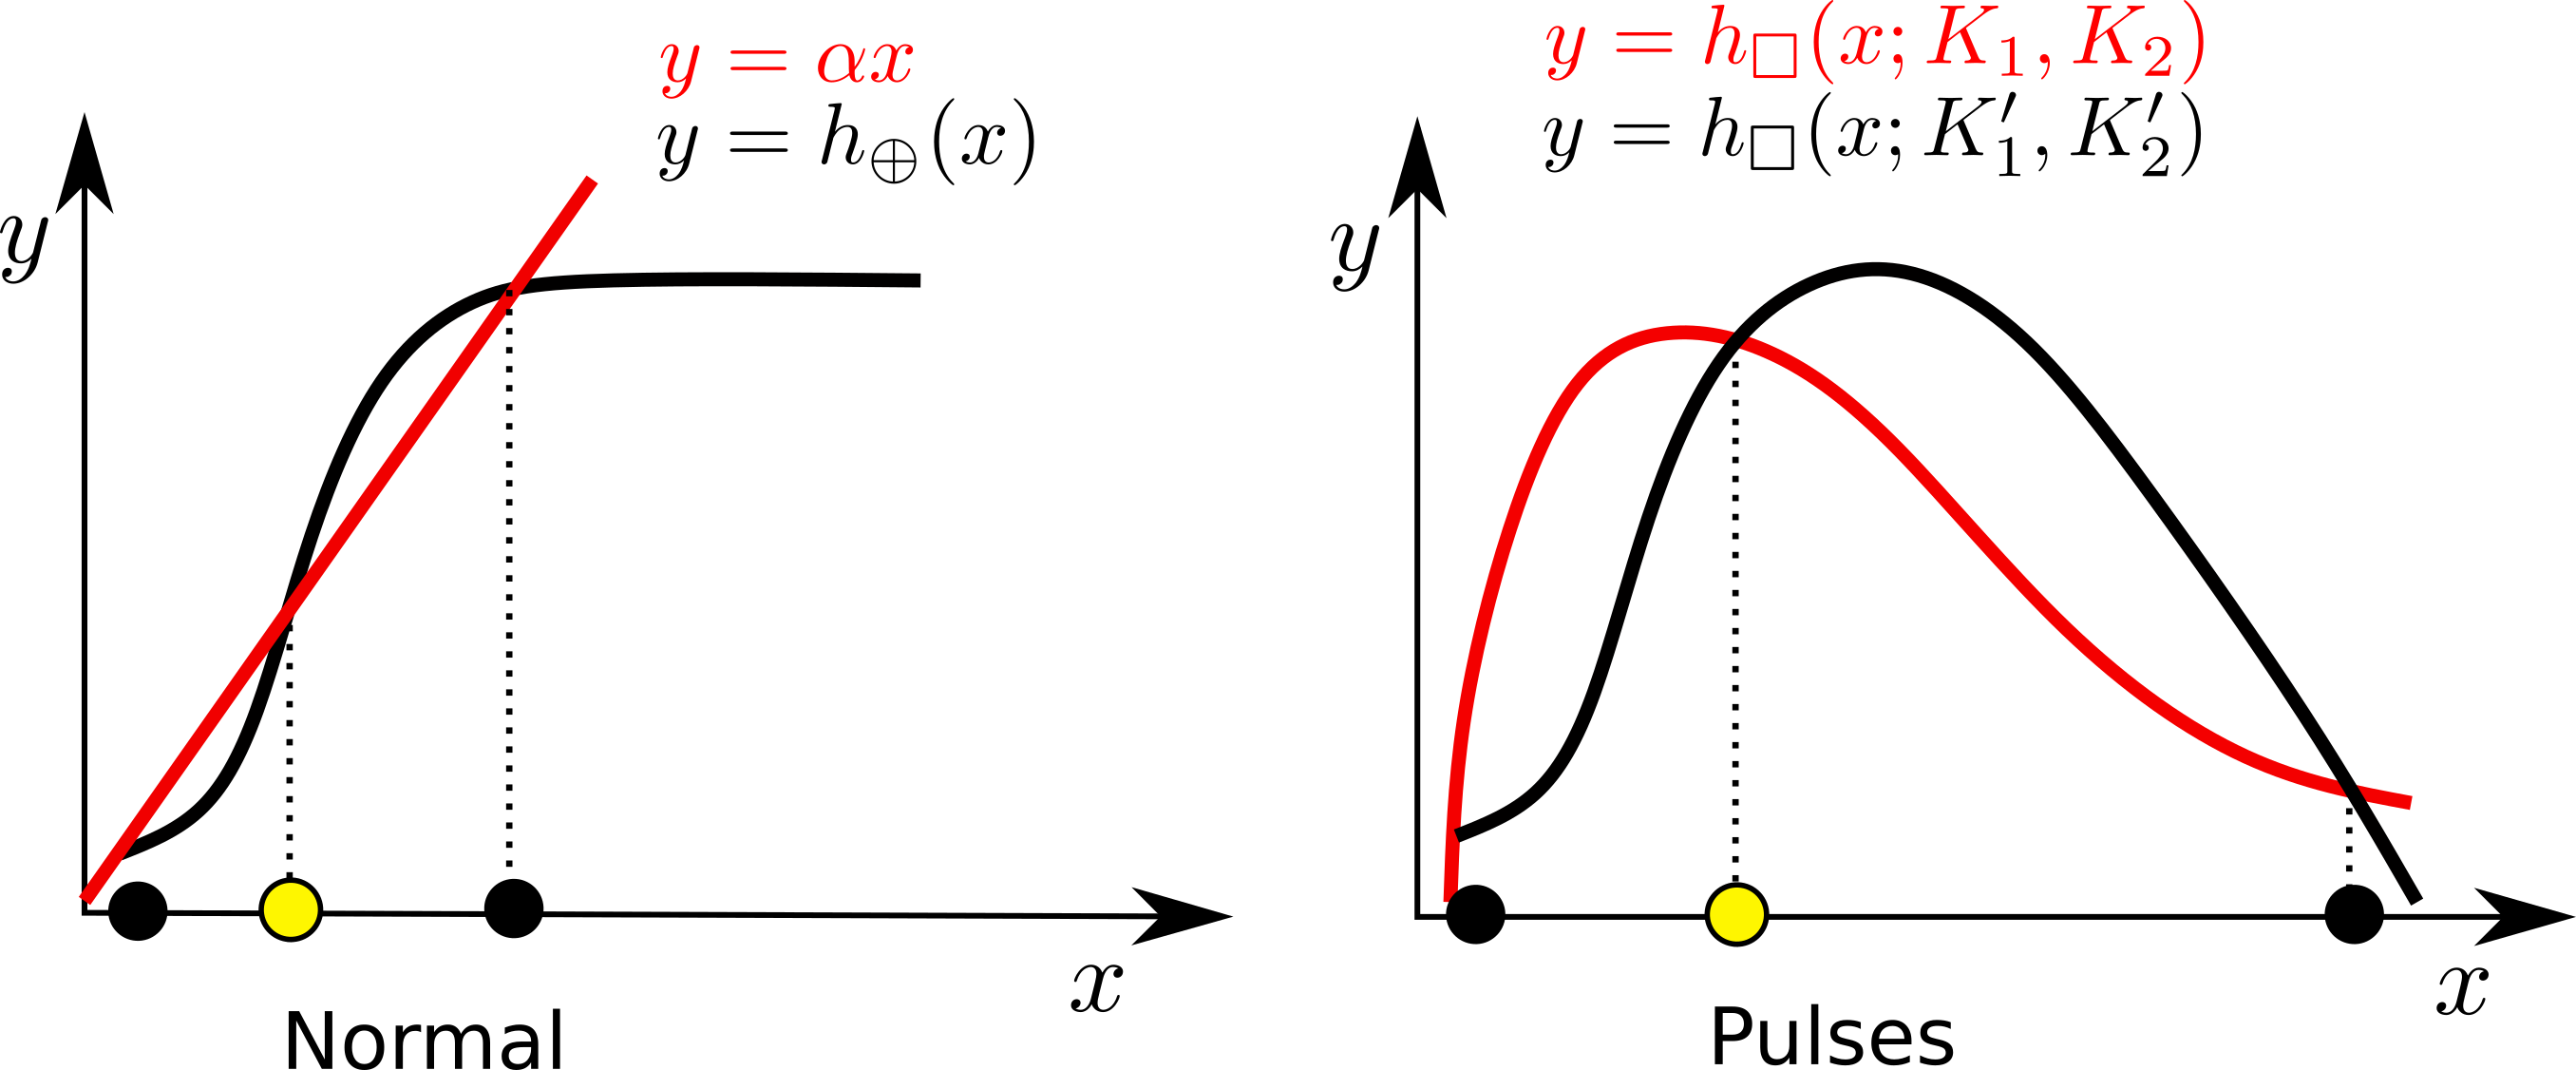
\includegraphics[width=4.7in]
{autoregulons/pulse-removal-production.png}
\caption{Removal and production under pulse.}
\label{fig-pulse-removal-production}
\end{figure}

\section{Biological basis for autoregulon networks}

If you are new to genomics, and would like to delve more deeply into the biological
basis of autoregulon networks, you might find
Alon's book Ref.\cite{alon-book} and Appendix \ref{ch-genomics-vocab} helpful.

\begin{figure}[h!]
\centering
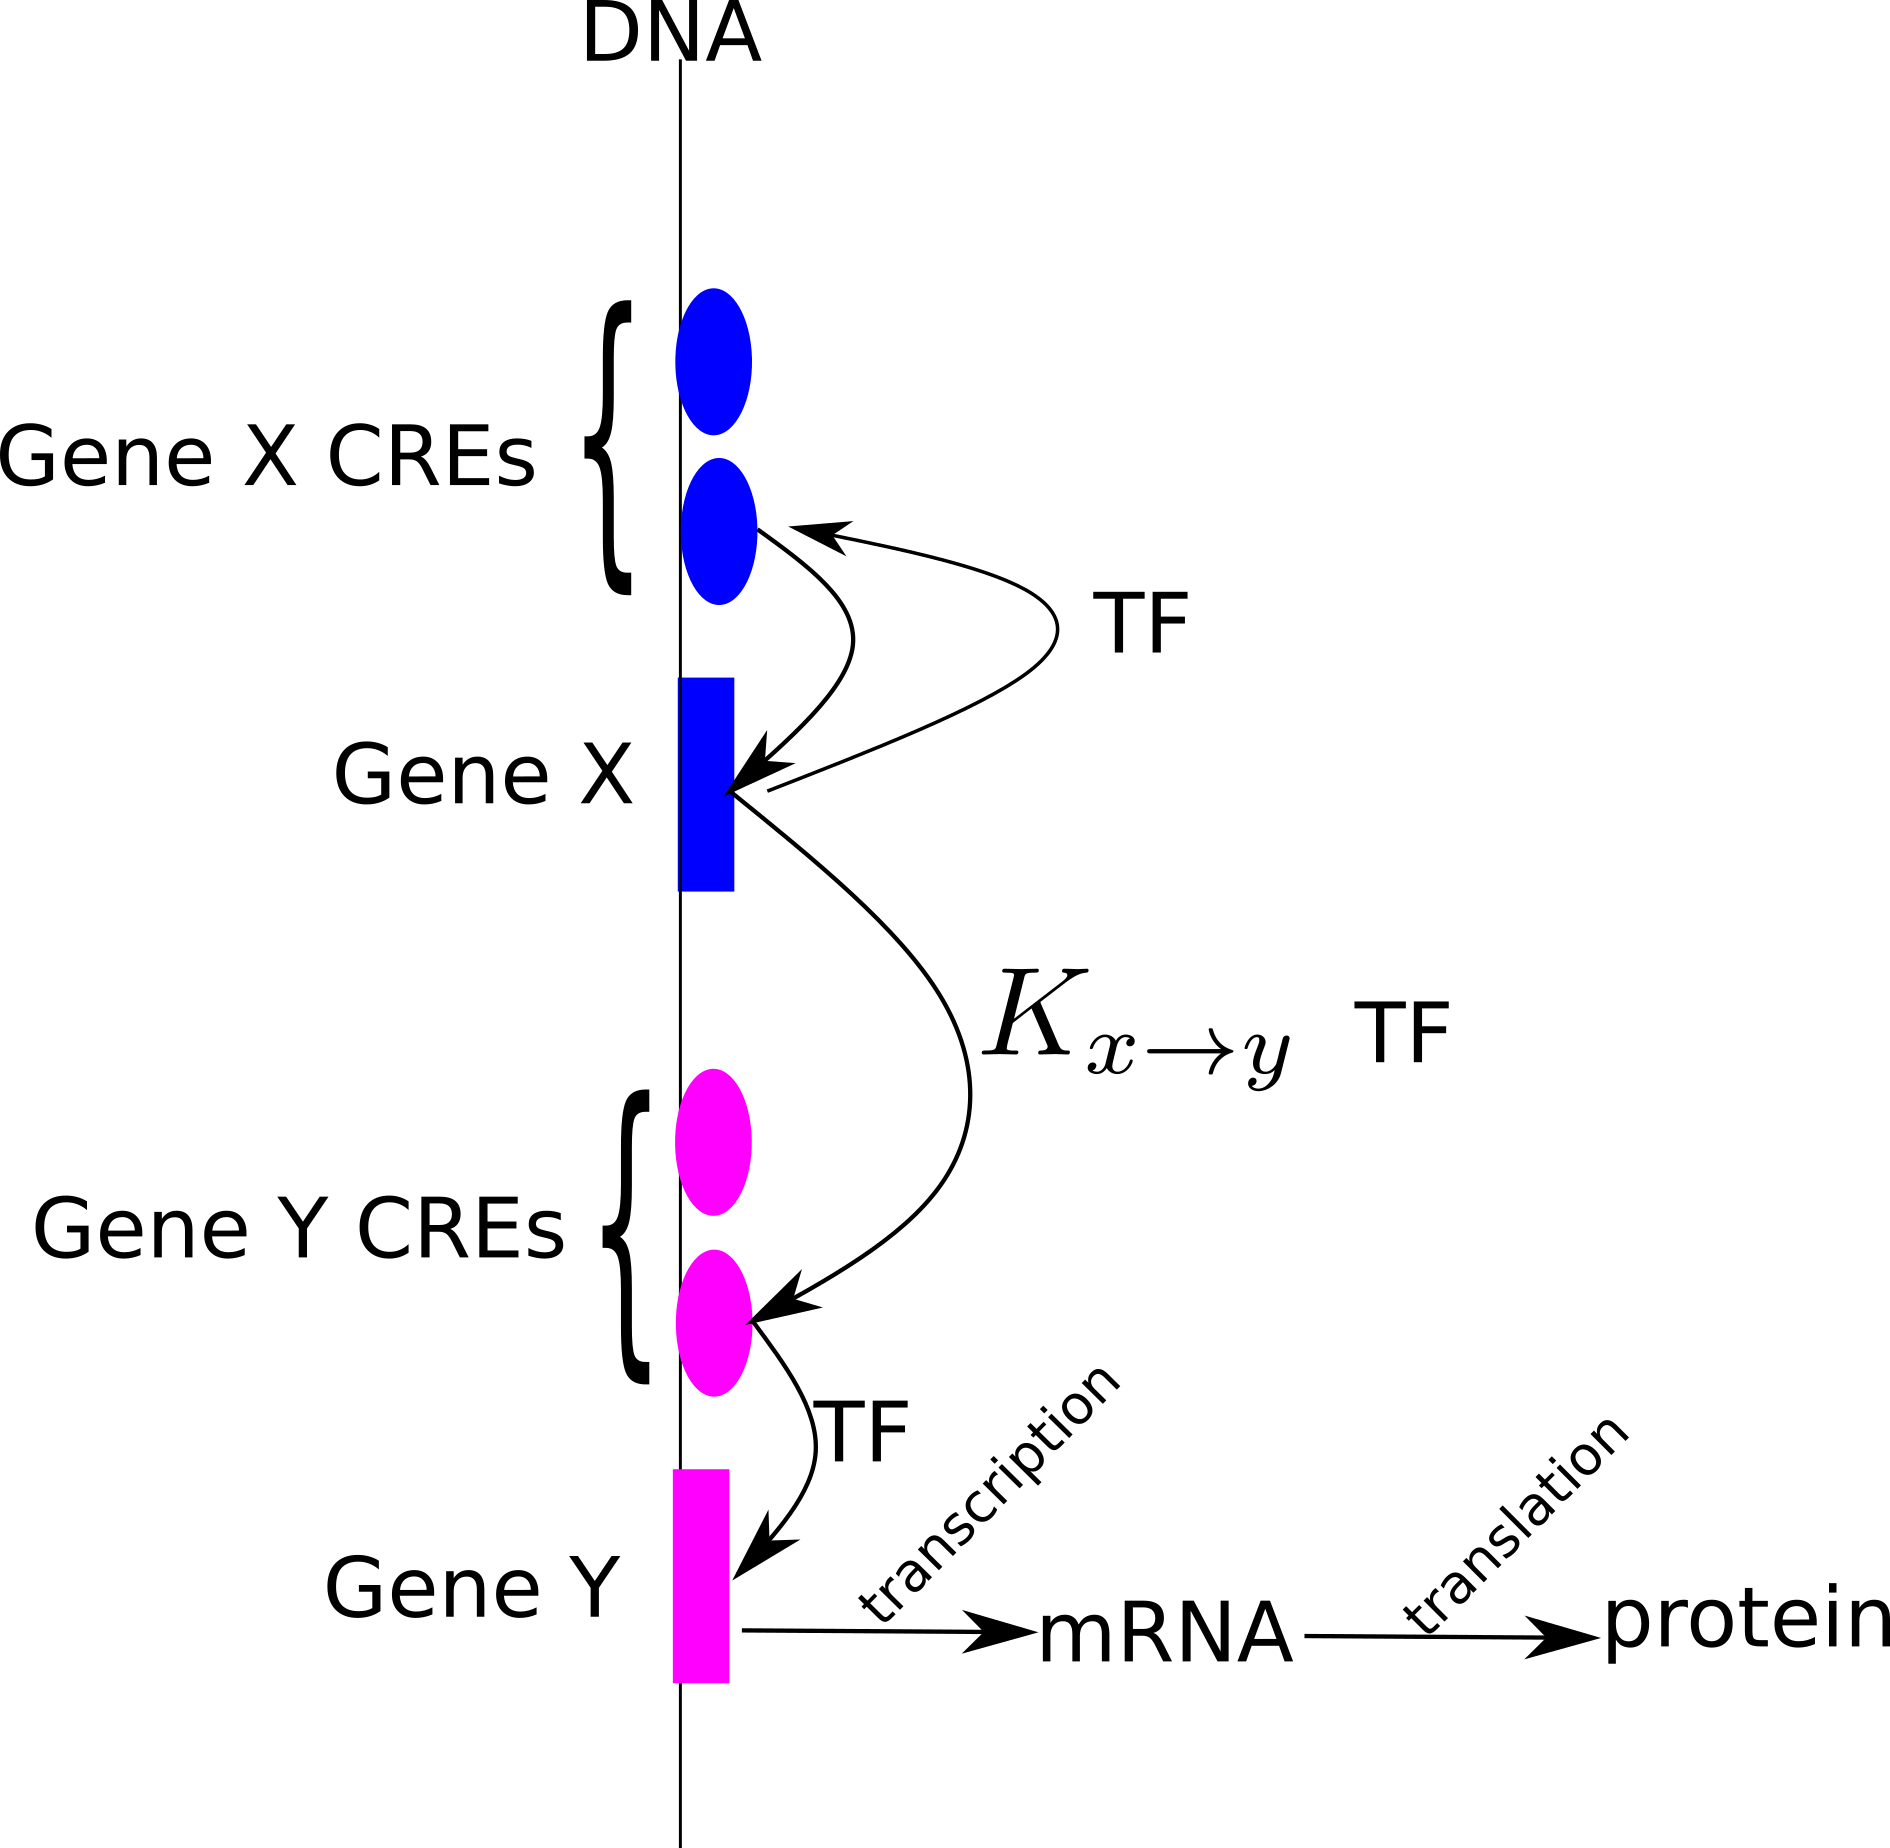
\includegraphics[width=2in]
{autoregulons/autoreg-bio.png}
\caption{Biological justification
for autoregulon math.  TF=transcription factor}
\label{fig-autoreg-bio}
\end{figure}

\section{Summary of Network Motifs}
Below, I include a very nice page from Ref.\cite{alon-book}.
I was going to re-write it in my own words, but
decided not to, so that the reader can get exposed to
the diagrammatic  notation, different from mine, used by experts in this field.
For this chapter, I've invented a diagrammatic
notation of my own that is more bnet like.

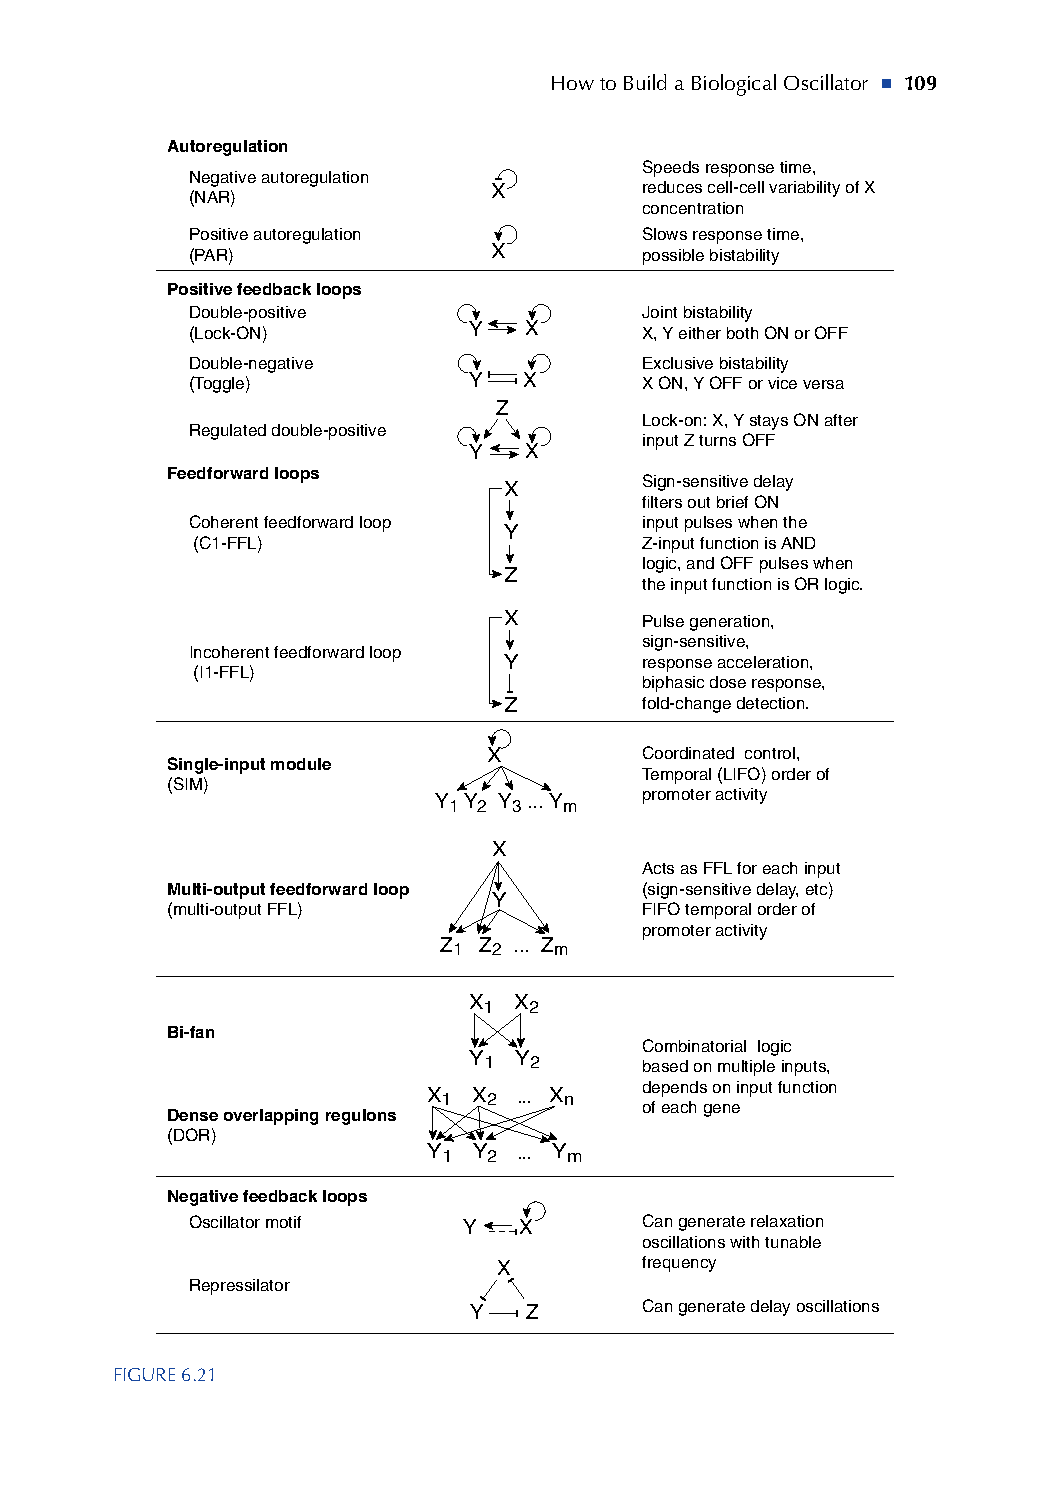
\includepdf[pages={1}]{autoregulons/alon-book-page-109.pdf}